%%%%%%%%%%%%%%%%%%%%%%%%%%%%%%%%%%%%%%%%%%%%%%%%%%%%%%%%%%%%%%%%%%%%%%%%%%%%%%%%%%%
%% Curtin Presentation Beamer Template                                           %%
%% Adapted from UFC template by
%% author: Maurício Moreira Neto - Doctoral student in Computer Science (MDCC)   %%
%%%%%%%%%%%%%%%%%%%%%%%%%%%%%%%%%%%%%%%%%%%%%%%%%%%%%%%%%%%%%%%%%%%%%%%%%%%%%%%%%%%

\documentclass{lib/curtin_format}
\usepackage{subcaption}
% Inserting the preamble file with the packages
%%%%%%%%%%%%%%%%%%%%%%%%%%%%%%%%%%%%%%%%%%%%%%%%%%%%%%%%%%%%%%%%%%%%%
%% This file contains the packages that can be used in the beamer. %%
%%%%%%%%%%%%%%%%%%%%%%%%%%%%%%%%%%%%%%%%%%%%%%%%%%%%%%%%%%%%%%%%%%%%%
% Package to fonts family
\usepackage[T1]{fontenc}
% Package to accentuation
\usepackage[utf8]{inputenc}
% Package to Portuguese language
%\usepackage[brazil]{babel}

%just in case eps figures are available instead - automatically converted to PDF
\usepackage{epstopdf}

% Package to Figures
\usepackage{graphicx}
% Package to the colors
\usepackage{color}
% Package to the colors
\usepackage{xcolor}
% Packages to math symbols and expressions
\usepackage{amsfonts, amssymb, amsmath}
% Package to multiple lines and columns in table
\usepackage{multirow, array} 
% Package to create pseudo-code
% For more detail of this package: http://linorg.usp.br/CTAN/macros/latex/contrib/algorithm2e/doc/algorithm2e.pdf
\usepackage{algorithm2e}
% Package to insert code
\usepackage{listings} 
\usepackage{keyval}
% Package to justify text
\usepackage[document]{ragged2e}
% Package to manage the bibliography
% \usepackage[backend=biber, style=numeric, sorting=none]{biblatex}
% Package to facilities quotations
\usepackage{csquotes}
% Package to use multicols
\usepackage{multicol}


% Inserting the references file
% \bibliography{references-crackseg.bib}
%\usepackage[style=author,backend=bibtex]{biblatex}
%\addbibresource{references.bib}

% \begin{figure}
%         \centering        
%         \includegraphics[width=2.00cm,height=1.00cm]{figs/ICONIP2021_logo.eps}
%         %\caption{Example of semantic segmentation}        
%         \label{fig:logo}
% 	\end{figure}	
% \vspace{-0.4cm}

% Title
\title[SC-CrackSeg]{\huge\textbf{SC-CrackSeg: A Real-time Shared Feature Pyramid
Network for Crack Detection and Segmentation}}
% Subtitle
%\subtitle{ICONIP 2021}

% Author of the presentation
\author{Moritz Bergemann \\ Supervised by Aneesh Krishna and Sonny Pham}
% Institute's Name
\institute[Curtin]{
    % email for contact
    \normalsize{\email{}}
    \newline
    % Department Name
    \department{School of EECMS}
    %\newline
    % university name
    \curtin
}
% date of the presentation
\date{}


%%%%%%%%%%%%%%%%%%%%%%%%%%%%%%%%%%%%%%%%%%%%%%%%%%%%%%%%%%%%%%%%%%%%%%%%%%%%%%%%%%
%% Start Document of the Presentation                                           %%               
%%%%%%%%%%%%%%%%%%%%%%%%%%%%%%%%%%%%%%%%%%%%%%%%%%%%%%%%%%%%%%%%%%%%%%%%%%%%%%%%%%
\begin{document}
% insert the code style
%%%%%%%%%%%%%%%%%%%%%%%%%%%%%%%%%%%%%%%%%%%%%%%%%%%%%%%%%%%%%%%%%%%%%%%%%%%%%%%%%%%
%% This file contains the style of the codes show in slides.                     %%
%% The package used is listings, but it possible to used others.                 %%
%%%%%%%%%%%%%%%%%%%%%%%%%%%%%%%%%%%%%%%%%%%%%%%%%%%%%%%%%%%%%%%%%%%%%%%%%%%%%%%%%%%

% color used in the code style
\definecolor{codegreen}{rgb}{0,0.6,0}
\definecolor{codegray}{rgb}{0.5,0.5,0.5}
\definecolor{codepurple}{rgb}{0.58,0,0.82}
\definecolor{codebackground}{rgb}{0.95,0.95,0.92}

% style of the code!
\lstdefinestyle{codestyle}{
    backgroundcolor=\color{codebackground},   
    commentstyle=\color{codegreen},
    keywordstyle=\color{magenta},
    numberstyle=\tiny\color{codegray},
    stringstyle=\color{codepurple},
    basicstyle=\ttfamily\footnotesize,
    frame=single,
    breakatwhitespace=false,         
    breaklines=true,                 
    captionpos=b,                    
    keepspaces=true,                 
    numbers=left,                    
    numbersep=5pt,                  
    showspaces=false,                
    showstringspaces=false,
    showtabs=false,                  
    tabsize=2,
    title=\lstname 
}

\lstset{style=codestyle}


%% ---------------------------------------------------------------------------
% First frame (with tile, subtitle, ...)
\begin{frame}{}

    \maketitle
    \vspace{-0.4cm}
    \begin{figure}
        \centering
        %\caption{Example of semantic segmentation}        
        \label{fig:logo}
    \end{figure}

\end{frame}

%% ---------------------------------------------------------------------------
% Second frame
\begin{frame}{Table of Contents}
    %\begin{multicols}{2}
    \tableofcontents
    %\end{multicols}
\end{frame}

%% ---------------------------------------------------------------------------
% This presentation is separated by sections and subsections
\section{Overview of key contributions}
\begin{frame}{Overview of key contributions}
    Our key contributions are:
    \begin{itemize}
        \item Introduce a new state-of-the-art model specifically designed for crack segmentation application task
        \item Assessed the unexplored field of domain adversarial semantic segmentation using transfomer models
        \item Evaluated lightweight segmentation transformers for unsupervised domain adaptation, and introduced novel pseudo-teacher approach for state-of-the-art results
    \end{itemize}
\end{frame}


\section{Crack Segmentation}
\begin{frame}{Crack Segmentation}
    \vspace{0.1cm}
    \begin{figure}
        \centering
        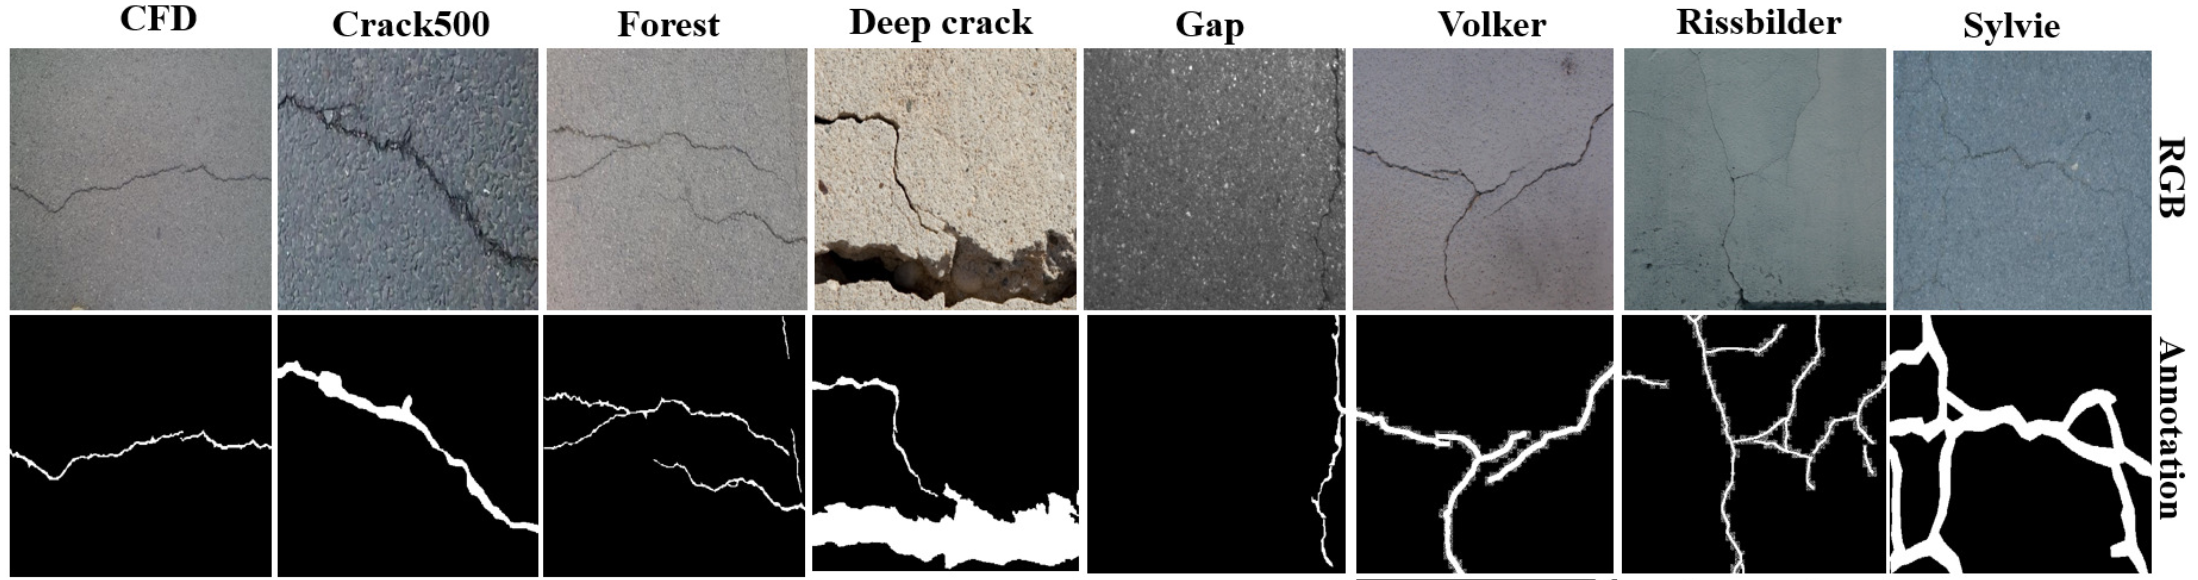
\includegraphics[width=1.05\linewidth]{res/crack-dataset.png}
        \caption{Crack dataset samples}
        \label{fig:crack-dataset}
    \end{figure}
\end{frame}

\begin{frame}{Our Architecture}
    \vspace{0.1cm}
    \begin{figure}
        \centering
        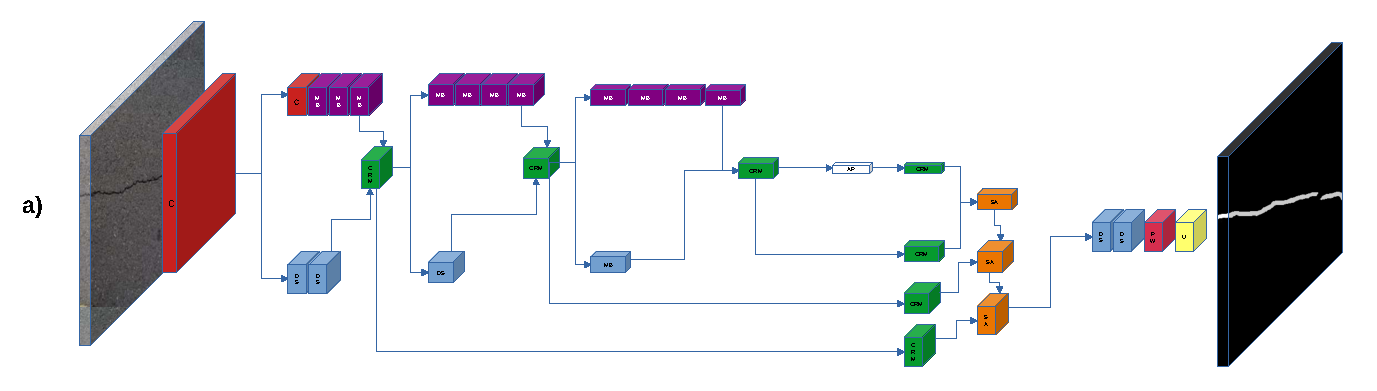
\includegraphics[width=\textwidth]{res/sc-crackseg.pdf}
        \caption{SC-CrackSeg}
        \label{fig:sc-crackseg-versions-sc-crackseg}
    \end{figure}
\end{frame}

\begin{frame}{SDDNet}
    \vspace{0.1cm}
    \begin{figure}
        \centering
        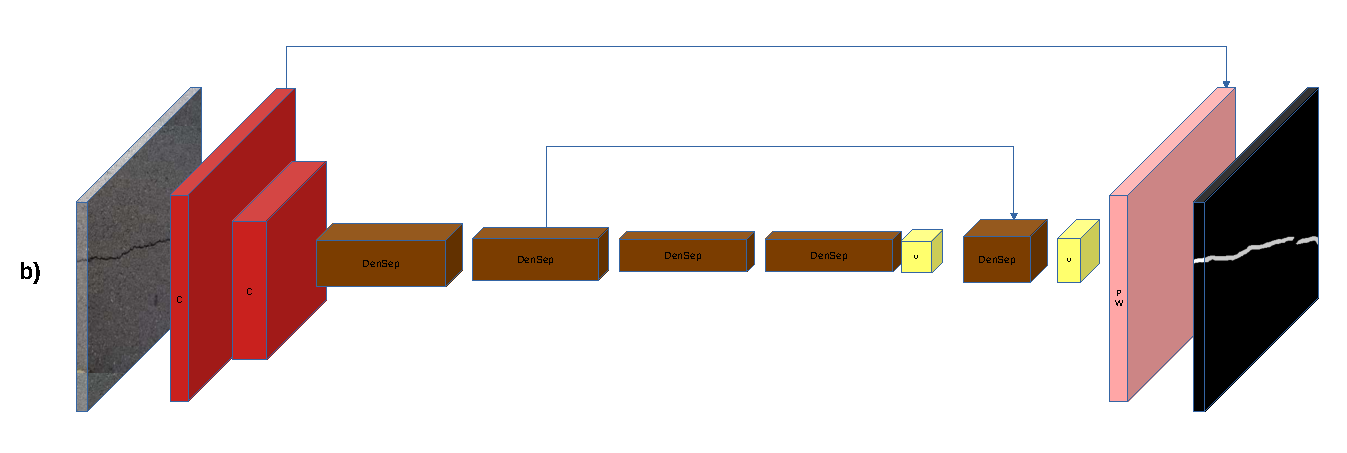
\includegraphics[width=\textwidth]{res/sddnet.pdf}
        \caption{SC-CrackSeg}
        \label{fig:sc-crackseg-versions-sddnet}
    \end{figure}
\end{frame}


\begin{frame}{SC-CrackSeg (Modified)}
    \vspace{0.1cm}
    \begin{figure}
        \centering
        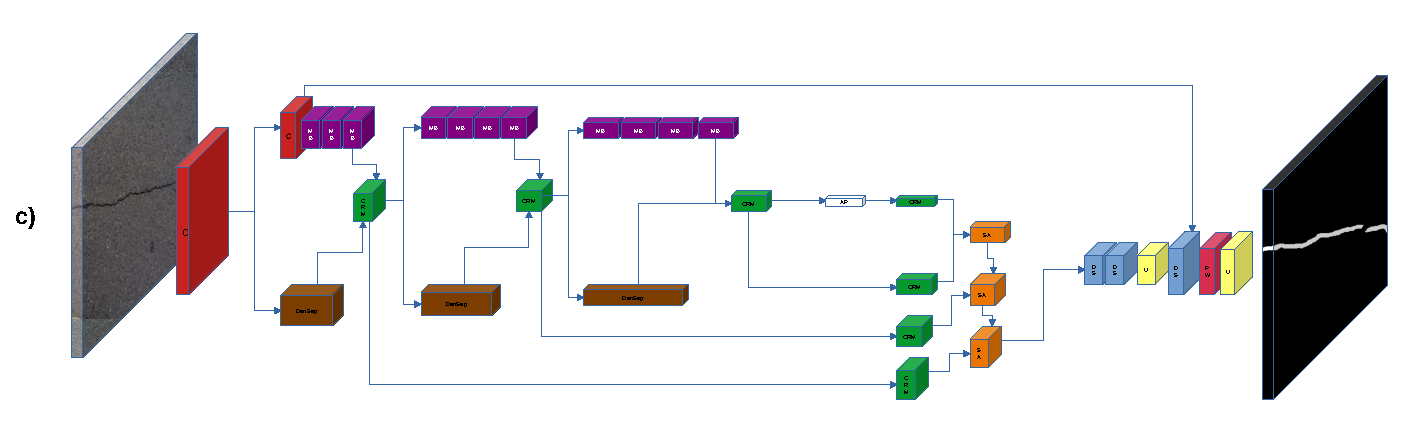
\includegraphics[width=\textwidth]{res/sc-crackseg-densep-skip.pdf}
        \caption{SC-CrackSeg}
        \label{fig:sc-crackseg-versions-sc-crackseg}
    \end{figure}
\end{frame}



\begin{frame}{Final Results}
    \begin{table}[]
        \resizebox{\textwidth}{!}{%
            \begin{tabular}{|p{0.2\textwidth}|c|c|c|c|c|c|c|c|}
                \hline
                                                              & \textbf{U-Net} & \textbf{SDDNet} & \textbf{SC-CrackSeg} & \textbf{SCMNet} & \textbf{SC-CrackSeg-1} & \textbf{SC-CrackSeg-2} & \textbf{SC-CrackSeg-3} & \textbf{SC-CrackSeg-4} \\
                \hline
                \textbf{Parameters}                           & 0.35M          & \textbf{0.33M}  & 1.27M                & 1.26M           & 0.63M                  & 1.01M                  & 1.51M                  & 1.3M                   \\
                \hline
                \textbf{FLOPs}                                & 2.44G          & 2.75G           & 1.4G                 & 1.62G           & 18.12G                 & \textbf{1.24G}         & 2.16G                  & 4.32G                  \\
                \hline
                \textbf{Crack Test Set Performance (\% mIoU)} & 0.796          & \textbf{0.815}  & 0.807                & 0.81            & 0.63                   & 0.808                  & 0.812                  & 0.803                  \\
                \hline
                \textbf{FPS}                                  & \textbf{27.05} & 15.84           & 15.94                & 16.87           & 12.75                  & 15.87                  & 14.01                  & 13.15                  \\
                \hline
            \end{tabular}
        }
        \caption{Performance evaluation of modifications (and SDDNet) on Crack Test set.}%\label{tab5}
        \label{}
    \end{table}
\end{frame}


\begin{frame}{Qualitative Results}
    \begin{figure}[htbp]
        \begin{tabular}{cccc}
            \begin{subfigure}[b]{0.23\textwidth}
                \centering
                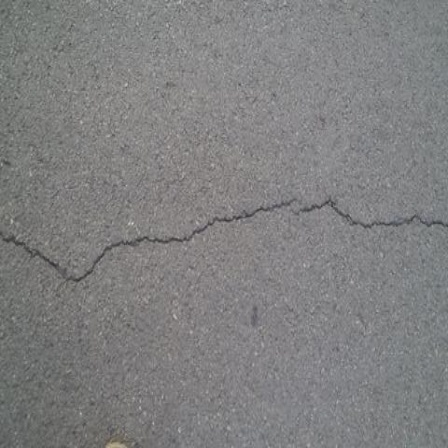
\includegraphics[width=\textwidth]{res/crackseg-experiment-qualitative/source.jpg}
                \caption{Source}
                \label{fig:crackseg-experiment-qualitative-source}
            \end{subfigure}
            \begin{subfigure}[b]{0.23\textwidth}
                \centering
                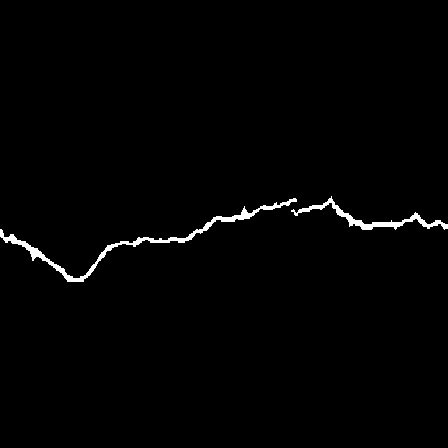
\includegraphics[width=\textwidth]{res/crackseg-experiment-qualitative/ground-truth.png}
                \caption{Ground Truth}
                \label{fig:crackseg-experiment-qualitative-ground-truth}
            \end{subfigure}
            \begin{subfigure}[b]{0.23\textwidth}
                \centering
                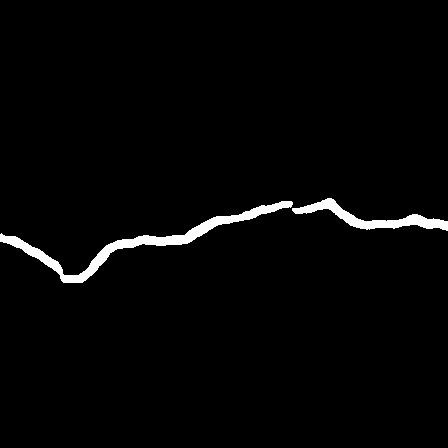
\includegraphics[width=\textwidth]{res/crackseg-experiment-qualitative/sddnet.png}
                \caption{SDDNet}
                \label{fig:crackseg-experiment-qualitative-sddnet}
            \end{subfigure}
            \begin{subfigure}[b]{0.23\textwidth}
                \centering
                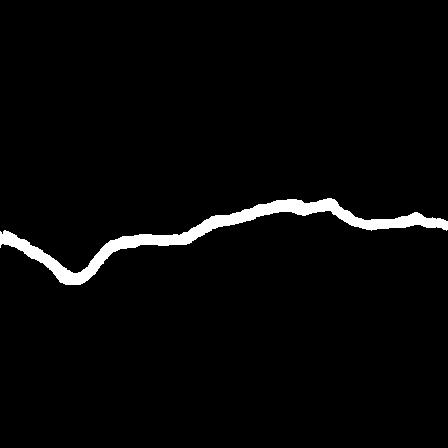
\includegraphics[width=\textwidth]{res/crackseg-experiment-qualitative/unet.png}
                \caption{U-Net}
                \label{fig:crackseg-experiment-qualitative-unet}
            \end{subfigure}
            \\
            \begin{subfigure}[b]{0.23\textwidth}
                \centering
                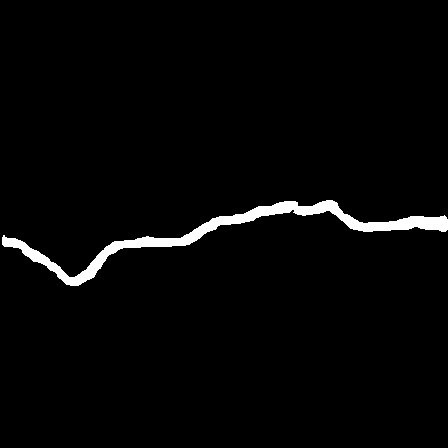
\includegraphics[width=\textwidth]{res/crackseg-experiment-qualitative/sc-crackseg.png}
                \caption{SC-CrackSeg}
                \label{fig:crackseg-experiment-qualitative-sc-crackseg}
            \end{subfigure}
            \begin{subfigure}[b]{0.23\textwidth}
                \centering
                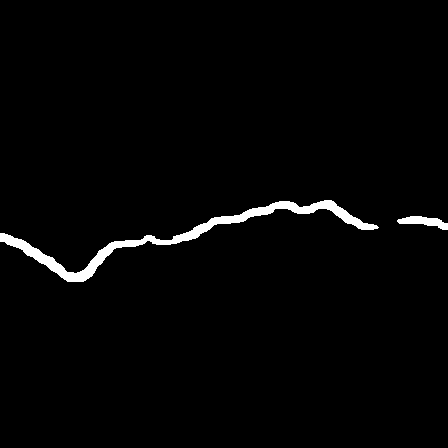
\includegraphics[width=\textwidth]{res/crackseg-experiment-qualitative/sc-crackseg-2.png}
                \caption{SC-CrackSeg-2}
                \label{fig:crackseg-experiment-qualitative-sc-crackseg-2}
            \end{subfigure}
            \begin{subfigure}[b]{0.23\textwidth}
                \centering
                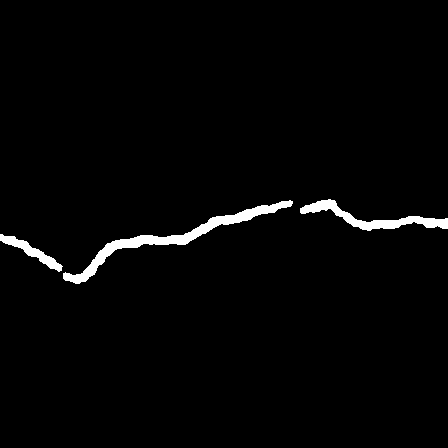
\includegraphics[width=\textwidth]{res/crackseg-experiment-qualitative/sc-crackseg-3.png}
                \caption{SC-CrackSeg-3}
                \label{fig:crackseg-experiment-qualitative-sc-crackseg-3}
            \end{subfigure}
            \begin{subfigure}[b]{0.23\textwidth}
                \centering
                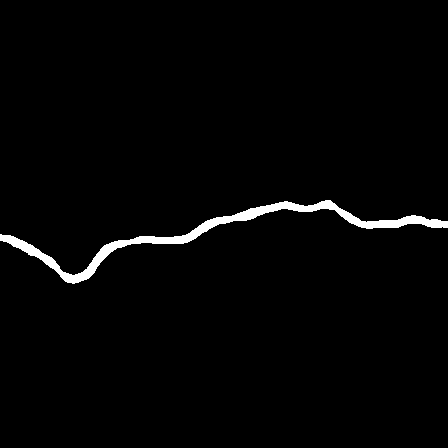
\includegraphics[width=\textwidth]{res/crackseg-experiment-qualitative/sc-crackseg-4.png}
                \caption{SC-CrackSeg-4}
                \label{fig:crackseg-experiment-qualitative-sc-crackseg-4}
            \end{subfigure}
        \end{tabular}
    \end{figure}
\end{frame}

\section{Domain Adversarial SegFormer}
\begin{frame}{Domain Adversarial Training}
    \begin{figure}[h]
        \centering
        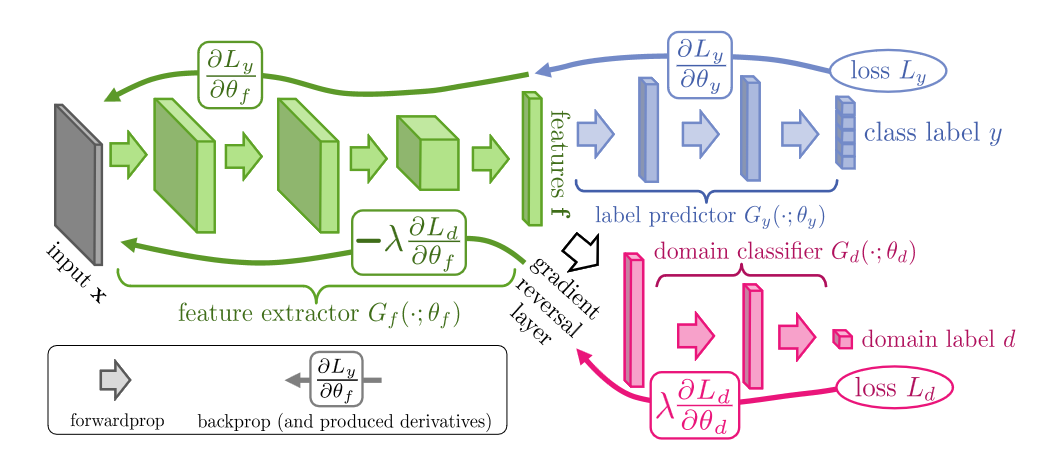
\includegraphics[width=\textwidth]{res/domain-adversarial-training.png}
        % \caption{Representation of domain adversarial training, retrieved from
        %     \cite{ganin_domain-adversarial_2016}}
        % \label{fig:domain-adversarial-training}
    \end{figure}
\end{frame}

\begin{frame}{Issue with Segmentation Transformers}
    \begin{table}[]
        \resizebox{\textwidth}{!}{%
            \begin{tabular}{|l|r|r|r|}
                \hline
                Model                 & mIoU (source-only) & mIoU (with discriminator) & Relative Change \\
                \hline
                DeelabV3+ (ResNet-50) & 33.9               & 35.97                     & +2.07           \\
                \hline
                SegFormer (MiT-B3)    & 41.78              & 39.38                     & -2.40           \\
                \hline
            \end{tabular}
        }
        % \caption{Baseline experiment results comparing SegFormer and DeeplabV3+. Both experiments used a simplified DCGAN-like \cite{radford_unsupervised_2016} discriminator consisting of 3 convolutional layers with 64, 128, and 2 channels respectively.}
        % \label{tab:das-baseline-experiment}
    \end{table}
\end{frame}


\begin{frame}{DAS Patchwise Architecture}
    \begin{figure}[]
        \centering
        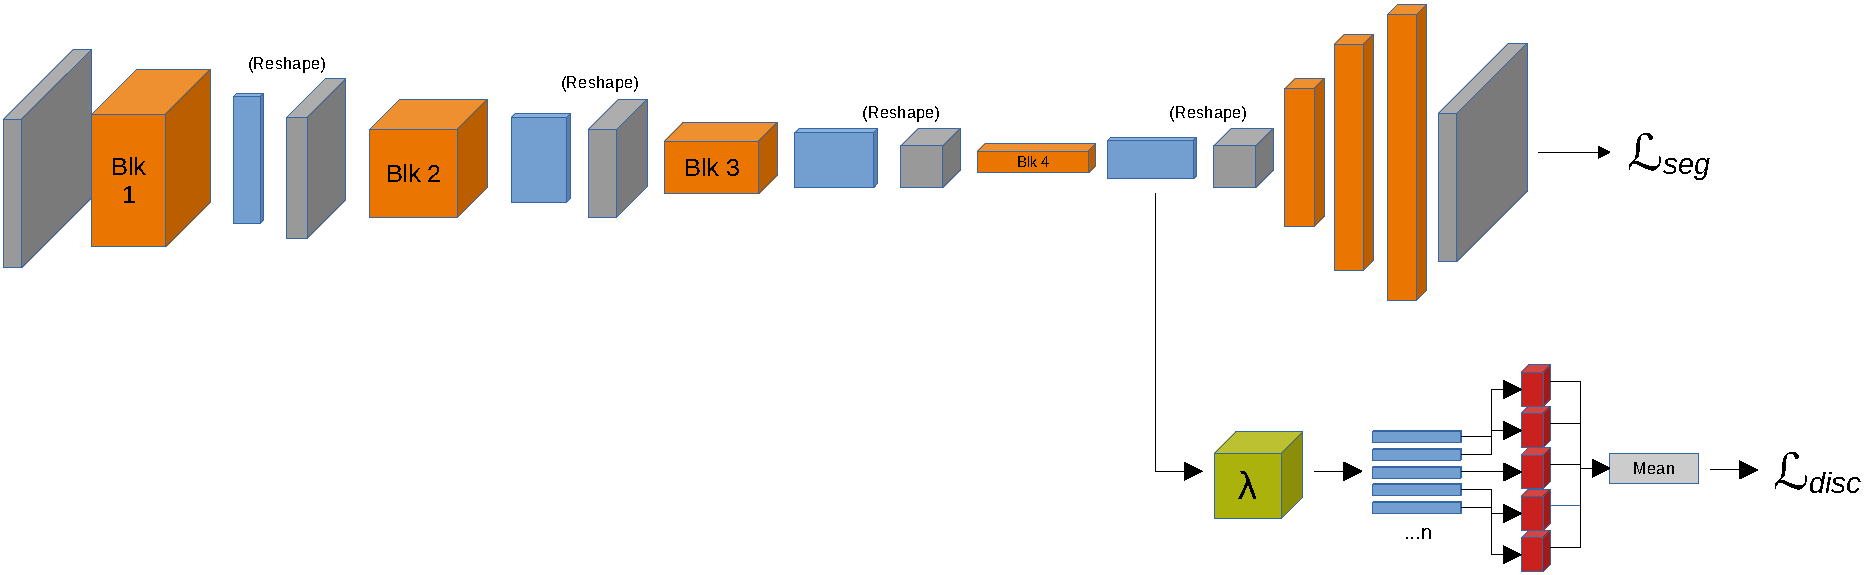
\includegraphics[width=\textwidth]{res/discriminator-diagrams/patch.pdf}
        \label{fig:das-discriminators-patch-wise}
    \end{figure}
\end{frame}

\begin{frame}{DAS DCGAN Architecture}
    \begin{figure}[]
        \centering
        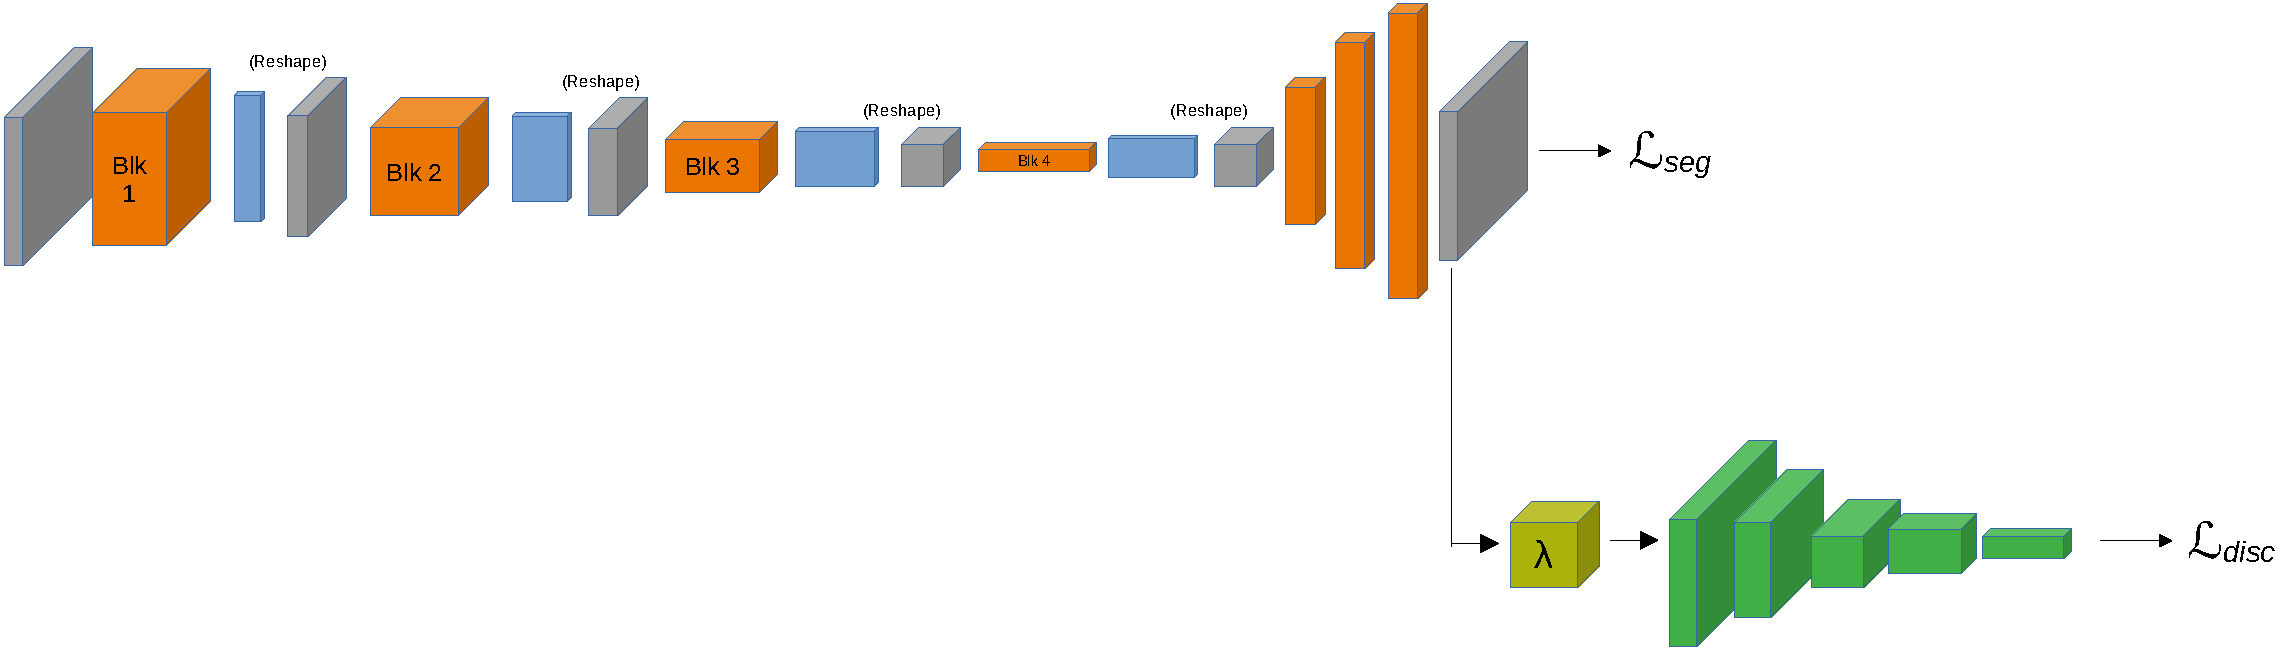
\includegraphics[width=\textwidth]{res/discriminator-diagrams/dcgan-output.pdf}
        \label{fig:das-discriminators-dcgan}
    \end{figure}
\end{frame}

\begin{frame}{Final Best Results}
    \begin{figure}[h]
        \centering
        \begin{tabular}{|l|l|r|}
            \hline
            Auxiliary Method            & Discriminator & \multicolumn{1}{l|}{mIoU} \\ \hline
            RCS                         & DCGAN         & \textbf{44.76}            \\ \hline
            Class distribution matching & DCGAN         & 39.4                      \\ \hline
            Fine class matching         & DCGAN         & 37.22                     \\ \hline
            Source-Only                 & -             & 41.78                     \\ \hline
        \end{tabular}
        % \caption{Results of auxiliary approaches on DAS. Adding RCS improves performance over baseline.}
    \end{figure}
\end{frame}

\begin{frame}{Final Best Results}
    \begin{figure}[]
        % \resizebox{\textwidth}{!}{%
        \centering
        \begin{tabular}{llll}
            Source Image                                                              & Ground Truth                                                               \\
            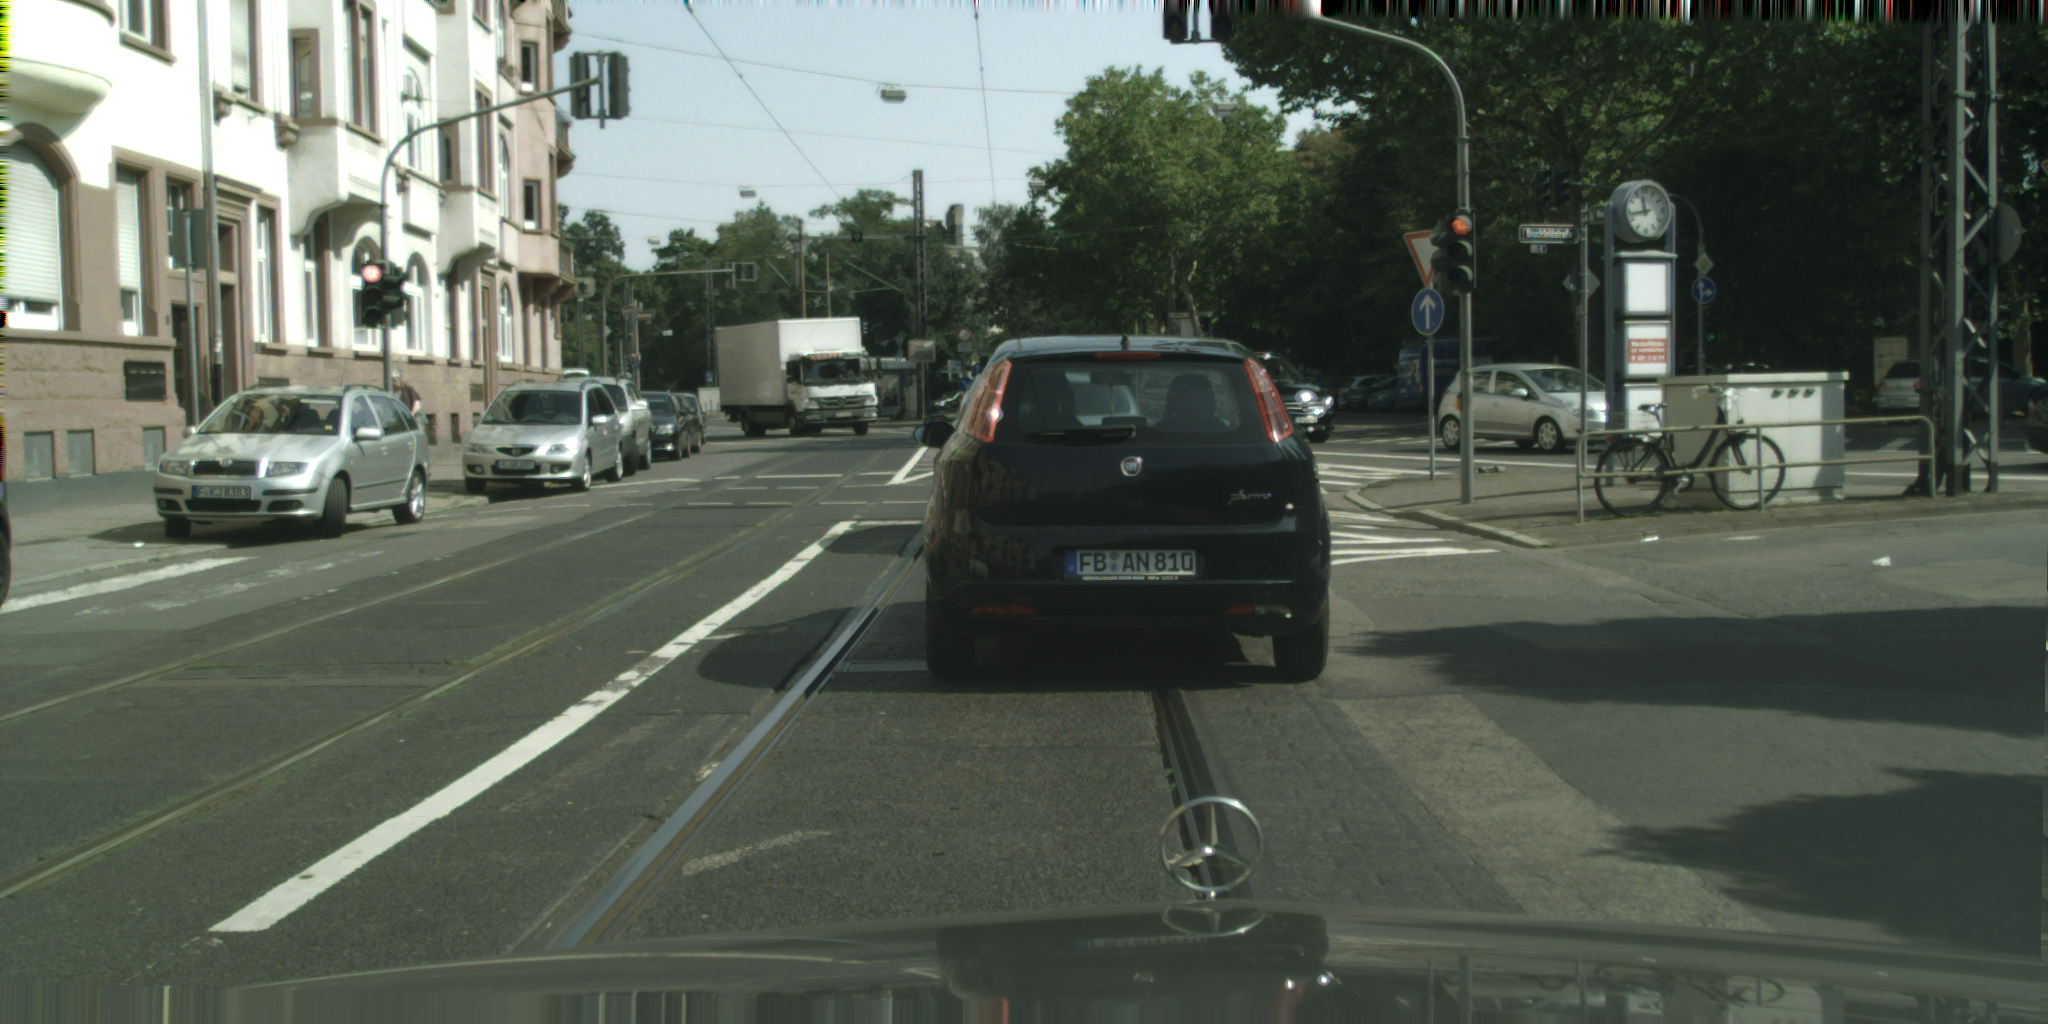
\includegraphics[width=.4\linewidth]{res/das-qualitative/image.png}       & 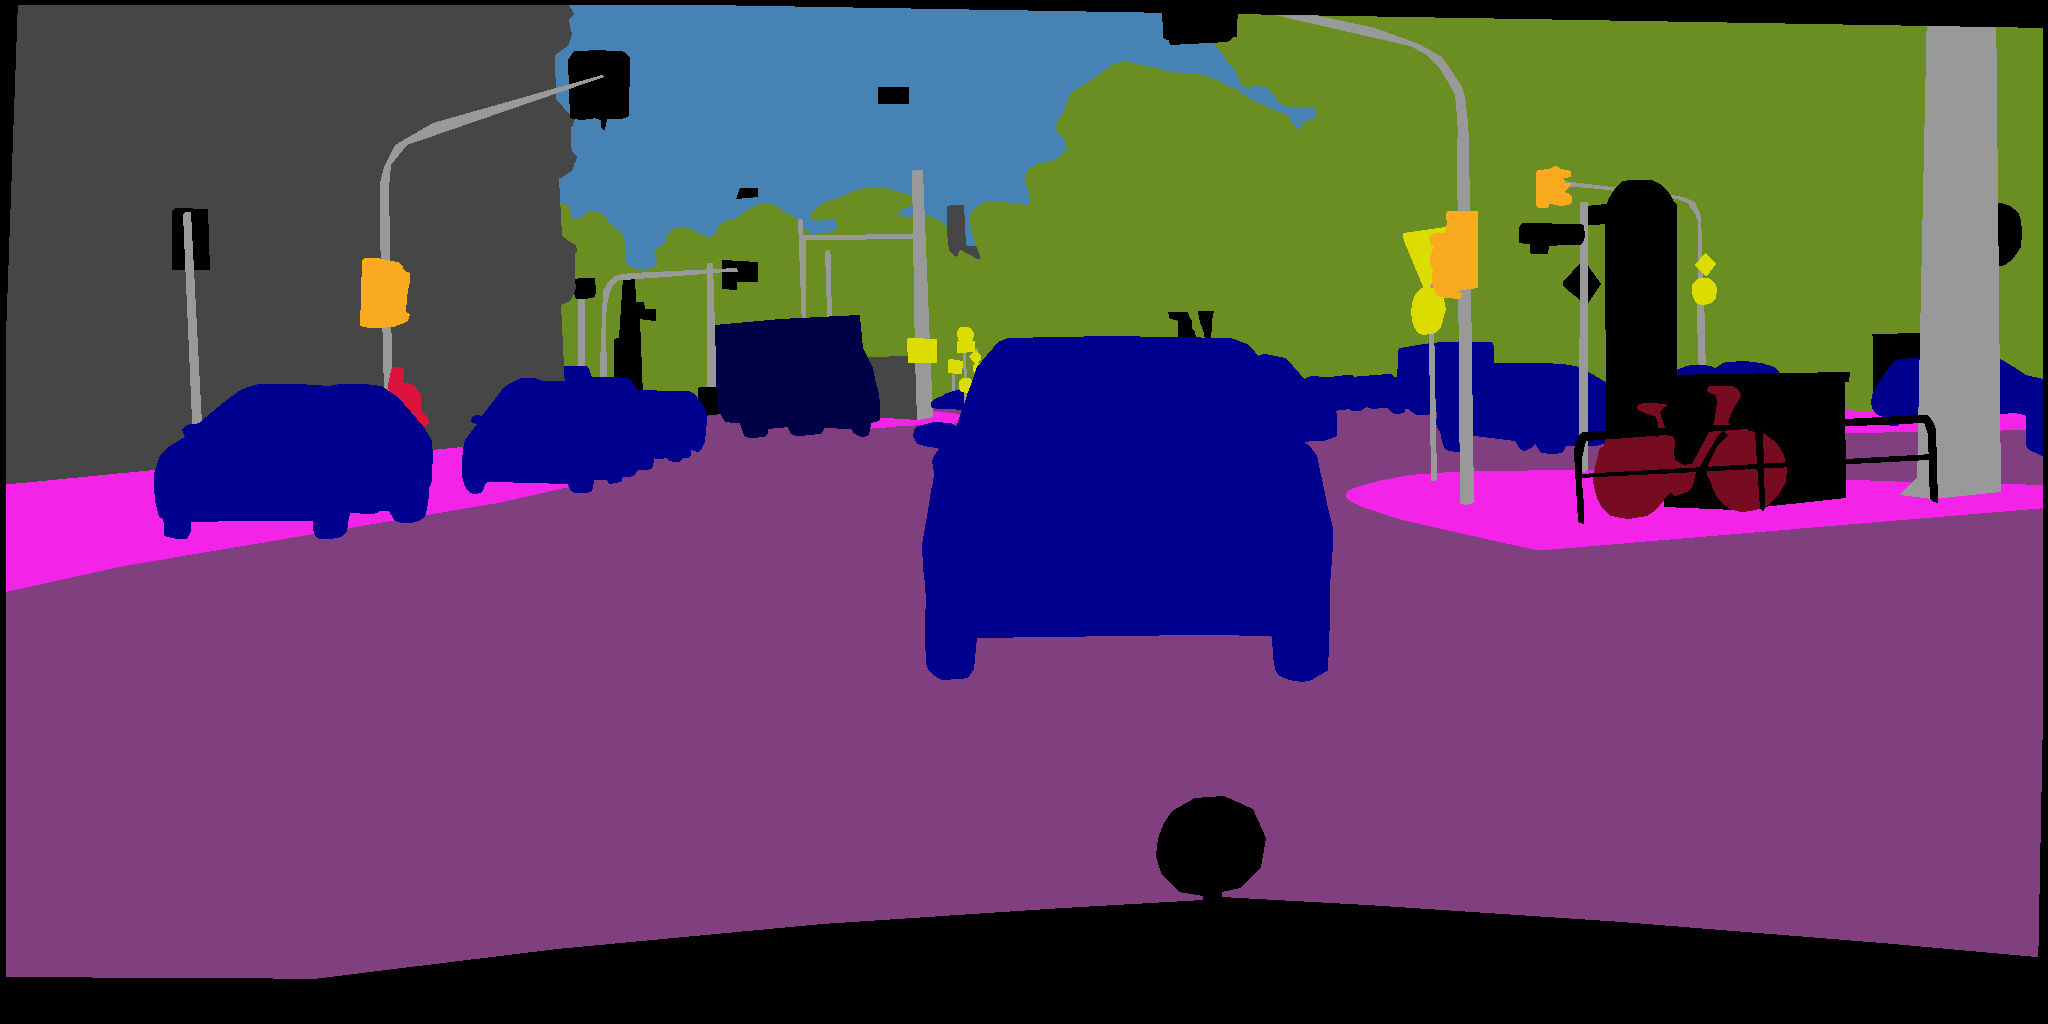
\includegraphics[width=.4\linewidth]{res/das-qualitative/ground-truth.png} \\
            Source-Only                                                               & DCGAN + RCS                                                                \\
            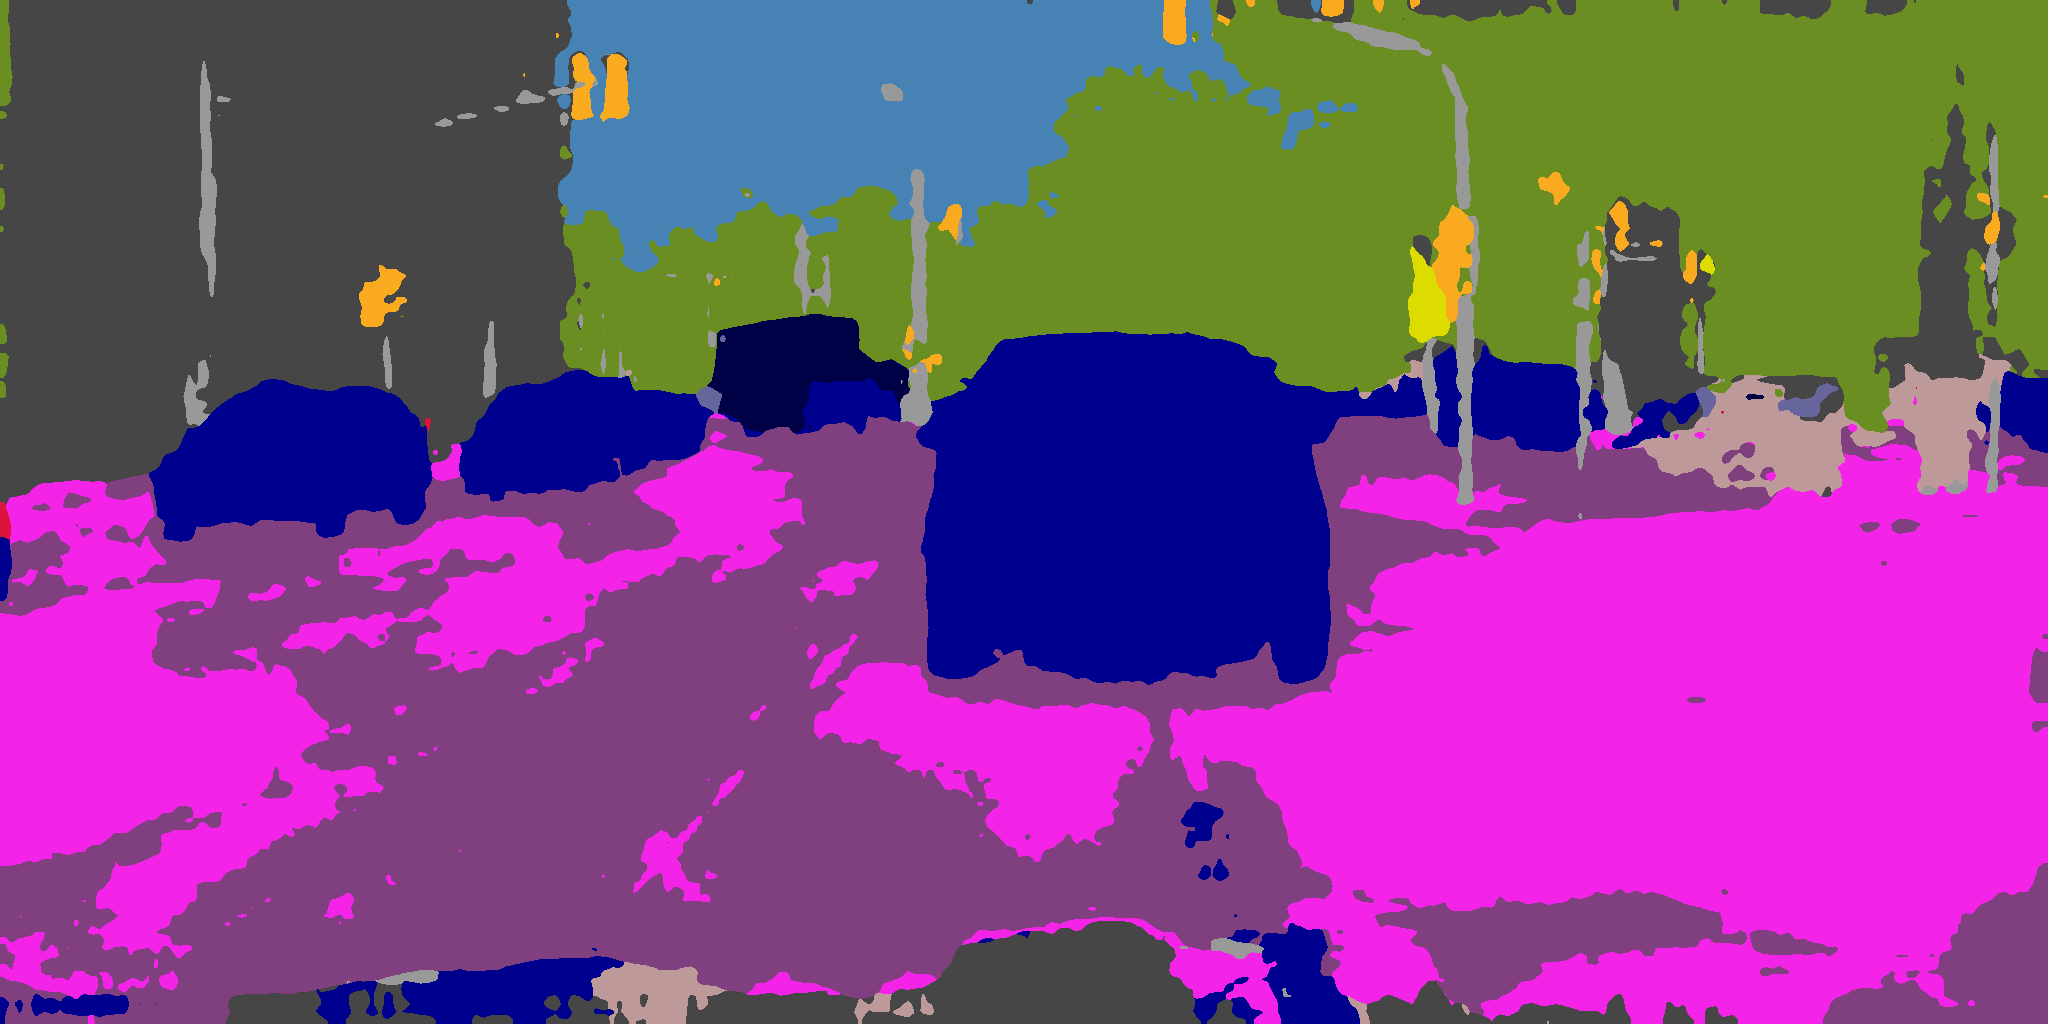
\includegraphics[width=.4\linewidth]{res/das-qualitative/source-only.png} & 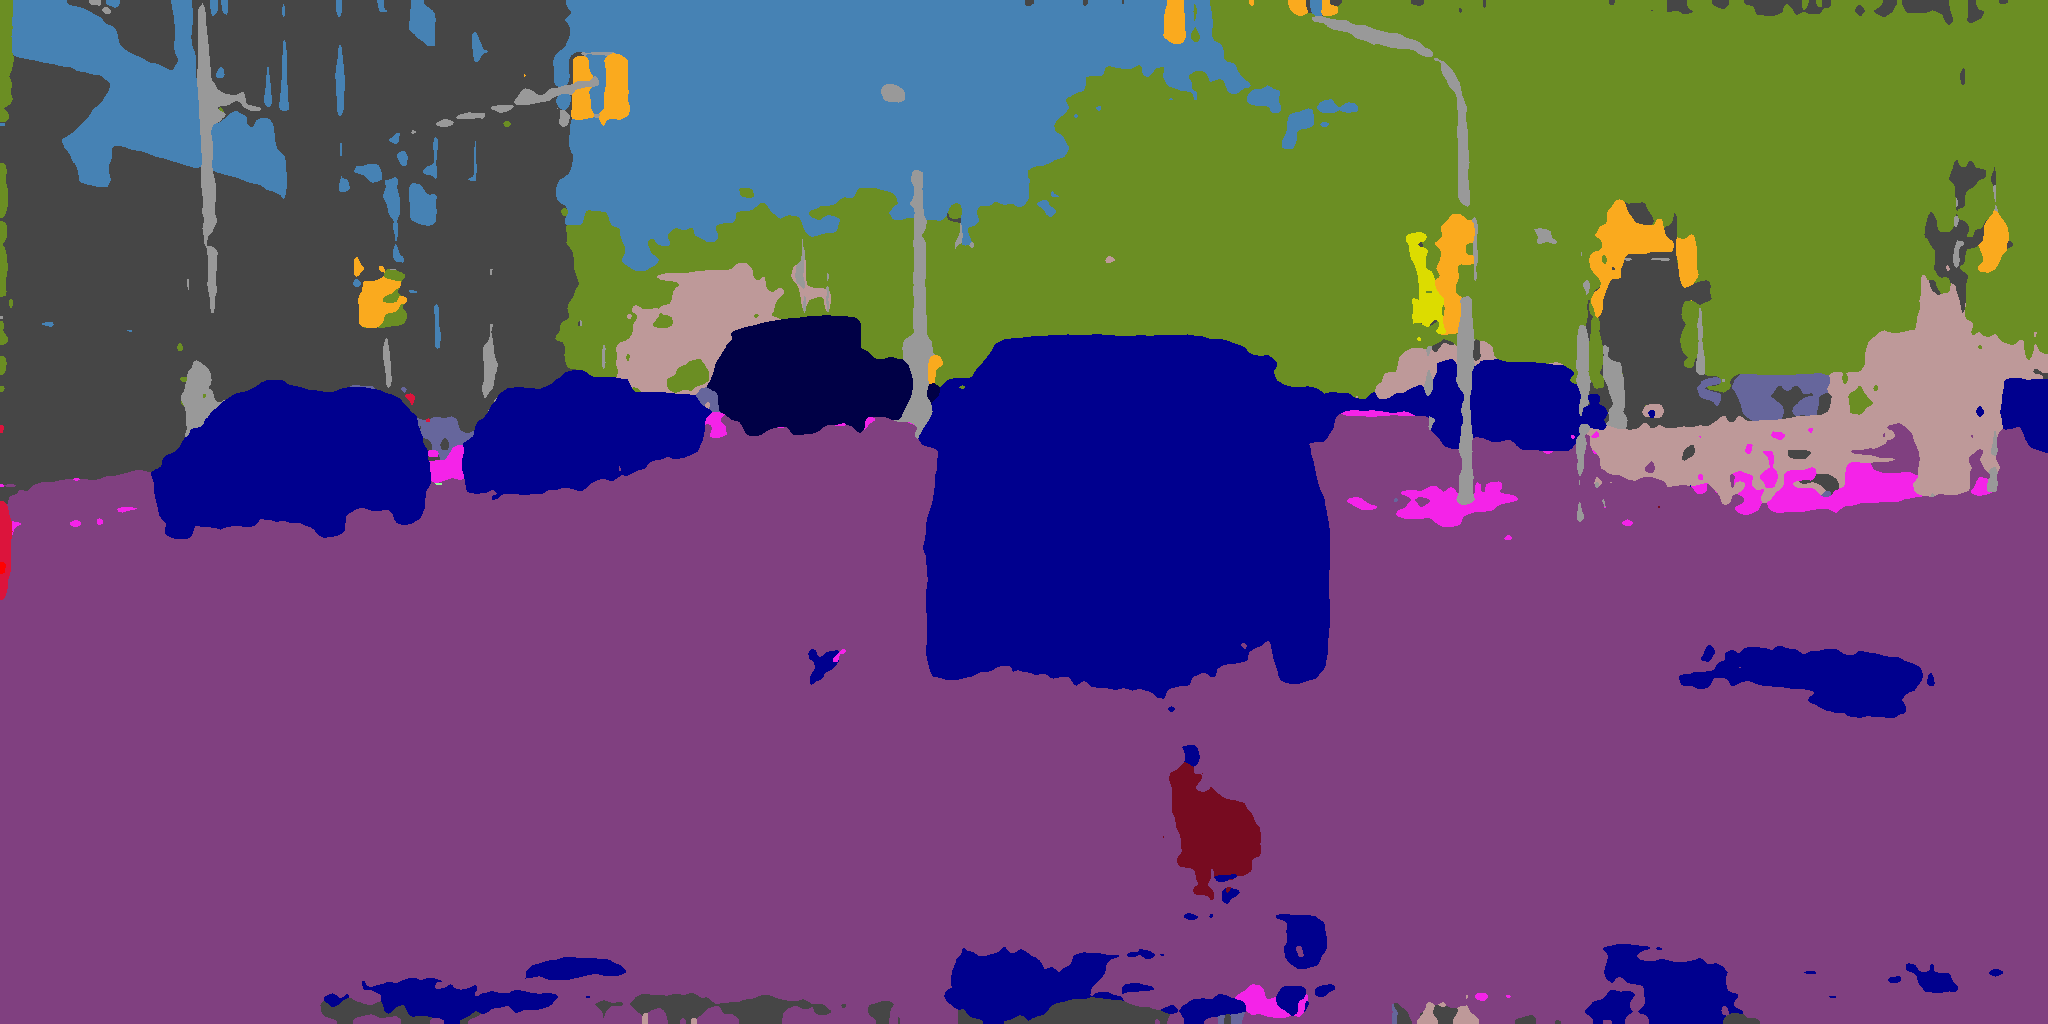
\includegraphics[width=.4\linewidth]{res/das-qualitative/dcgan-rcs.png}    \\
        \end{tabular}
        \caption{Comparison of DCGAN + RCS DAS against source-only training.}
        \label{fig:das-qualitative}
    \end{figure}
\end{frame}

\section{Pseudo-teacher training}

\begin{frame}{Baseline Comparison}

    \begin{table}[]
        \resizebox{\textwidth}{!}{%
            \begin{tabular}{|l|l|r|l|r|r|r|}
                \hline
                Model                & \begin{tabular}[c]{@{}l@{}}Reported\\ Params\end{tabular} & \multicolumn{1}{l|}{\begin{tabular}[c]{@{}l@{}}Measured \\ Params (M)\end{tabular}} & \begin{tabular}[c]{@{}l@{}}Reported \\ FLOPs \\ (GFlops)\end{tabular} & \multicolumn{1}{l|}{\begin{tabular}[c]{@{}l@{}}Measured \\ FLOPs \\ (GFlops)\end{tabular}} & \multicolumn{1}{l|}{\begin{tabular}[c]{@{}l@{}}mIoU \\ (Source-Only)\end{tabular}} & \multicolumn{1}{l|}{\begin{tabular}[c]{@{}l@{}}mIoU \\ (UDA)\end{tabular}} \\ \hline
                Fast-SCNN            & 1.11M                                                     & 1.46                                                                                & -                                                                     & \textbf{0.94}                                                                              & 20.95                                                                              & \multicolumn{1}{l|}{-}                                                     \\ \hline
                Segformer(MiT-B0)    & 3.8M                                                      & 6.09                                                                                & \multicolumn{1}{r|}{8.4}                                              & 42.94                                                                                      & 26.57                                                                              & 47.55                                                                      \\ \hline
                DAFormer (MiT-B0)    & -                                                         & 4.26                                                                                & -                                                                     & 17.69                                                                                      & 28.12                                                                              & \textbf{50.56}                                                             \\ \hline
                MobileViT (Small)    & 6.4 M                                                     & 12.65                                                                               & -                                                                     & 16.93                                                                                      & 31.86                                                                              & 46.73                                                                      \\ \hline
                MobileViT (XX-Small) & -                                                         & 6.28                                                                                & -                                                                     & 7.08                                                                                       & 30.35                                                                              & 41.38                                                                      \\ \hline
                TopFormer (Base)     & 5.1M                                                      & 1.81                                                                                & \multicolumn{1}{r|}{2.7}                                              & 5.06                                                                                       & \textbf{33.32}                                                                     & 43.15                                                                      \\ \hline
                TopFormer (Tiny)     & 1.4M                                                      & \textbf{1.39}                                                                       & -                                                                     & 0.58                                                                                       & 27.78                                                                              & 36.98                                                                      \\ \hline
            \end{tabular}
        }
        % \caption{Baseline experiment results comparing SegFormer and DeeplabV3+. Both experiments used a simplified DCGAN-like \cite{radford_unsupervised_2016} discriminator consisting of 3 convolutional layers with 64, 128, and 2 channels respectively.}
        % \label{tab:das-baseline-experiment}
    \end{table}
\end{frame}

\begin{frame}{Baseline Qualitative Comparison}
    \begin{figure}[]
        % \resizebox{\textwidth}{!}{%
        \centering
        \begin{tabular}{lll}
            Ground Truth   & 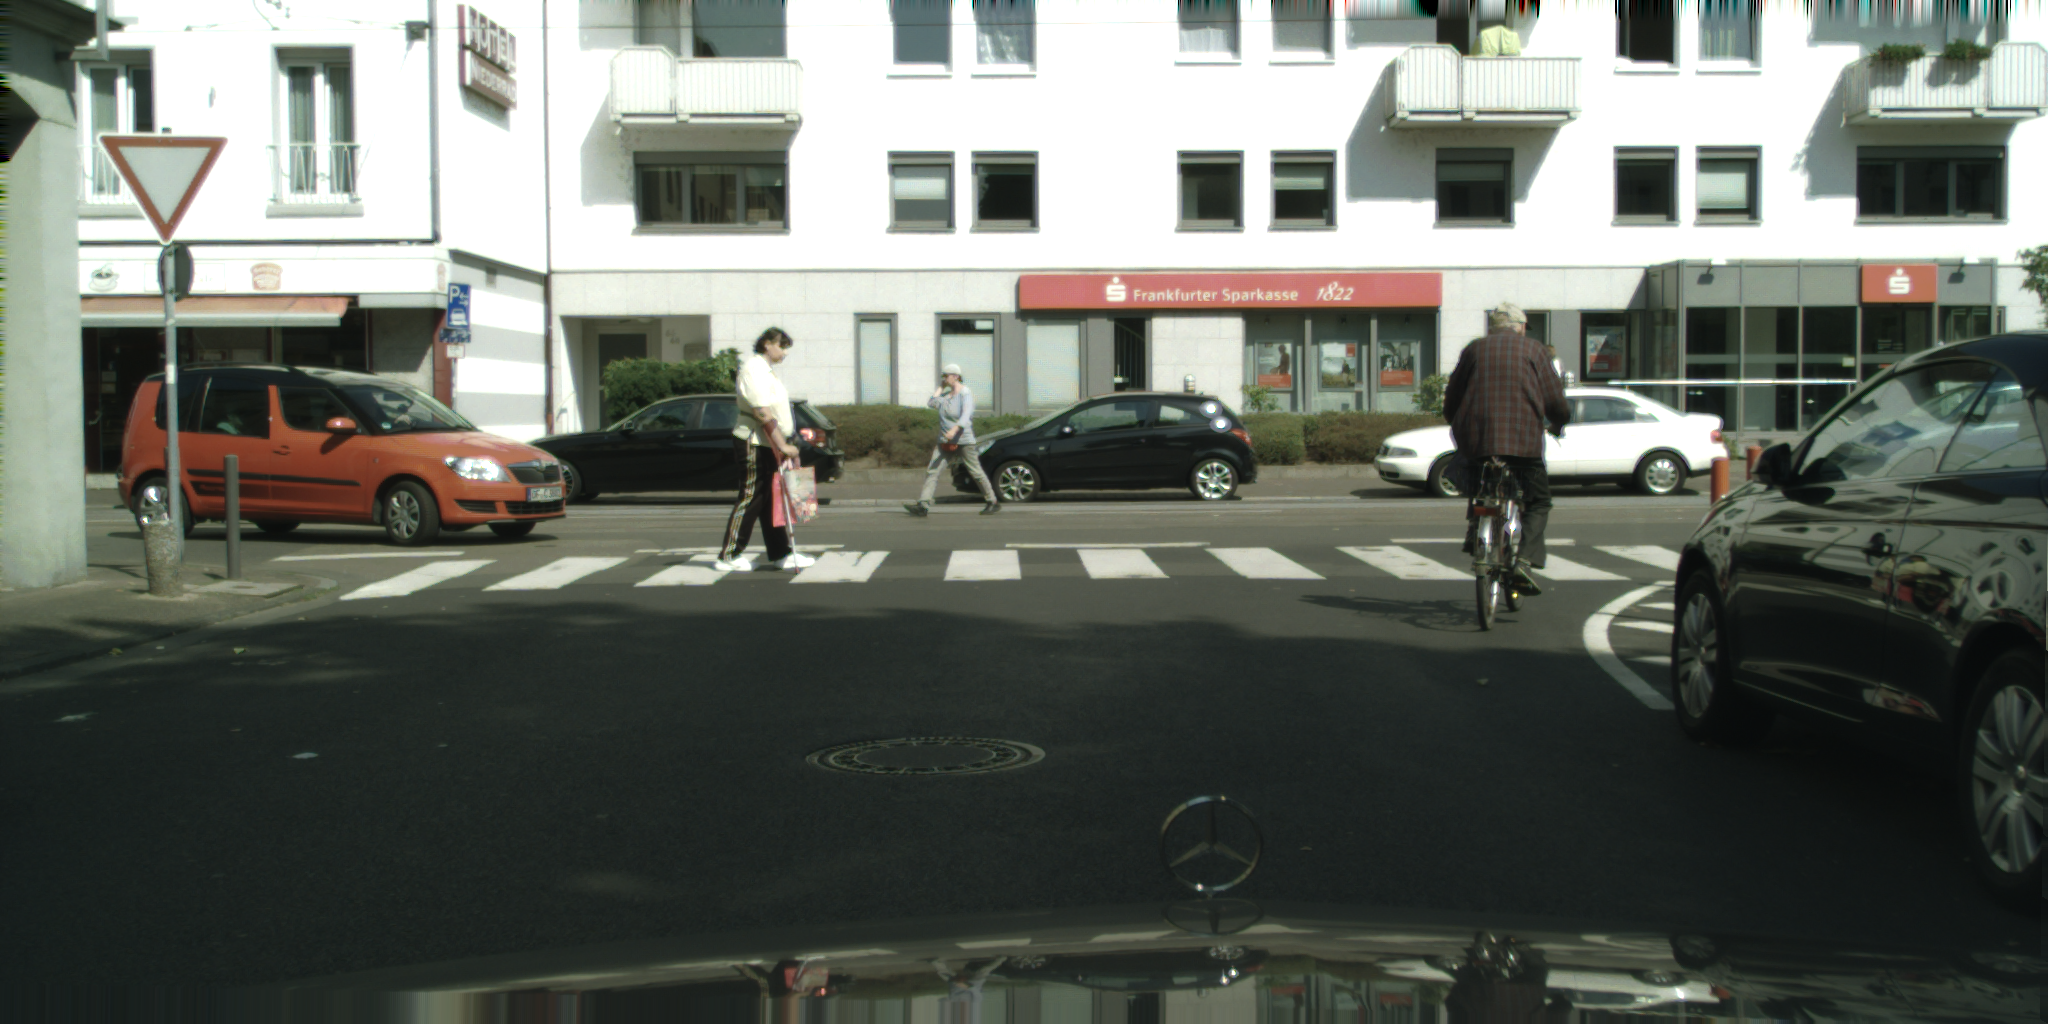
\includegraphics[width=.3\linewidth]{res/lightweight-uda-baseline-qualitative/image.png}                     & 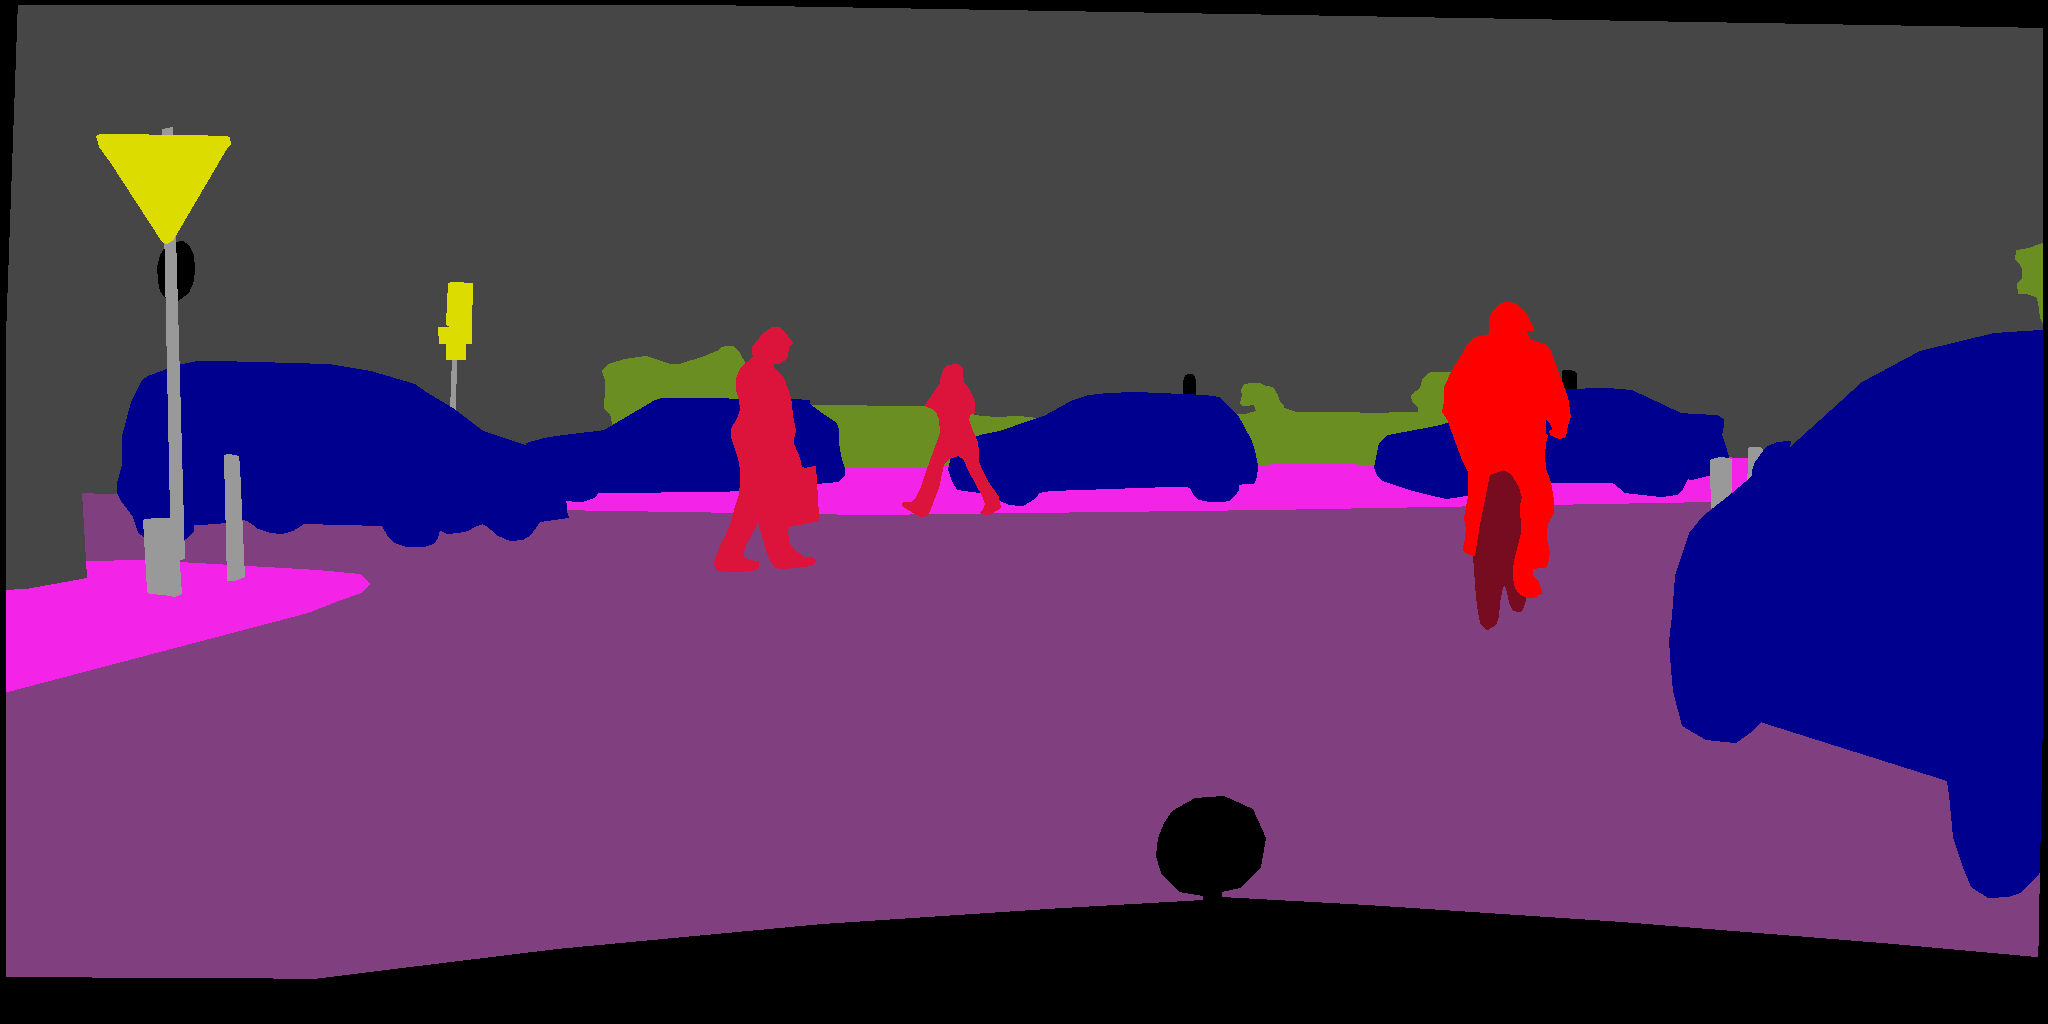
\includegraphics[width=.3\linewidth]{res/lightweight-uda-baseline-qualitative/ground-truth.png}                \\
            \textbf{Model} & \textbf{Source-Only}                                                                                         & \textbf{Self-Training}                                                                                         \\
            Topformer-Base & 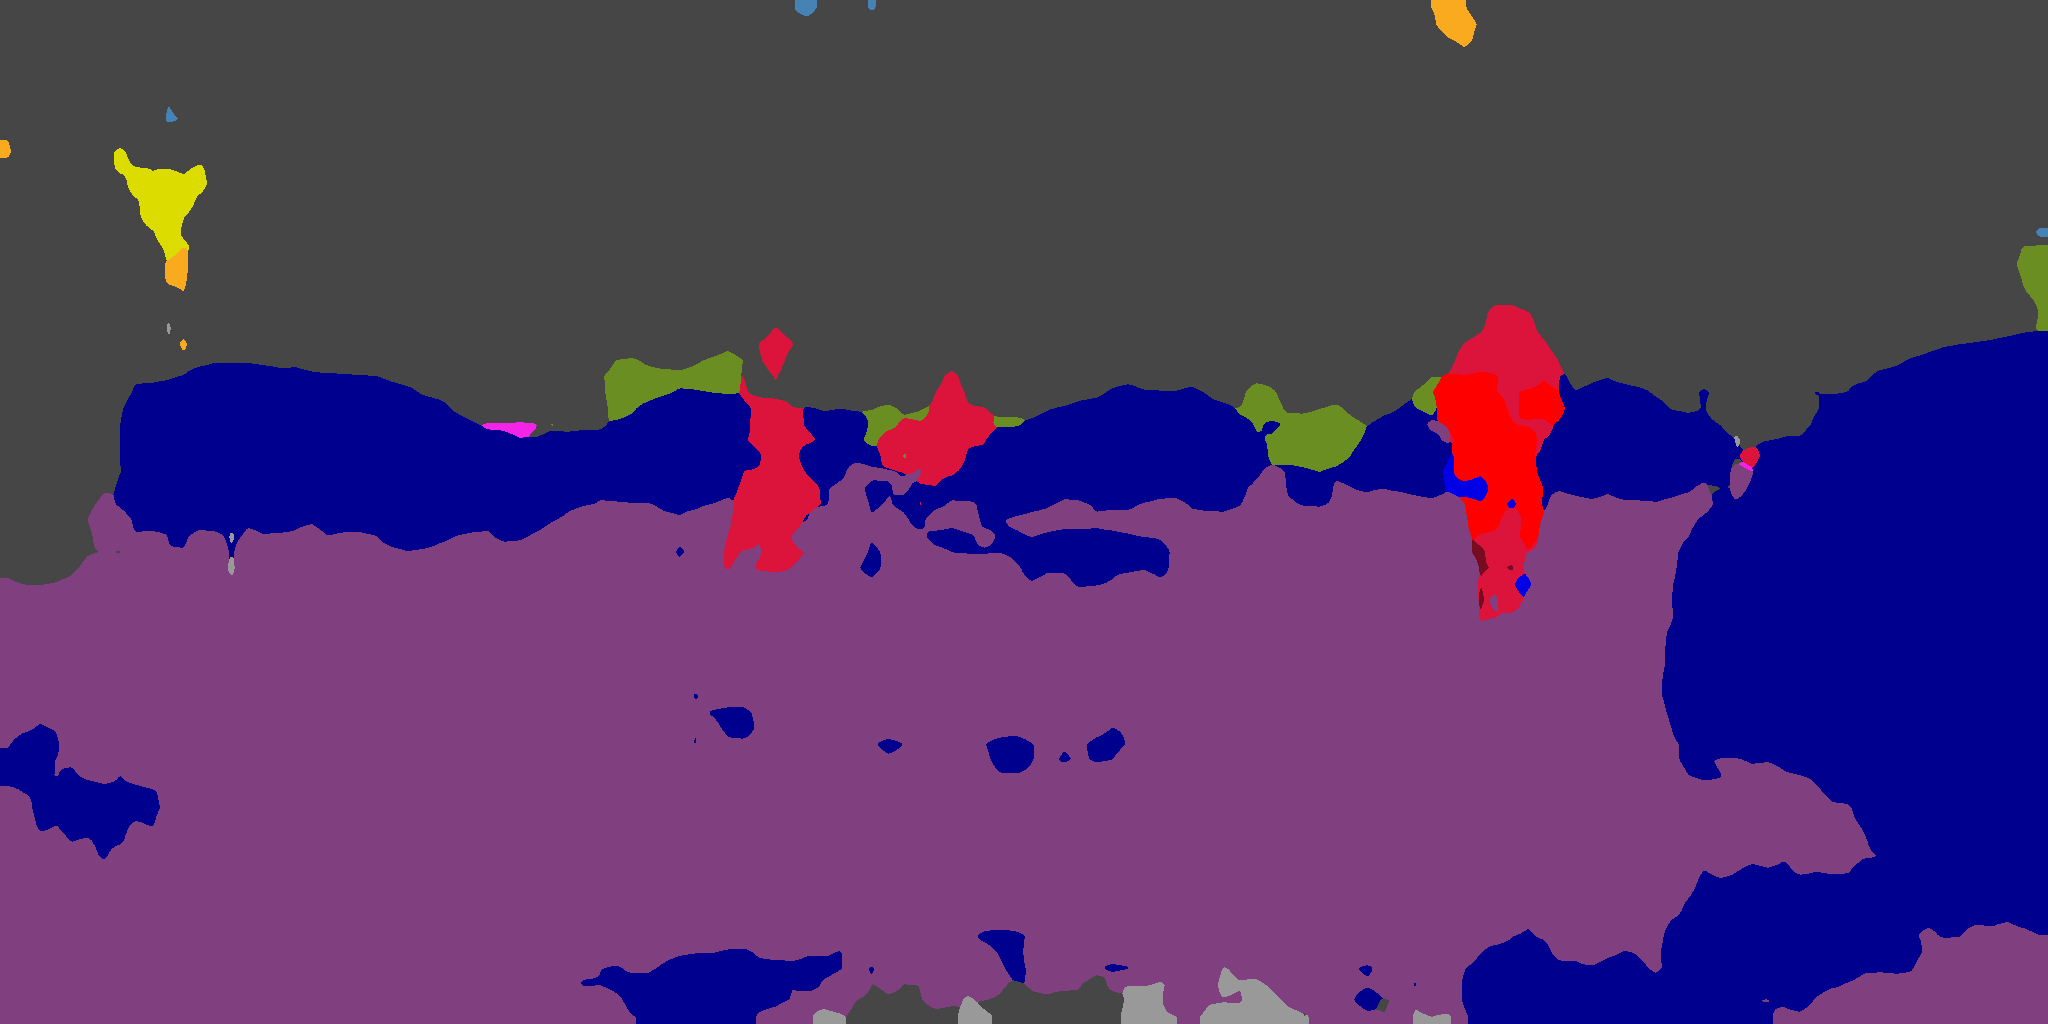
\includegraphics[width=.3\linewidth]{res/lightweight-uda-baseline-qualitative/topformer-base-sourceonly.png} & 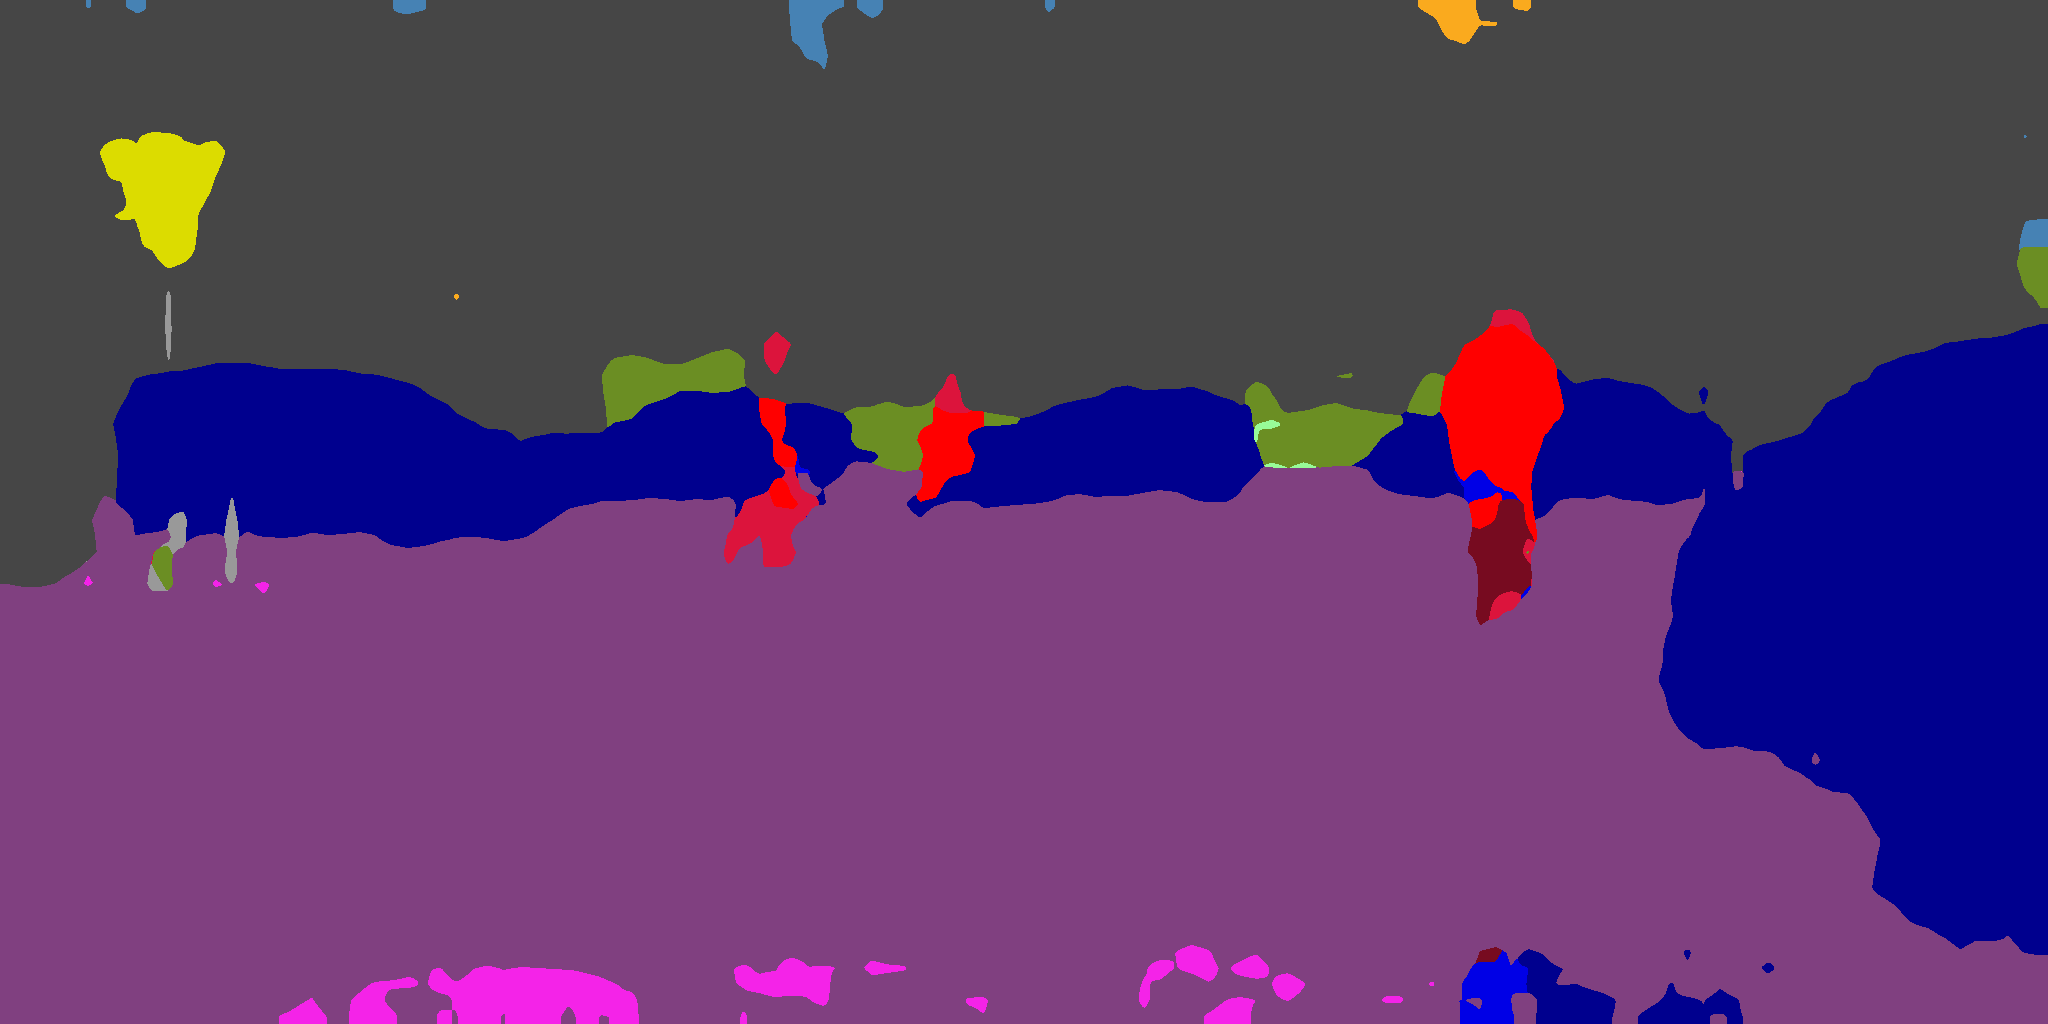
\includegraphics[width=.3\linewidth]{res/lightweight-uda-baseline-qualitative/topformer-base-selftraining.png} \\
            Topformer-Tiny & 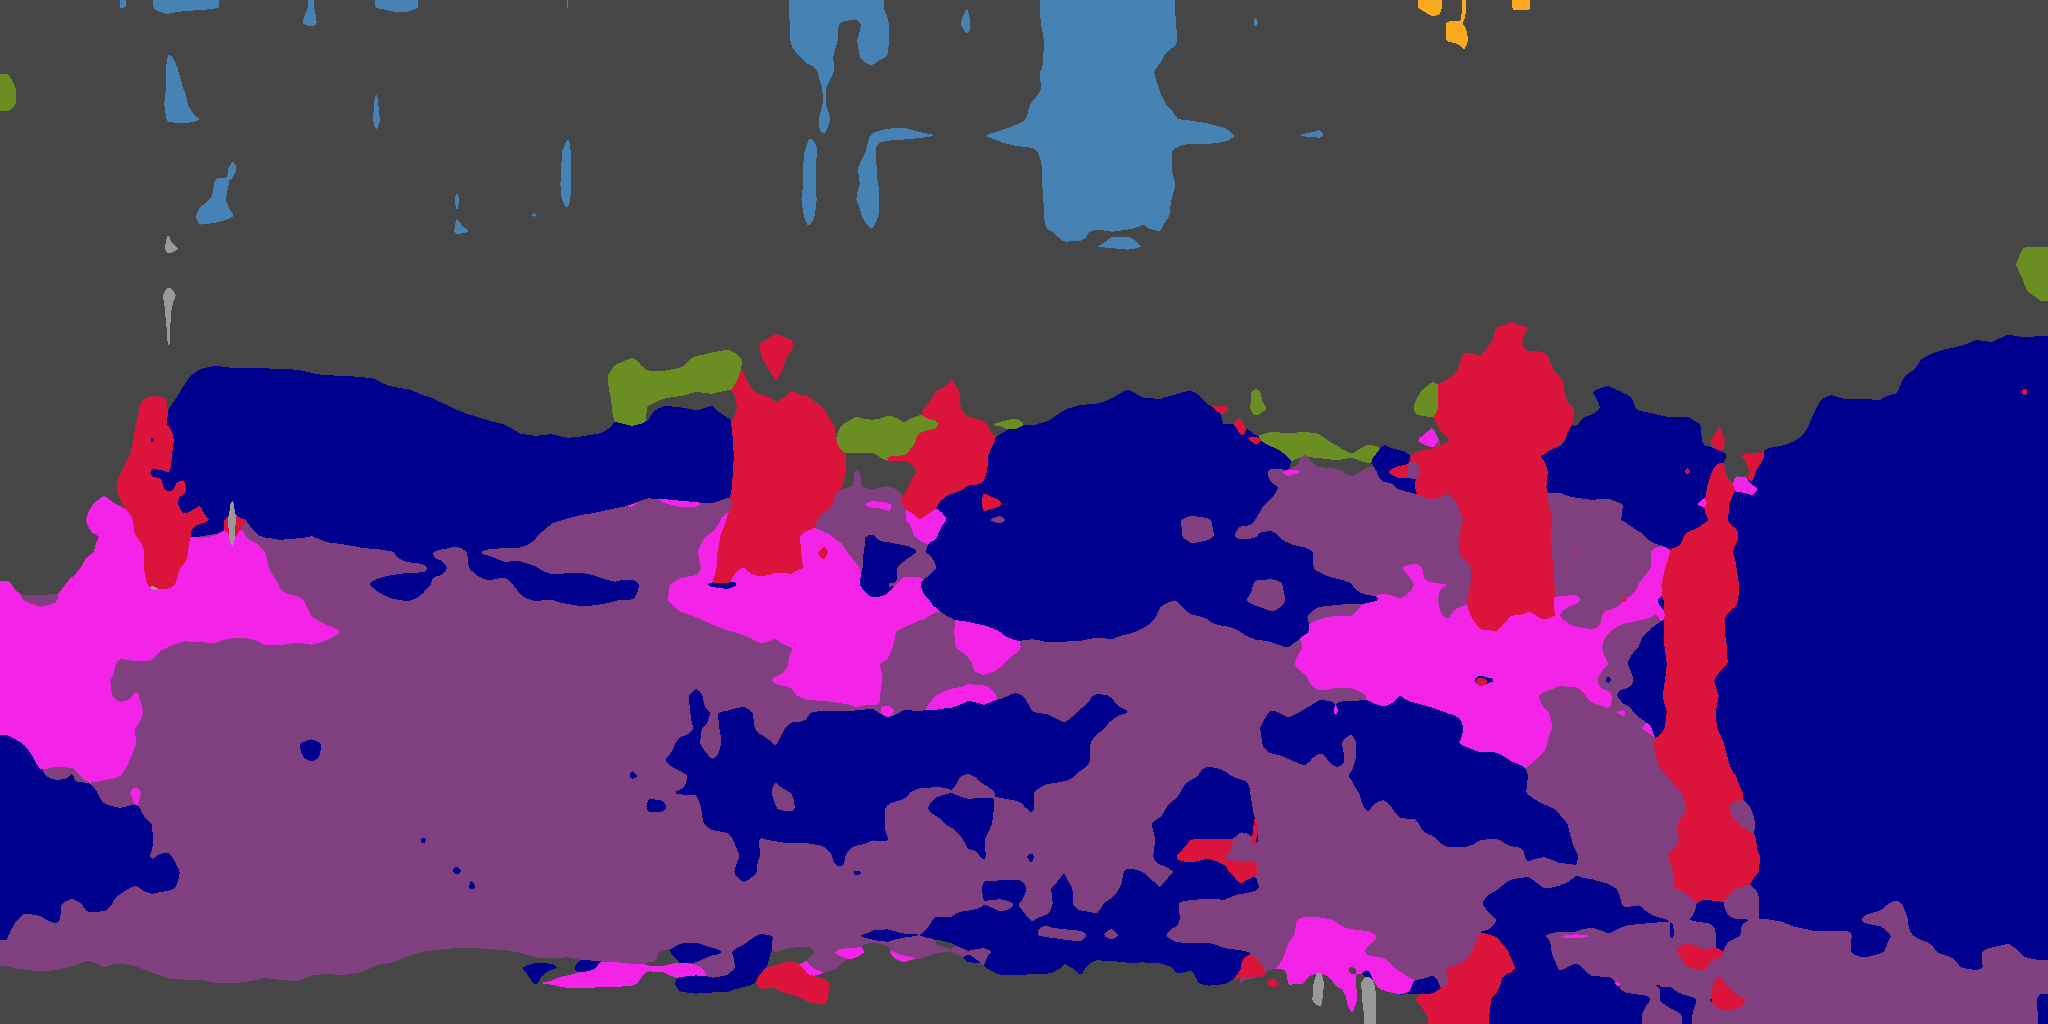
\includegraphics[width=.3\linewidth]{res/lightweight-uda-baseline-qualitative/topformer-tiny-sourceonly.png} & 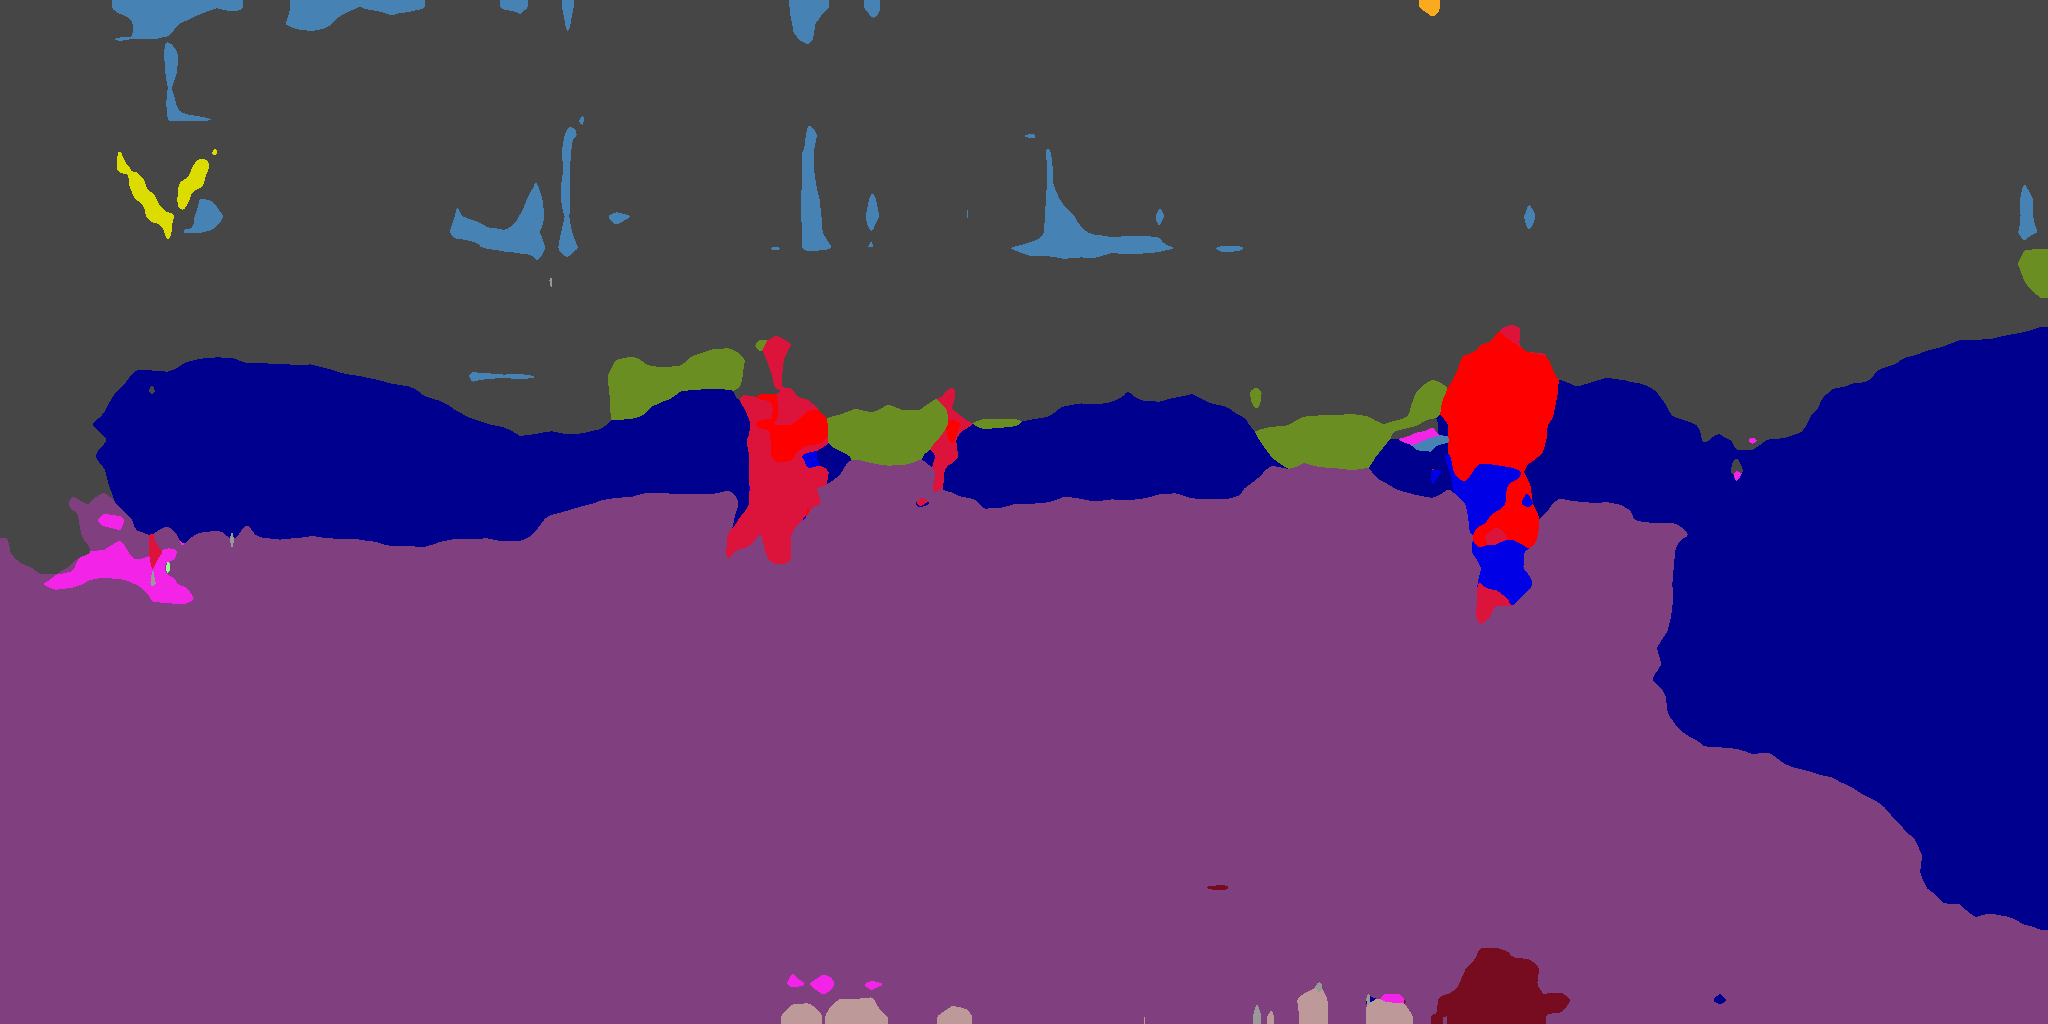
\includegraphics[width=.3\linewidth]{res/lightweight-uda-baseline-qualitative/topformer-tiny-selftraining.png} \\
        \end{tabular}
        % }
        % \caption{Qualitative baseline experiment results.}
        % \label{fig: lightweight-model-baseline}
    \end{figure}
\end{frame}


\begin{frame}{Baseline Qualitative Comparison}
    \begin{figure}[]
        % \resizebox{\textwidth}{!}{%
        \centering
        \begin{tabular}{lll}
            MobileViT-Small    & 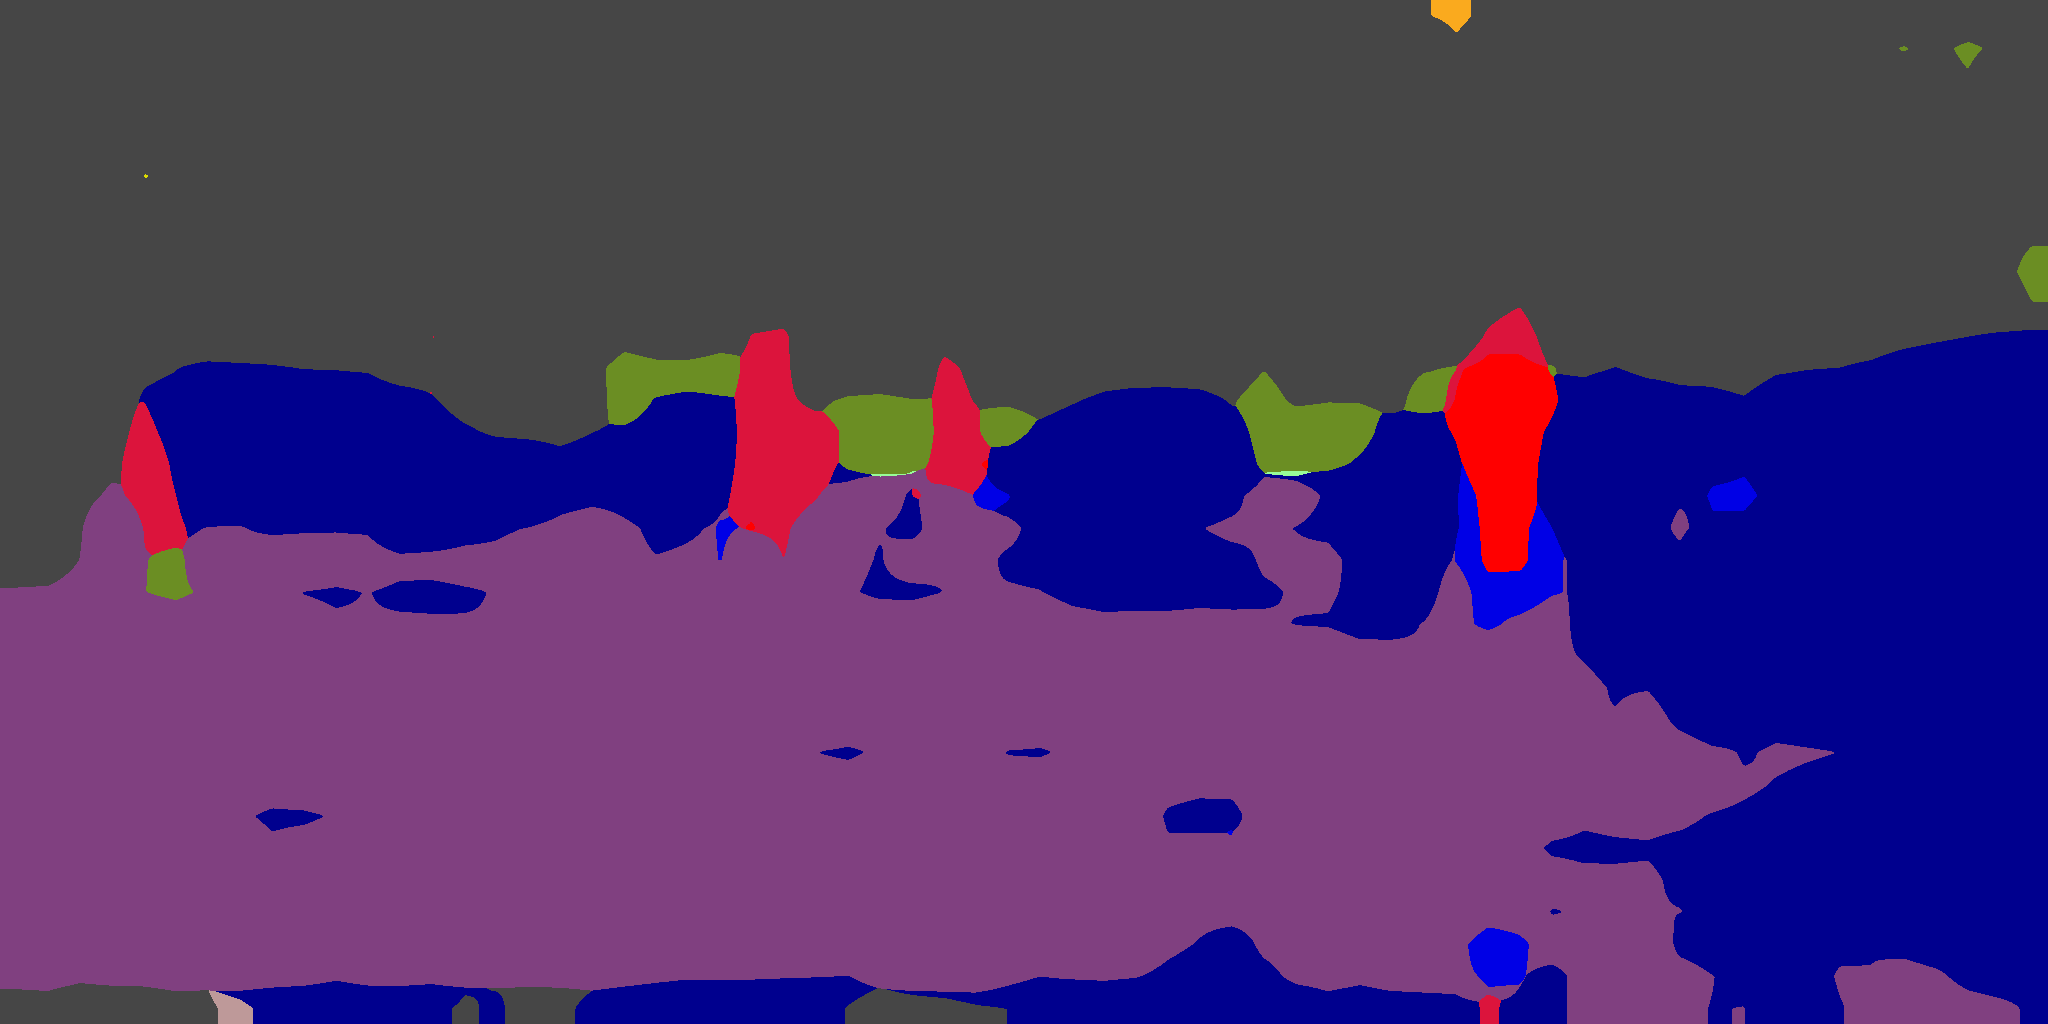
\includegraphics[width=.3\linewidth]{res/lightweight-uda-baseline-qualitative/mobilevit-small-sourceonly.png}    & 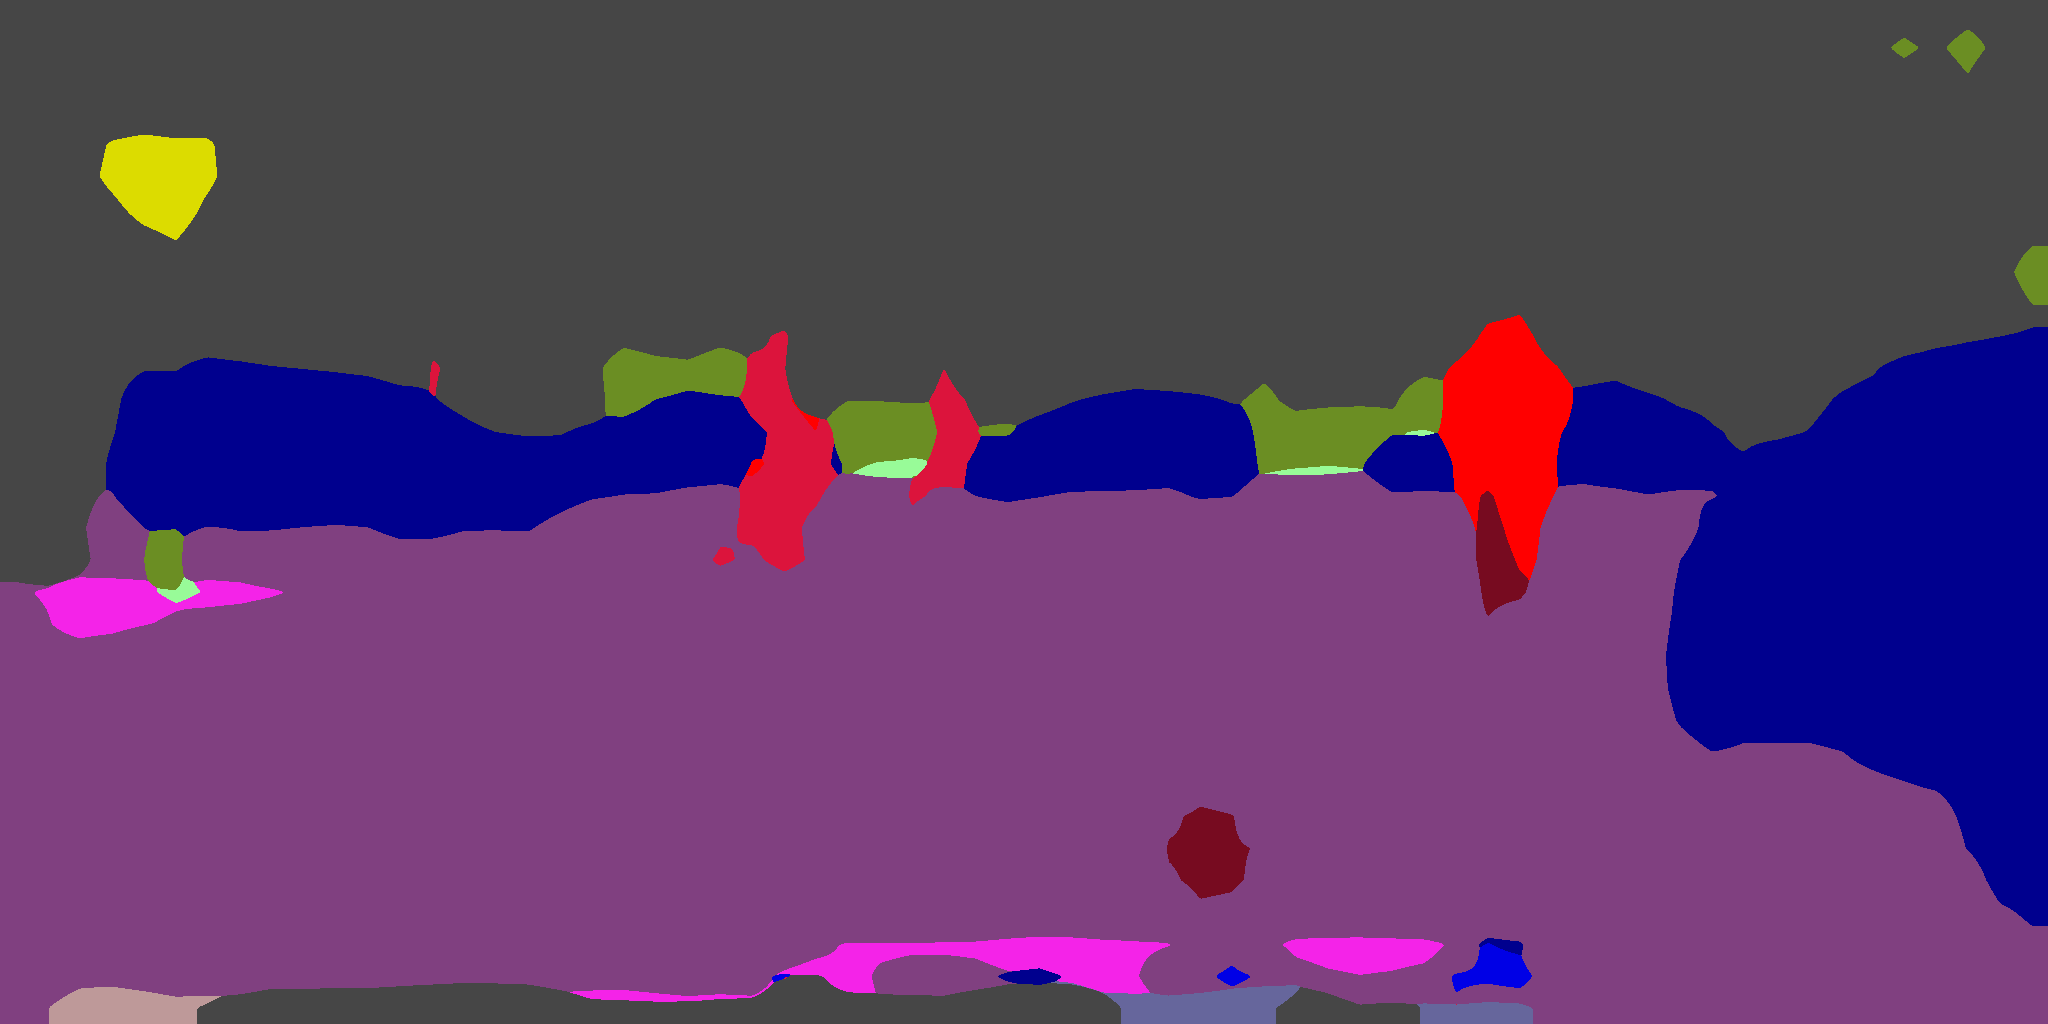
\includegraphics[width=.3\linewidth]{res/lightweight-uda-baseline-qualitative/mobilevit-small-selftraining.png}    \\
            MobileViT-XX-Small & 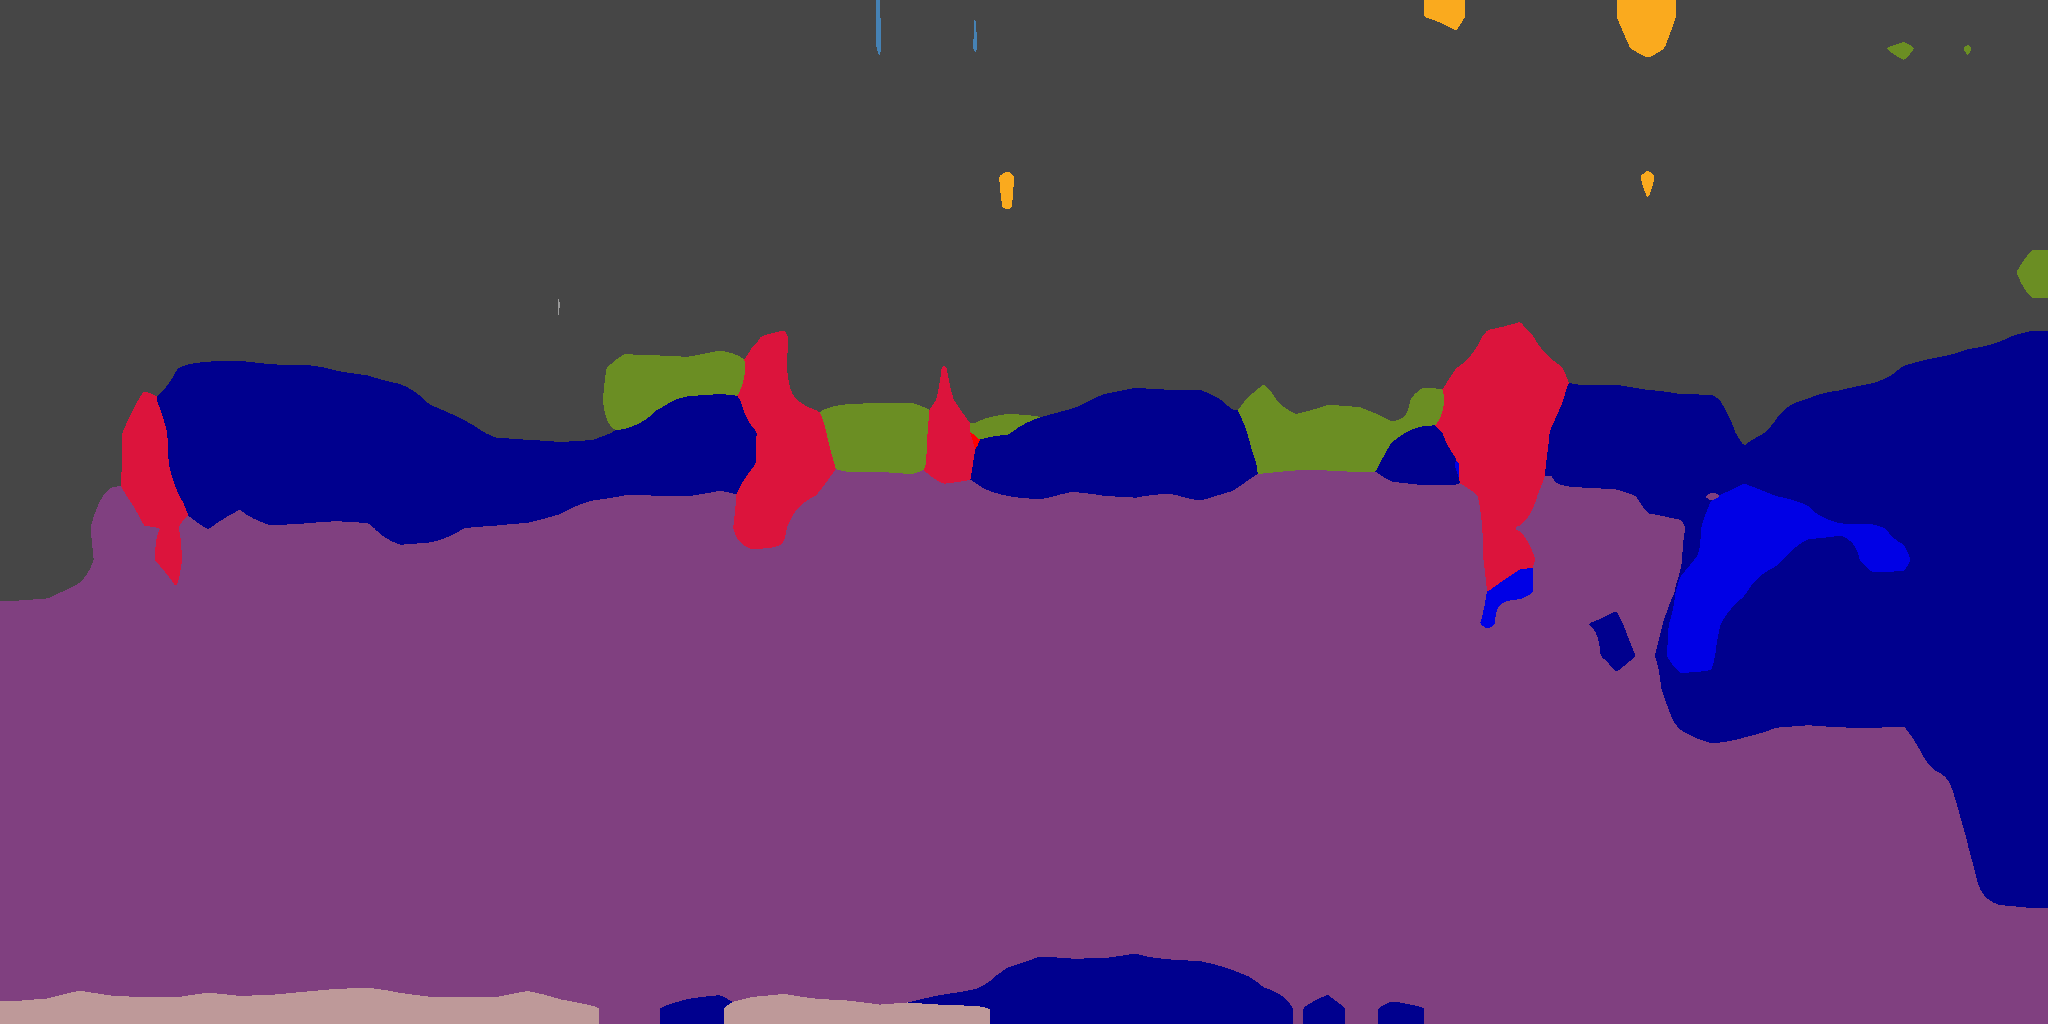
\includegraphics[width=.3\linewidth]{res/lightweight-uda-baseline-qualitative/mobilevit-xx-small-sourceonly.png} & 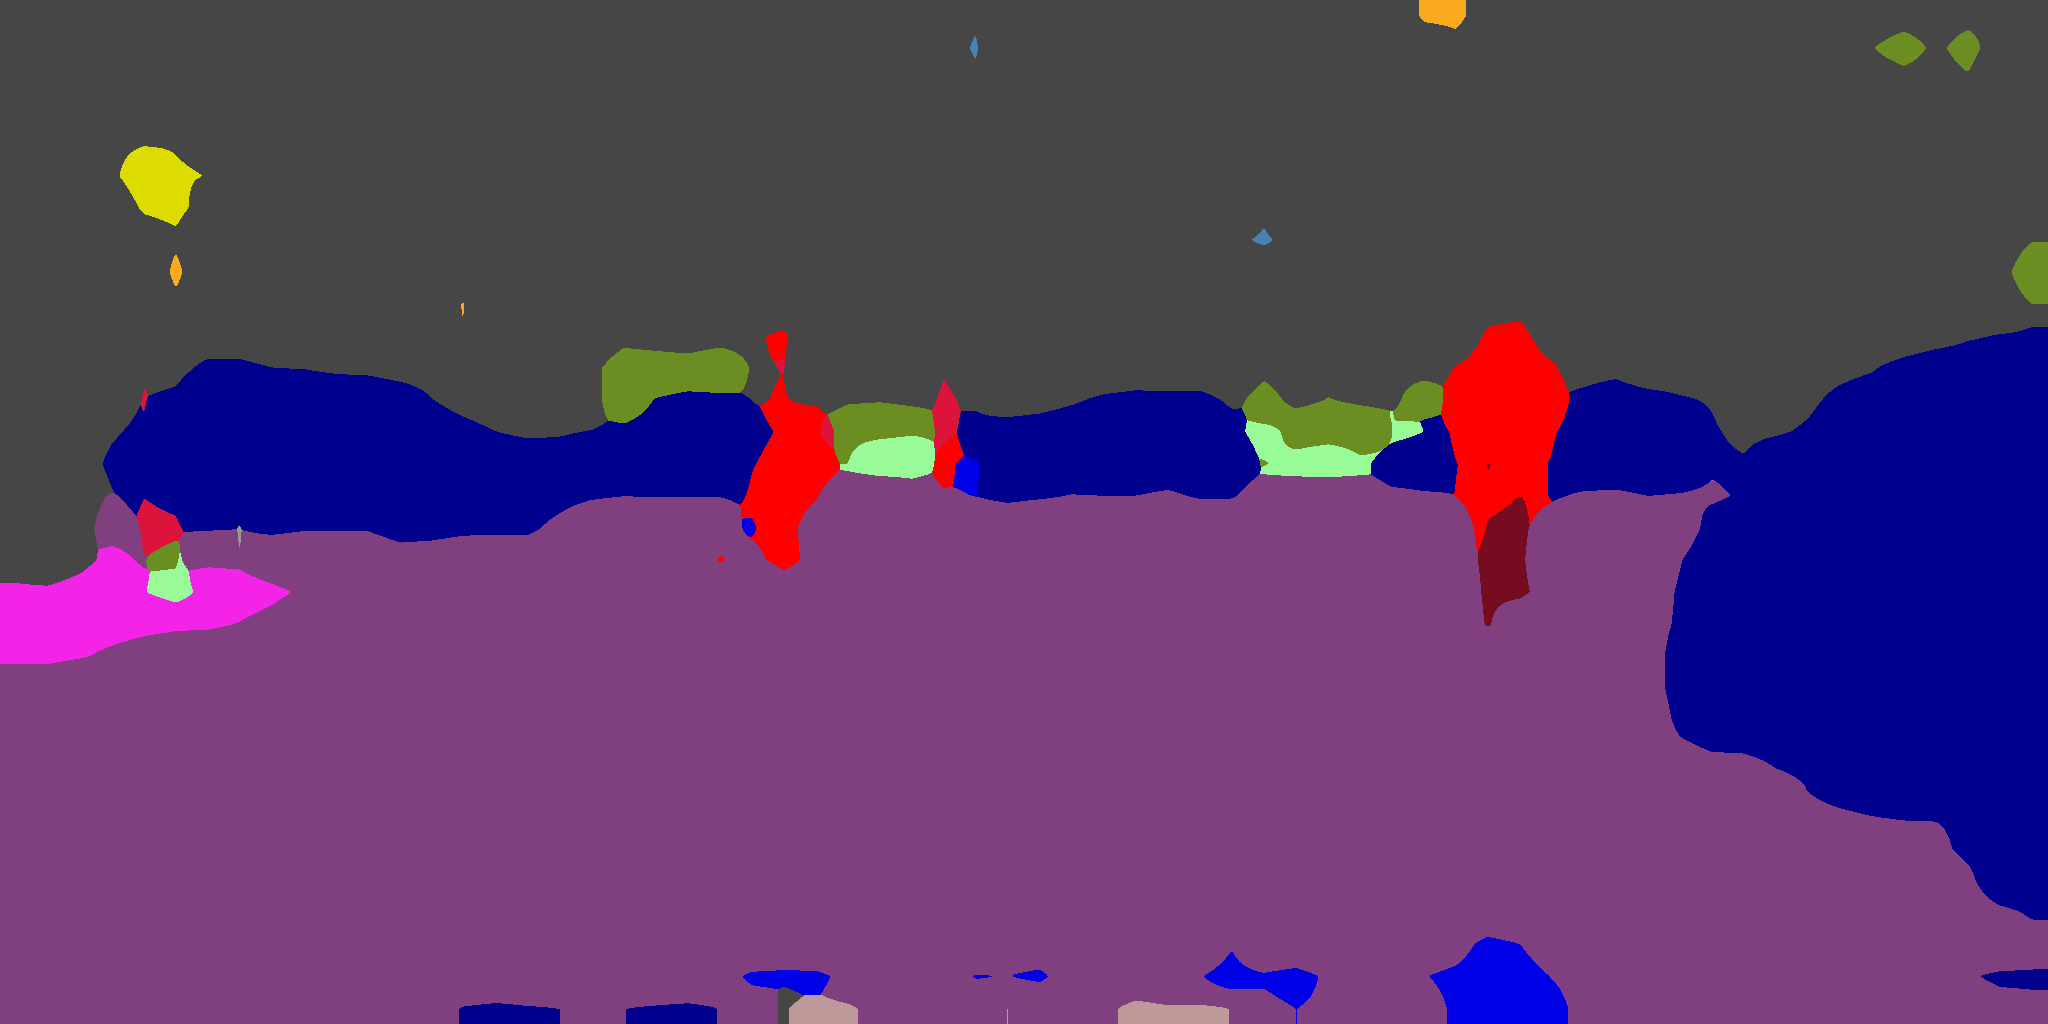
\includegraphics[width=.3\linewidth]{res/lightweight-uda-baseline-qualitative/mobilevit-xx-small-selftraining.png} \\
            Fast-SCNN          & 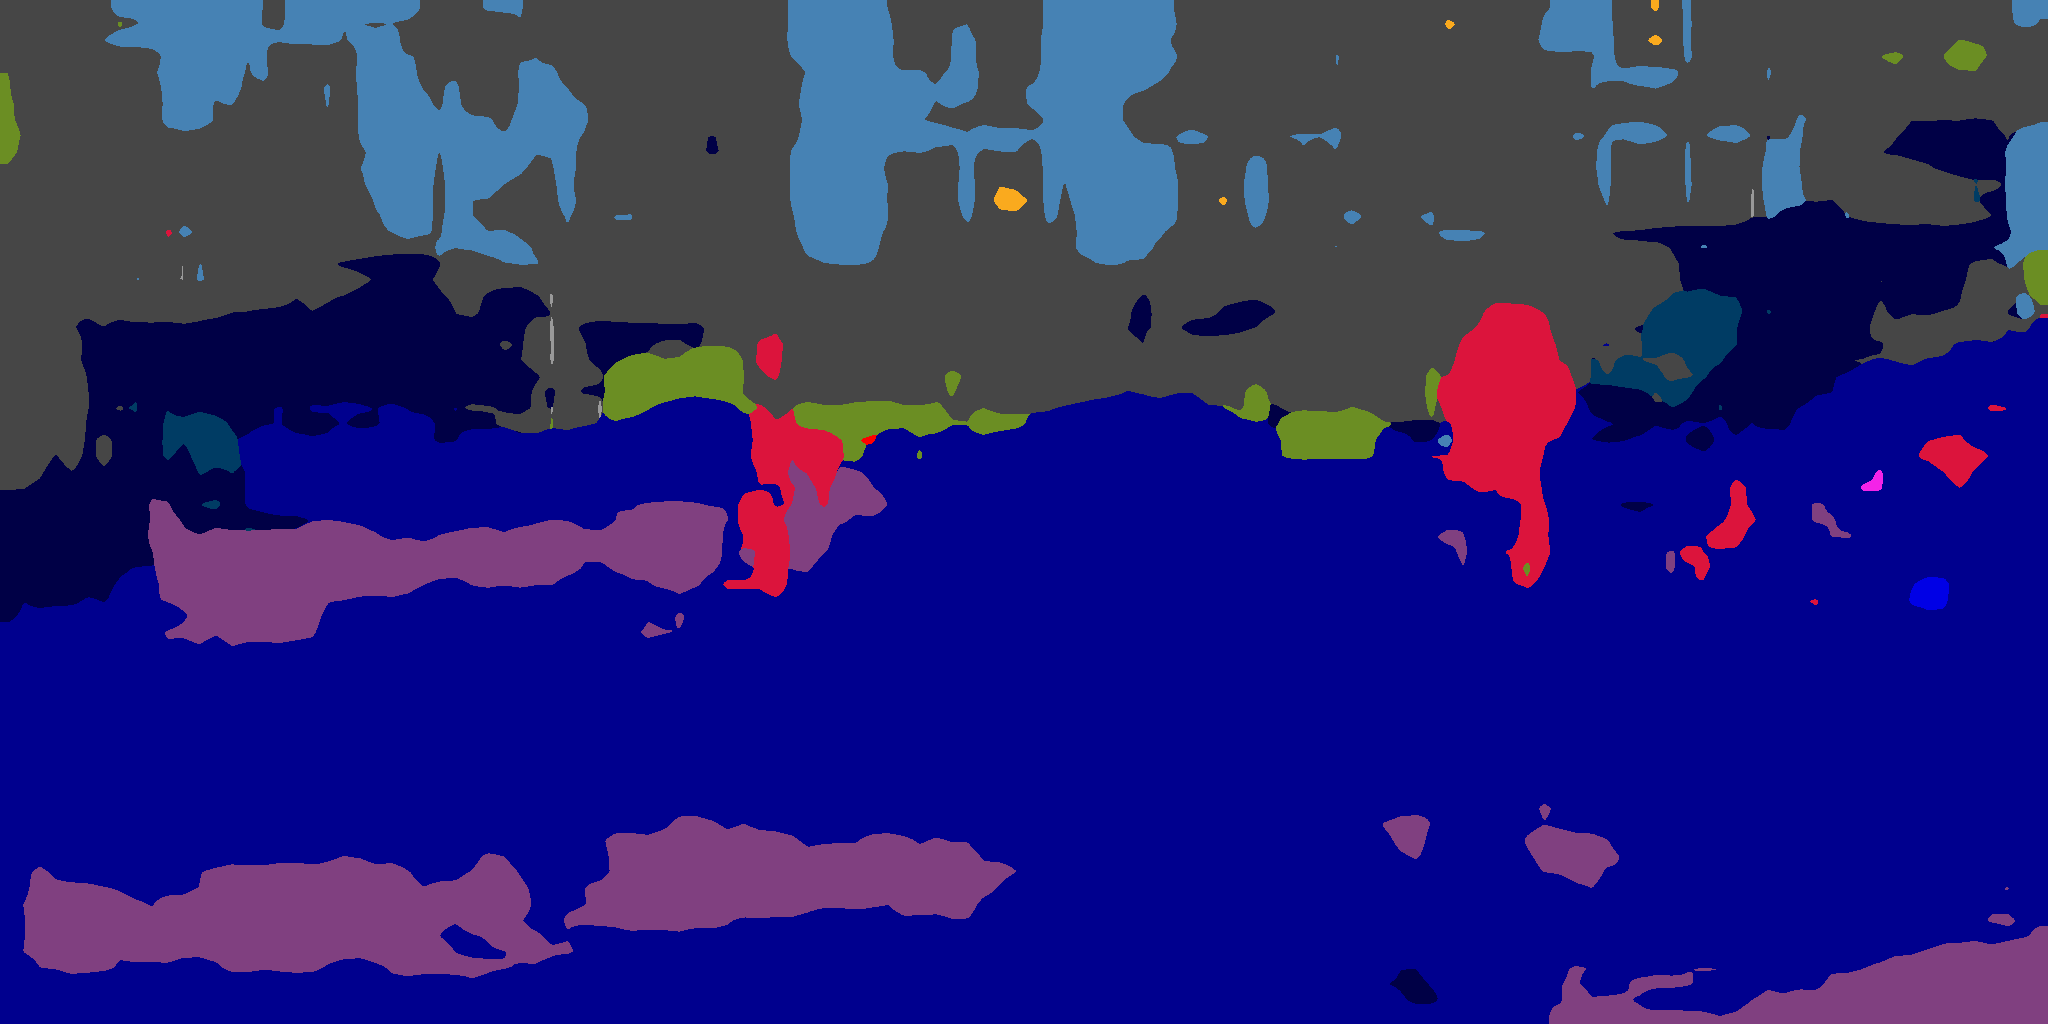
\includegraphics[width=.3\linewidth]{res/lightweight-uda-baseline-qualitative/fast-scnn-sourceonly.png}          & N/A                                                                                                                \\
        \end{tabular}
        % }
        % \caption{Qualitative baseline experiment results.}
        % \label{fig: lightweight-model-baseline}
    \end{figure}
\end{frame}

\begin{frame}{Baseline Qualitative Comparison}
    \begin{figure}[]
        % \resizebox{\textwidth}{!}{%
        \centering
        \begin{tabular}{lll}
            SegFormer-B0 & 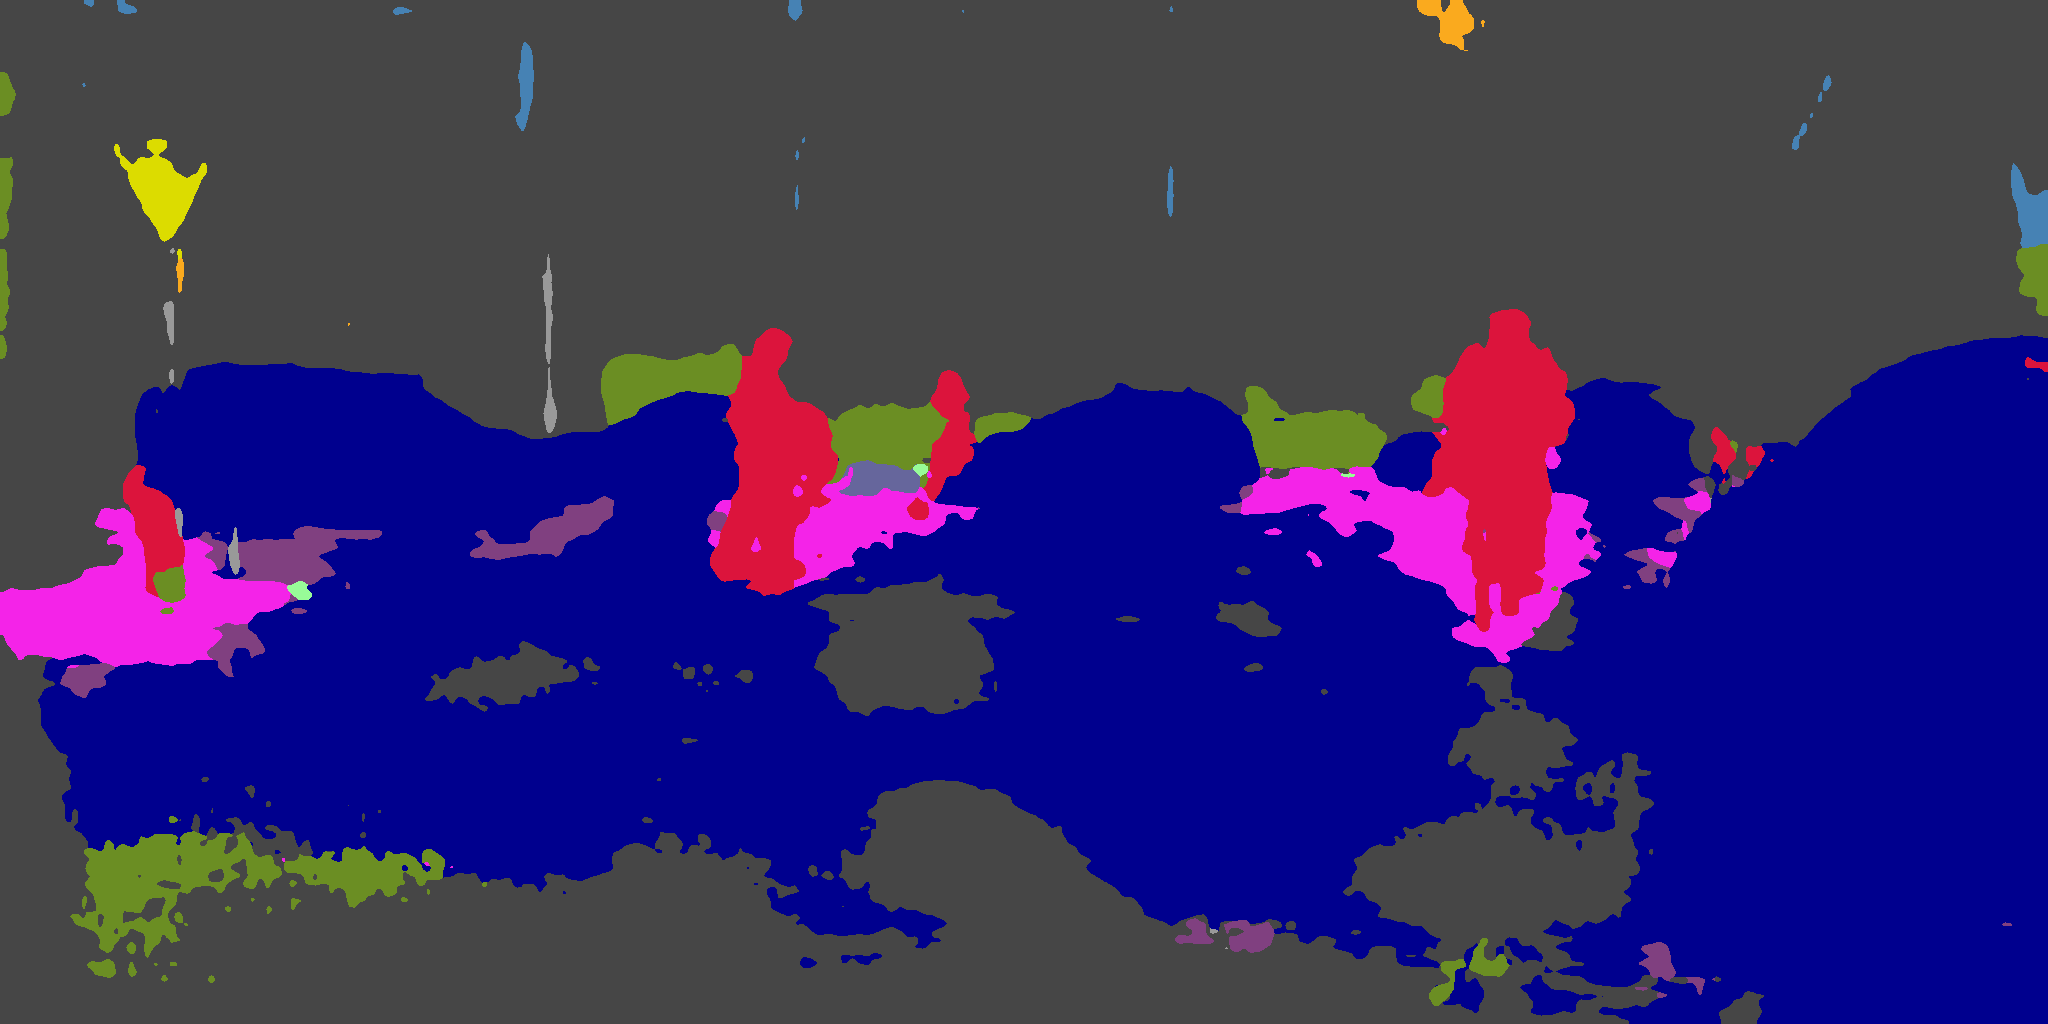
\includegraphics[width=.3\linewidth]{res/lightweight-uda-baseline-qualitative/segformer-mitb0-sourceonly.png} & 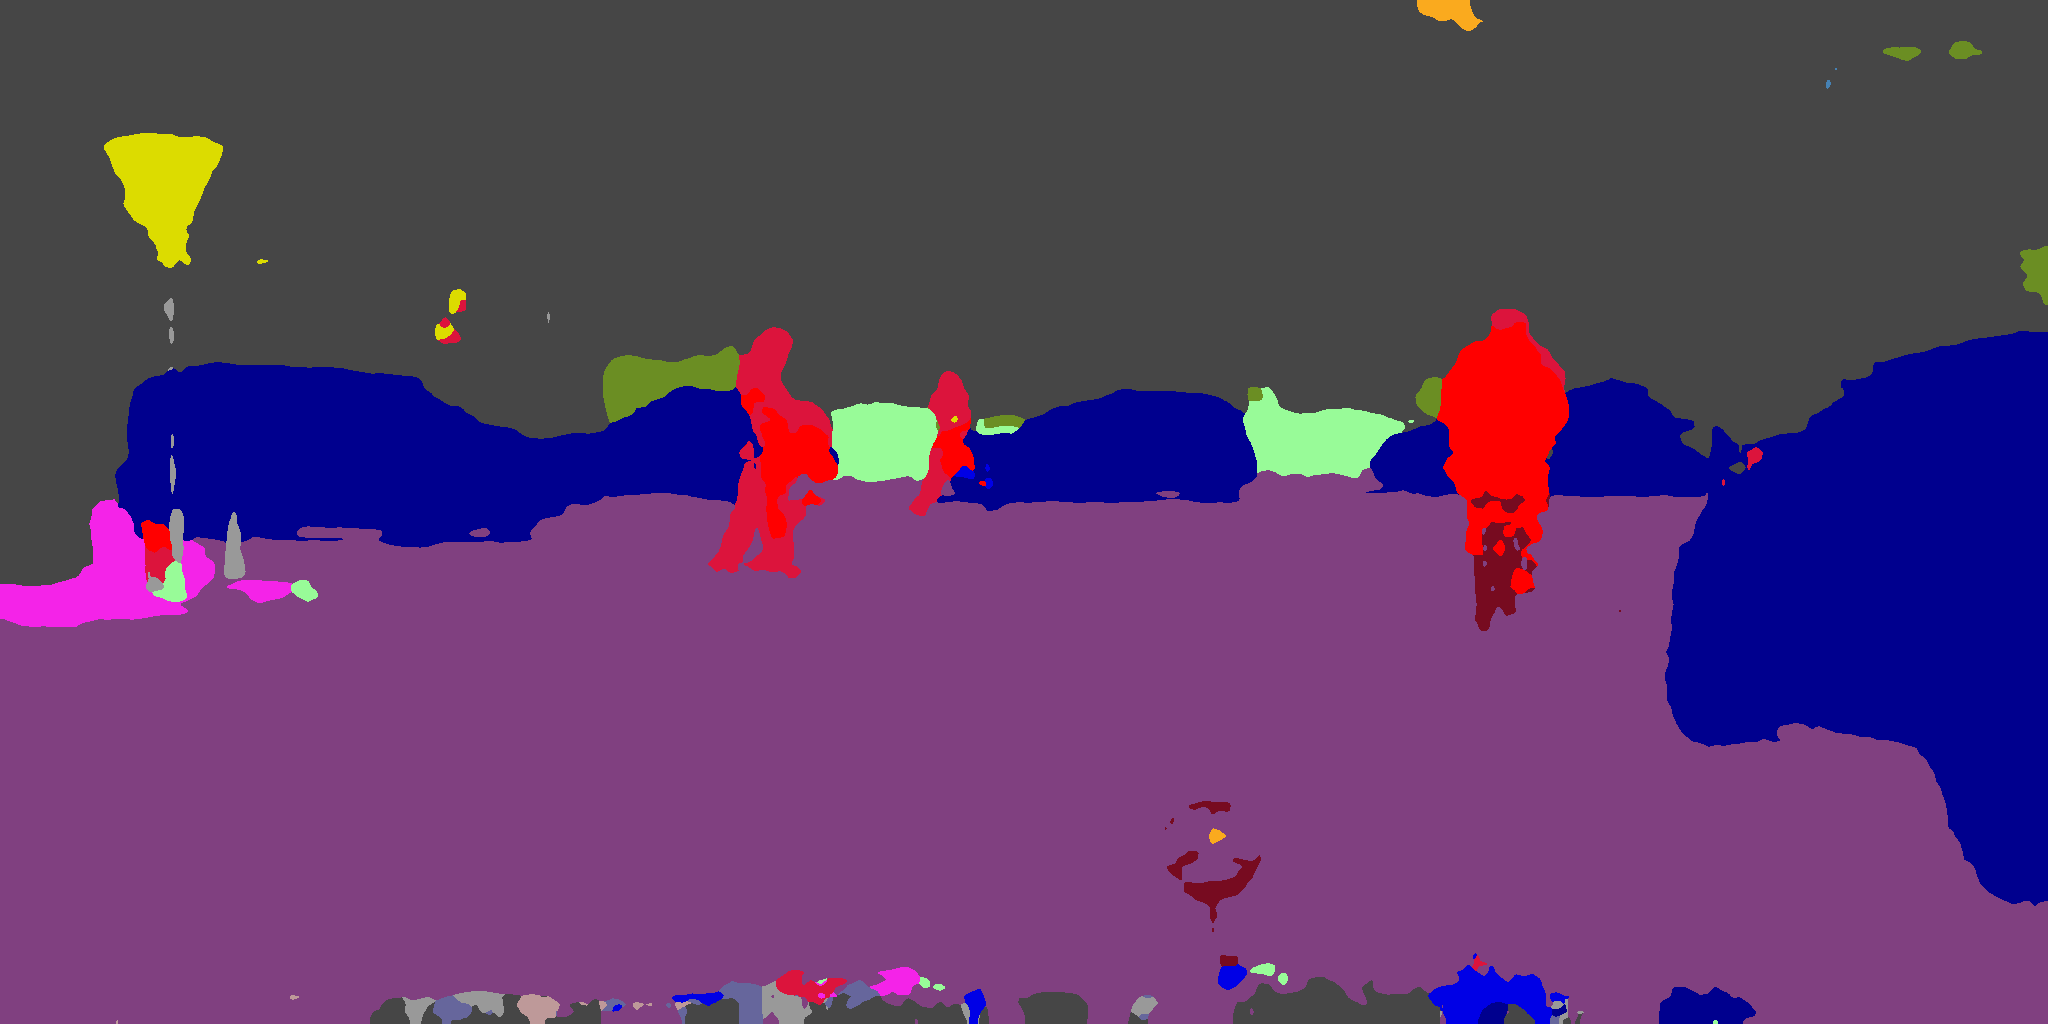
\includegraphics[width=.3\linewidth]{res/lightweight-uda-baseline-qualitative/segformer-mitb0-selftraining.png} \\
            DAFormer-B0  & 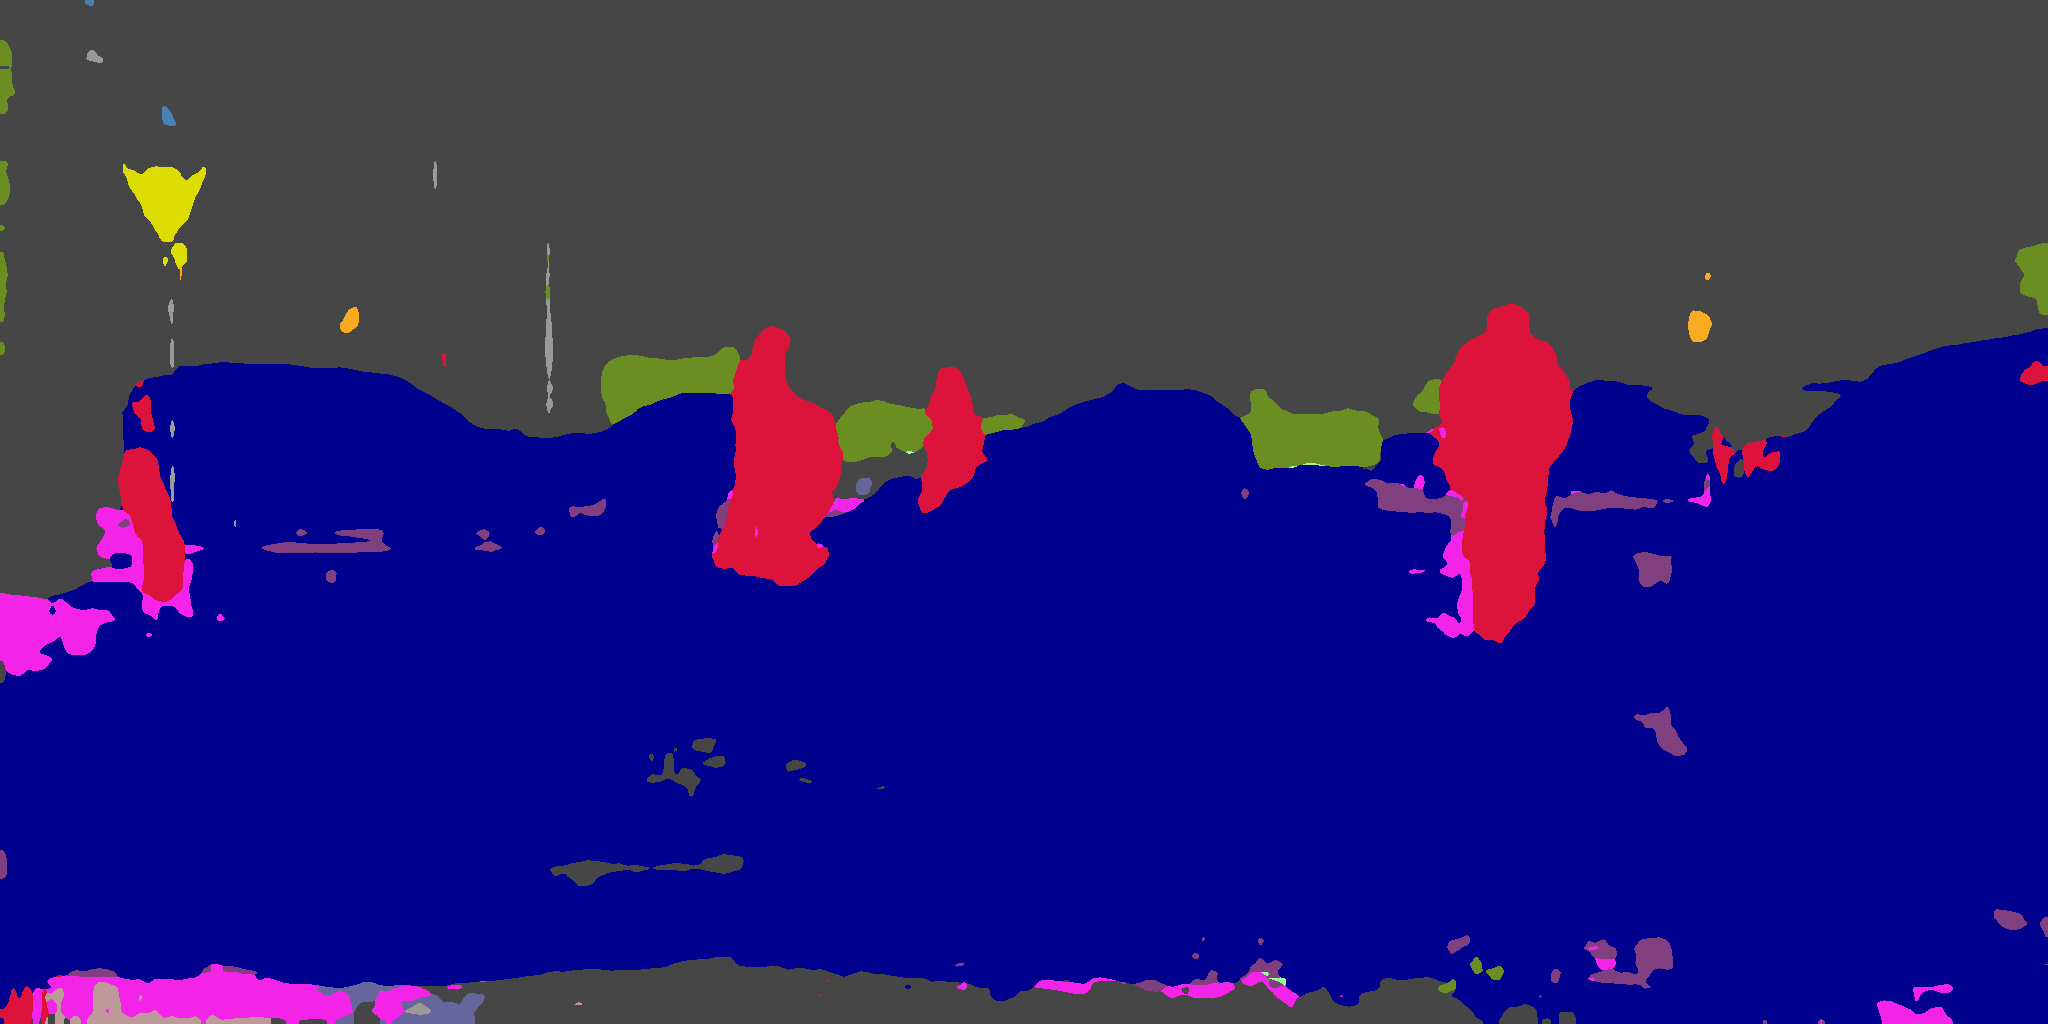
\includegraphics[width=.3\linewidth]{res/lightweight-uda-baseline-qualitative/daformer-mitb0-sourceonly.png}  & 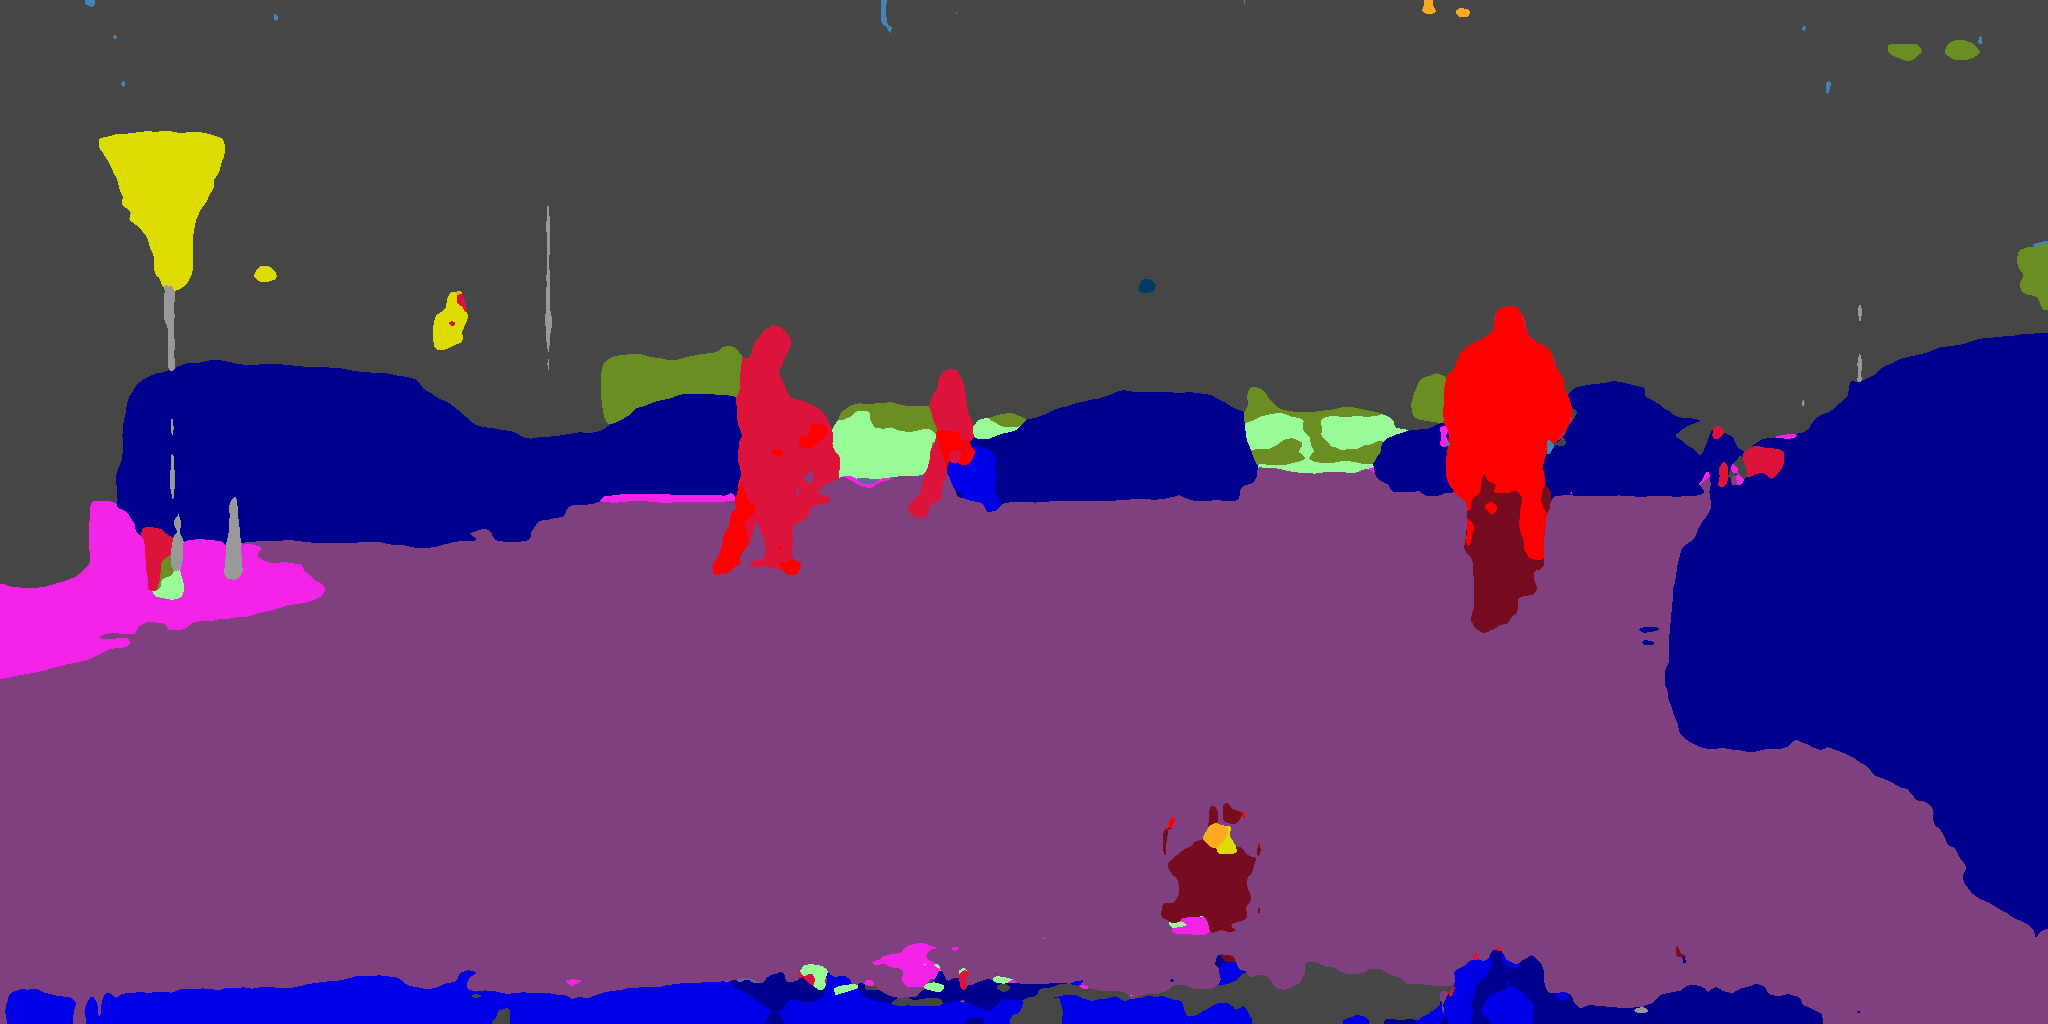
\includegraphics[width=.3\linewidth]{res/lightweight-uda-baseline-qualitative/daformer-mitb0-selftraining.png}  \\
        \end{tabular}
        % }
        % \caption{Qualitative baseline experiment results.}
        % \label{fig: lightweight-model-baseline}
    \end{figure}
\end{frame}

\begin{frame}{Pseudo-Teacher UDA}
    \begin{figure}[ht]
        \centering
        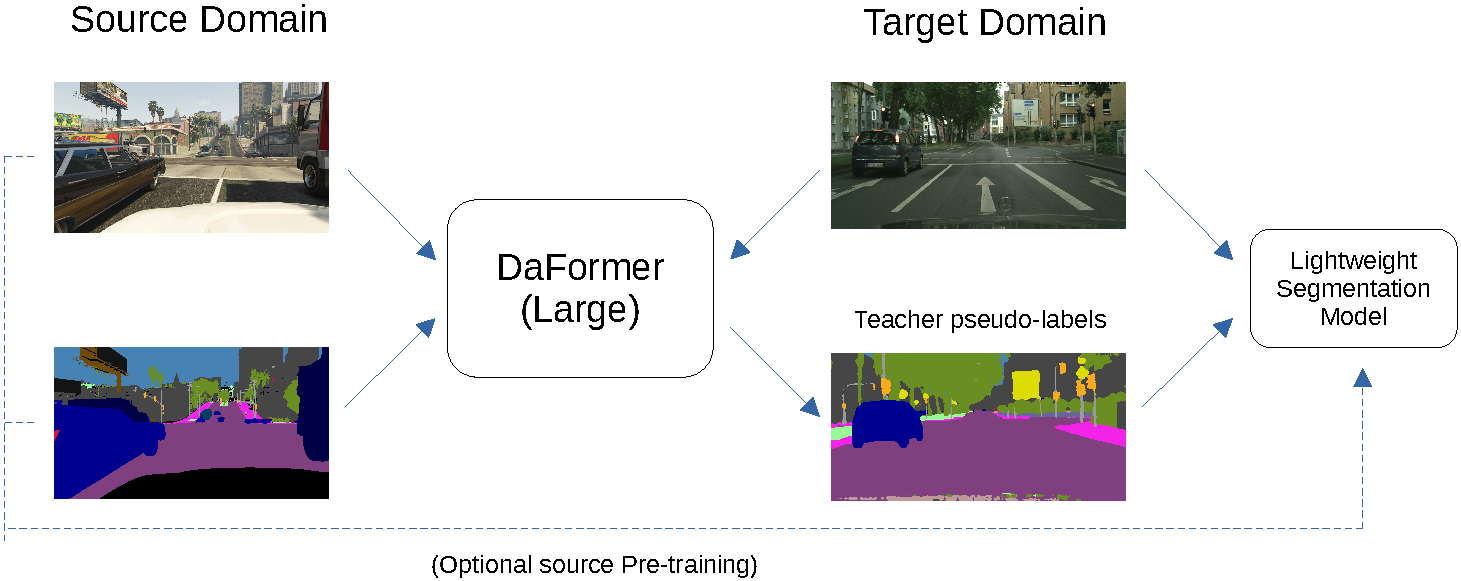
\includegraphics[width=\textwidth]{res/pseudo-teacher-pipeline.pdf}
        \caption{The pseudo-teacher pipeline.}
        \label{fig:pseudo-teacher-pipeline}
    \end{figure}
\end{frame}

\begin{frame}{Pseudo-Teacher UDA Results (GTA Dataset)}
    \begin{table}[h]
        \resizebox{\textwidth}{!}{%
            \begin{tabular}{|l|l|r|r|r|r|}
                \hline
                Model             & UDA Approach   & \multicolumn{1}{l|}{Source-Only} & \multicolumn{1}{l|}{With UDA} & \multicolumn{1}{l|}{Oracle} & \multicolumn{1}{l|}{\begin{tabular}[c]{@{}l@{}}Relative \\ Performance\end{tabular}} \\ \hline
                TopFormer-Base    & Pseudo-Teacher & \textbf{33.32}                   & \textbf{61.18}                & 66.56                       & 91.92\%                                                                              \\ \hline
                TopFormer-Tiny    & Pseudo-Teacher & 27.78                            & 56.26                         & 59.39                       & \textbf{94.73\%}                                                                     \\ \hline
                DAFormer (MiT-B0) & Self-Training  & 28.12                            & 47.55                         & \textbf{70.78}              & 67.18\%                                                                              \\ \hline
            \end{tabular}
        }
        % \caption{Results of Pseudo-Teacher UDA on GTA \textrightarrow CS. All performance values are in \% mIoU}
    \end{table}
\end{frame}

\begin{frame}{Pseudo-Teacher Qualitative Results (GTA Dataset)}
    \begin{table}[hb]
        \resizebox{\textwidth}{!}{%
            \begin{tabular}{lllll}
                \centering
                Ground Truth   &                   & 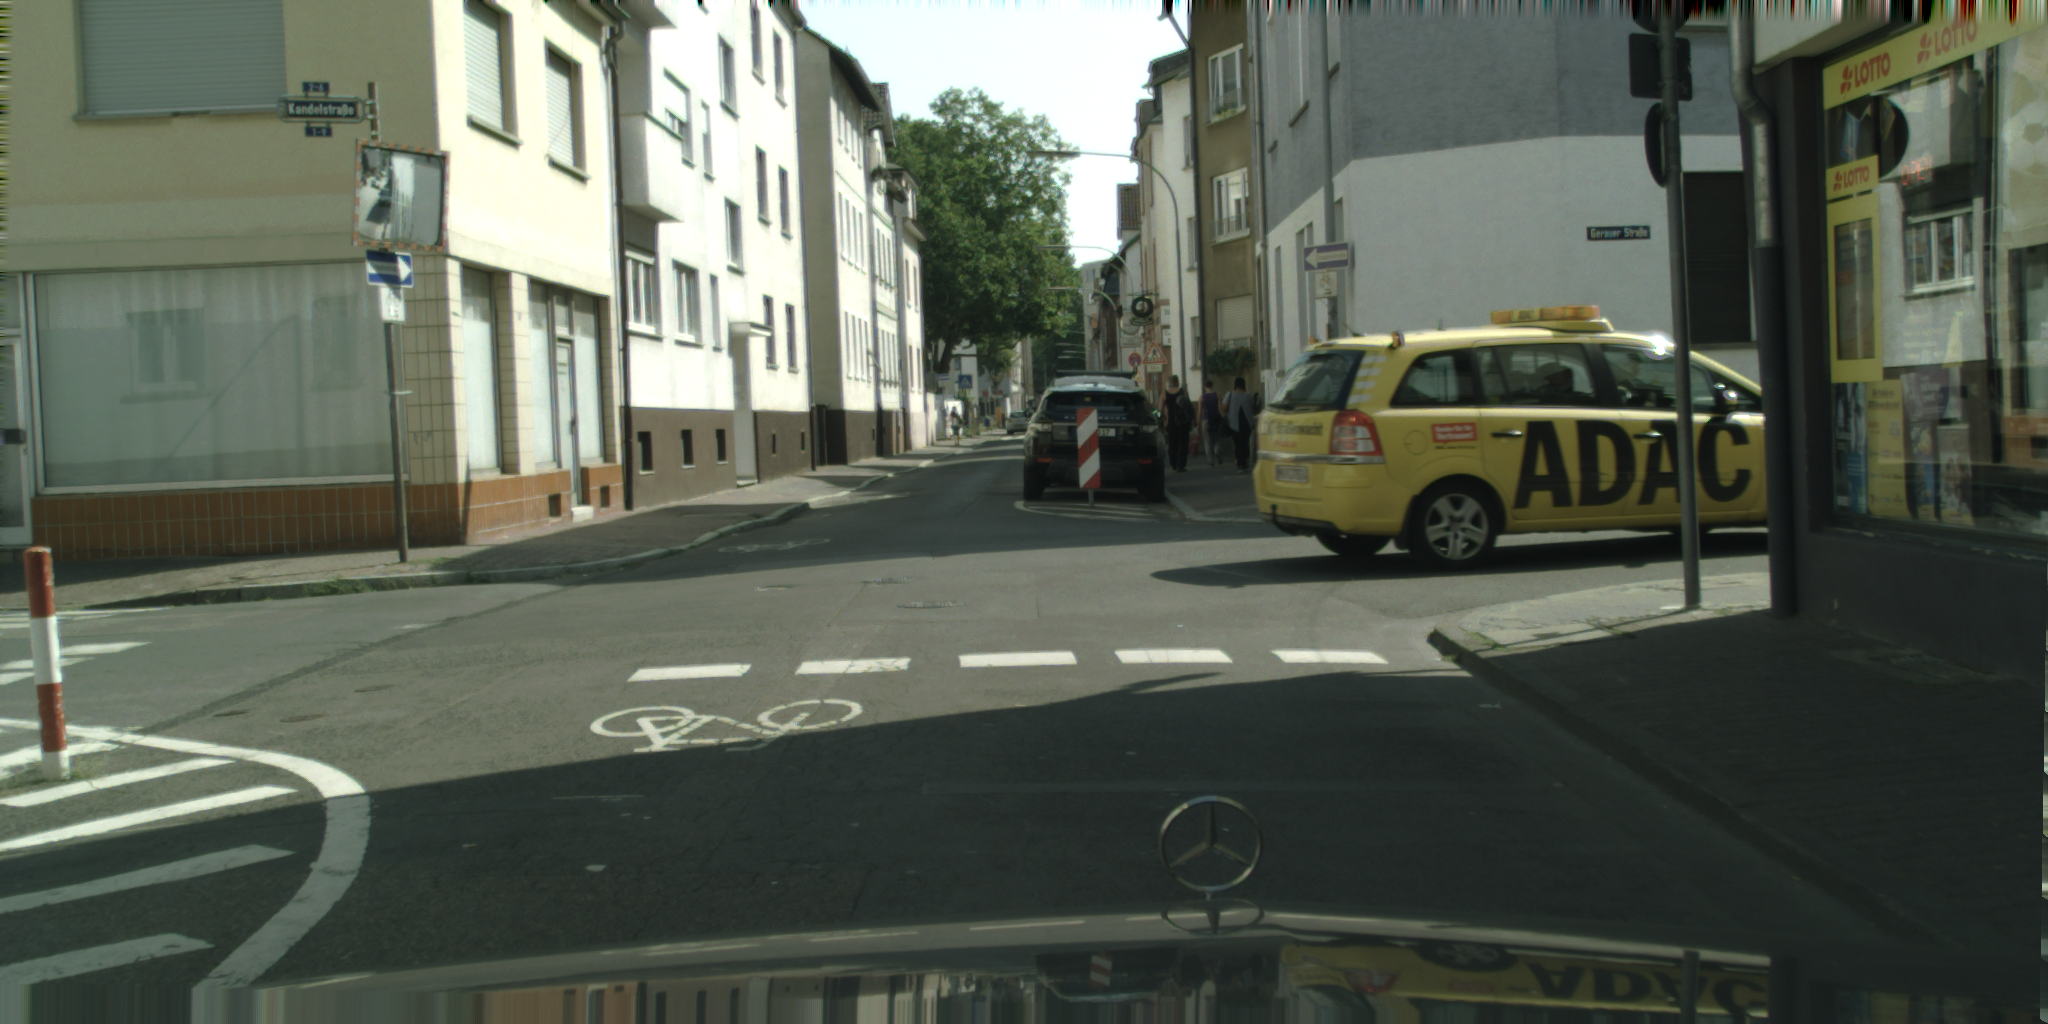
\includegraphics[width=.2\linewidth]{res/pseudo-teacher-qualitative/image.png}                     & 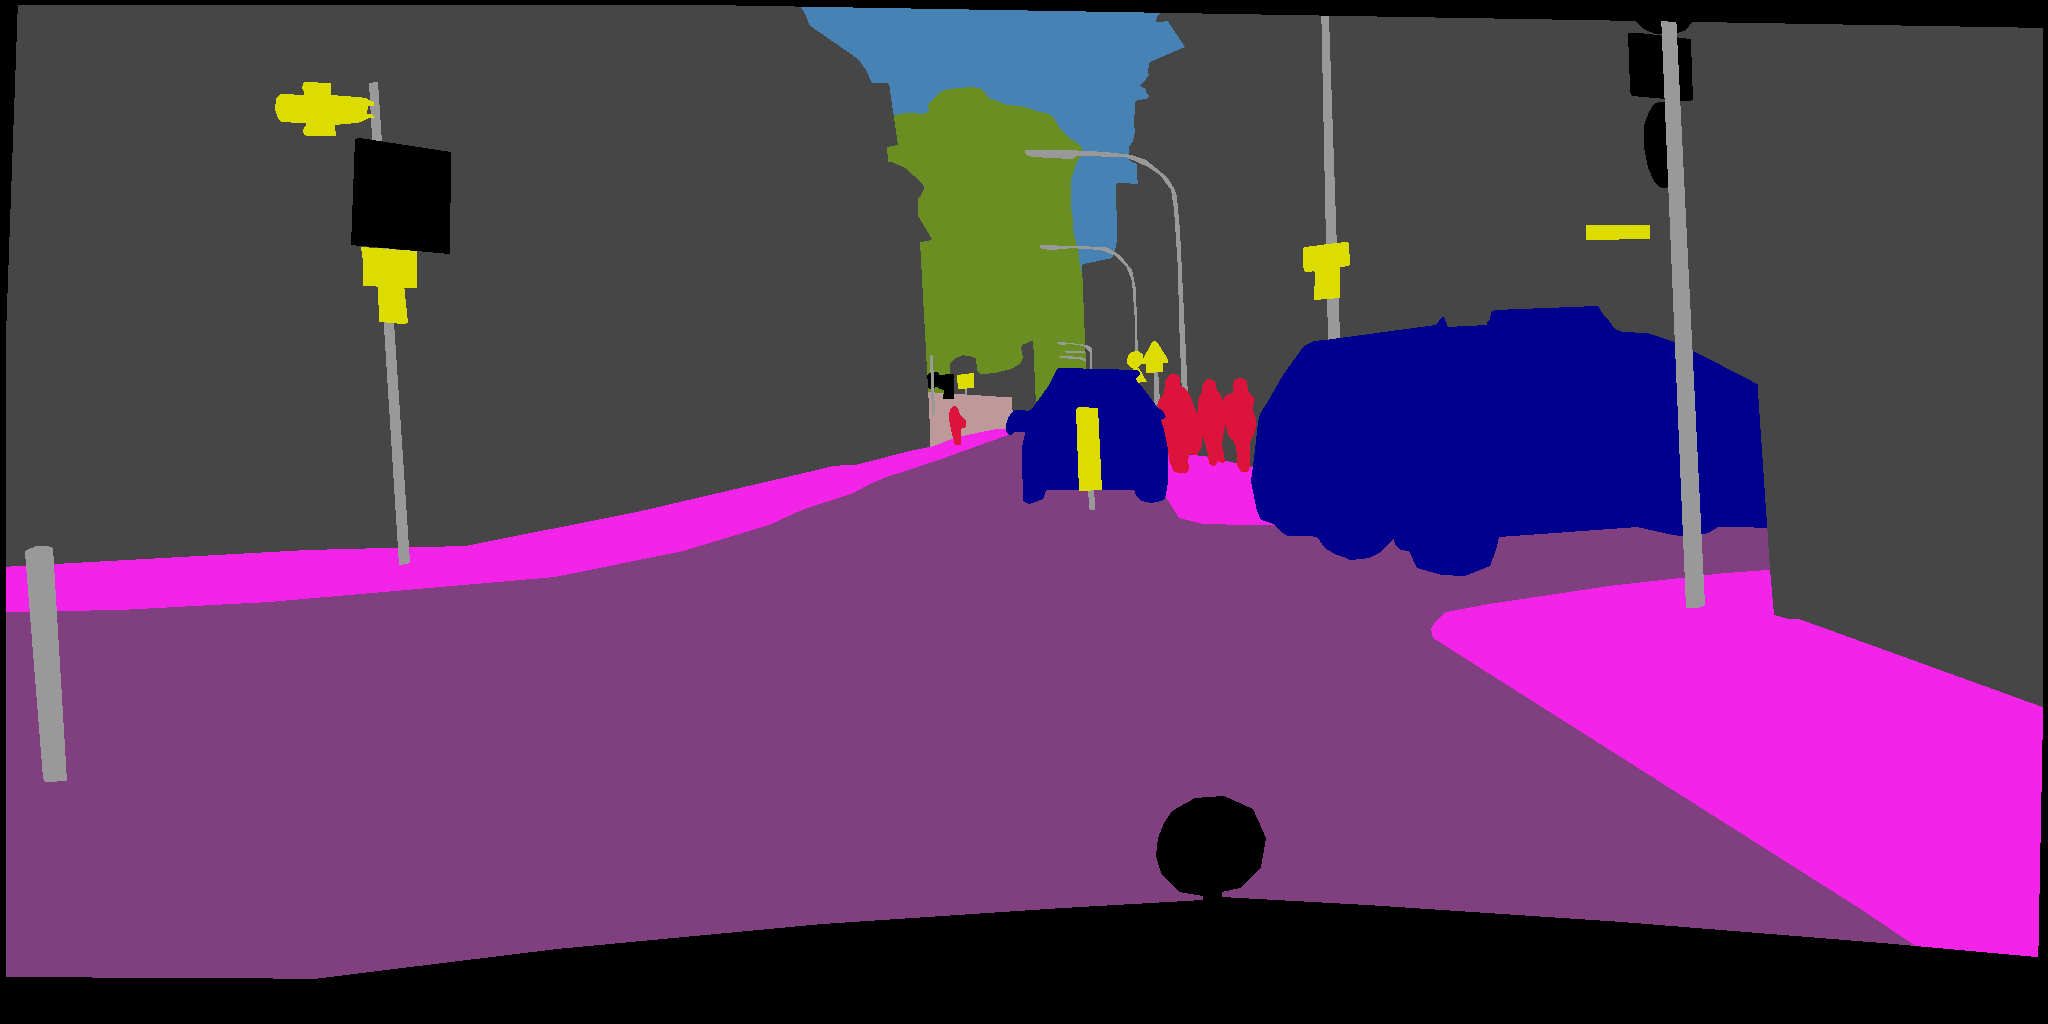
\includegraphics[width=.2\linewidth]{res/pseudo-teacher-qualitative/ground-truth.png}                  &                                                                                                         \\
                \textbf{Model} & \textbf{Approach} & \textbf{Source-Only}                                                                                        & \textbf{UDA}                                                                                                    & \textbf{Oracle}                                                                                         \\
                Topformer-Base & Pseudo-Teacher    & 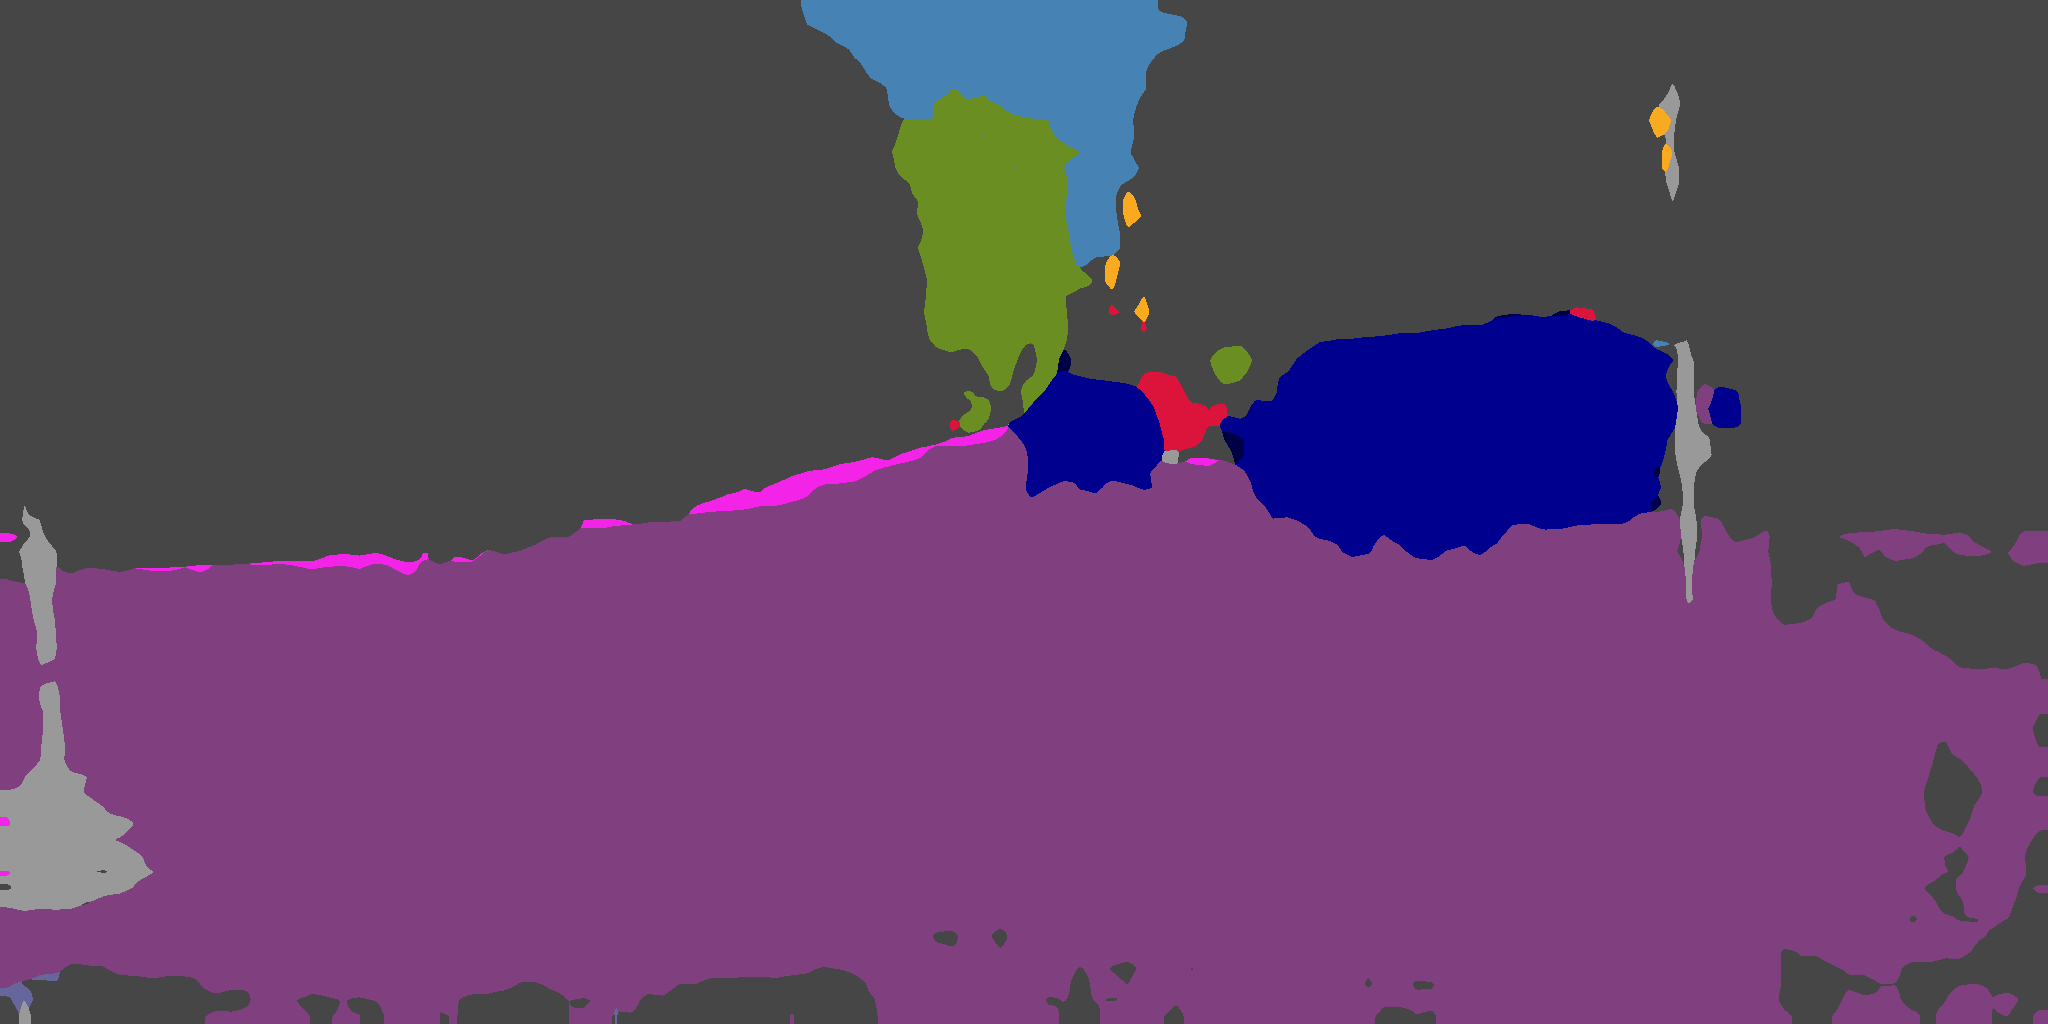
\includegraphics[width=.2\linewidth]{res/pseudo-teacher-qualitative/topformer-base-sourceonly.png} & 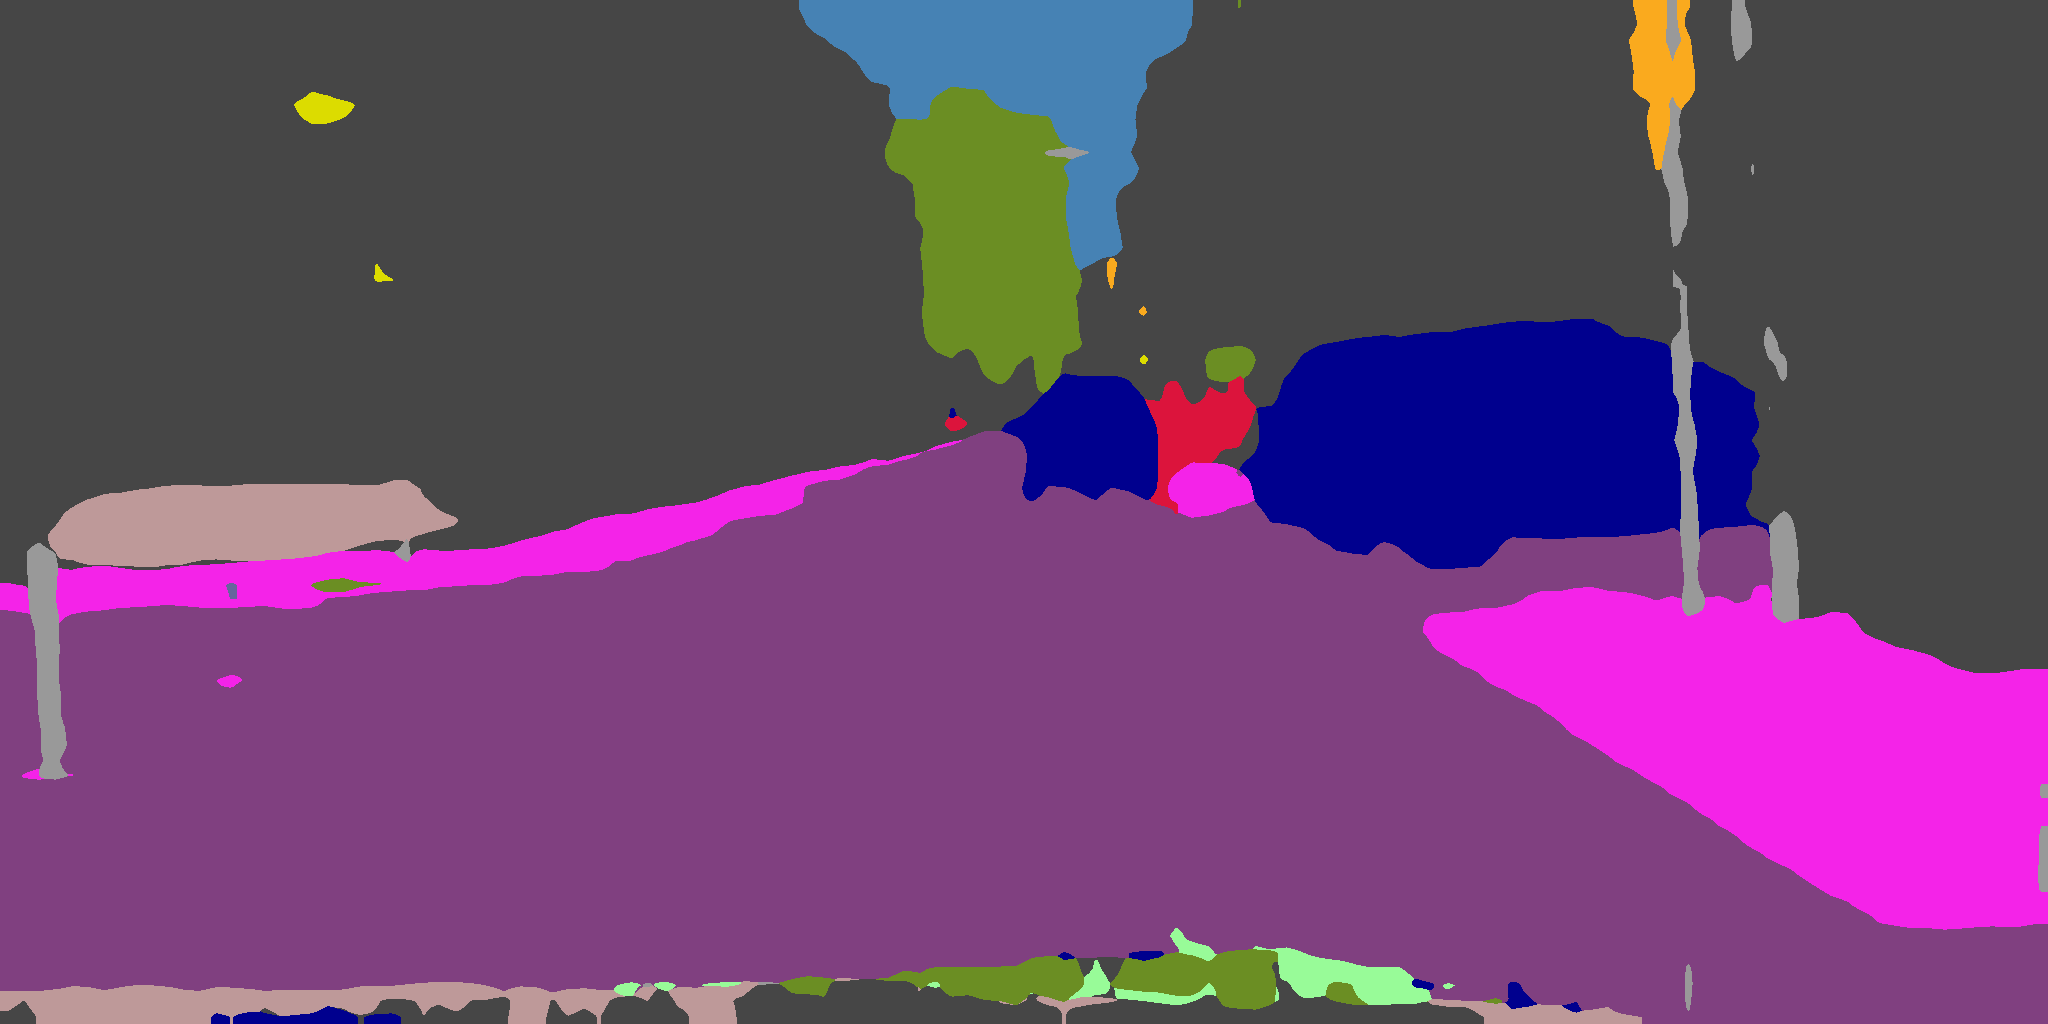
\includegraphics[width=.2\linewidth]{res/pseudo-teacher-qualitative/topformer-base-pseudo-teacher.png} & 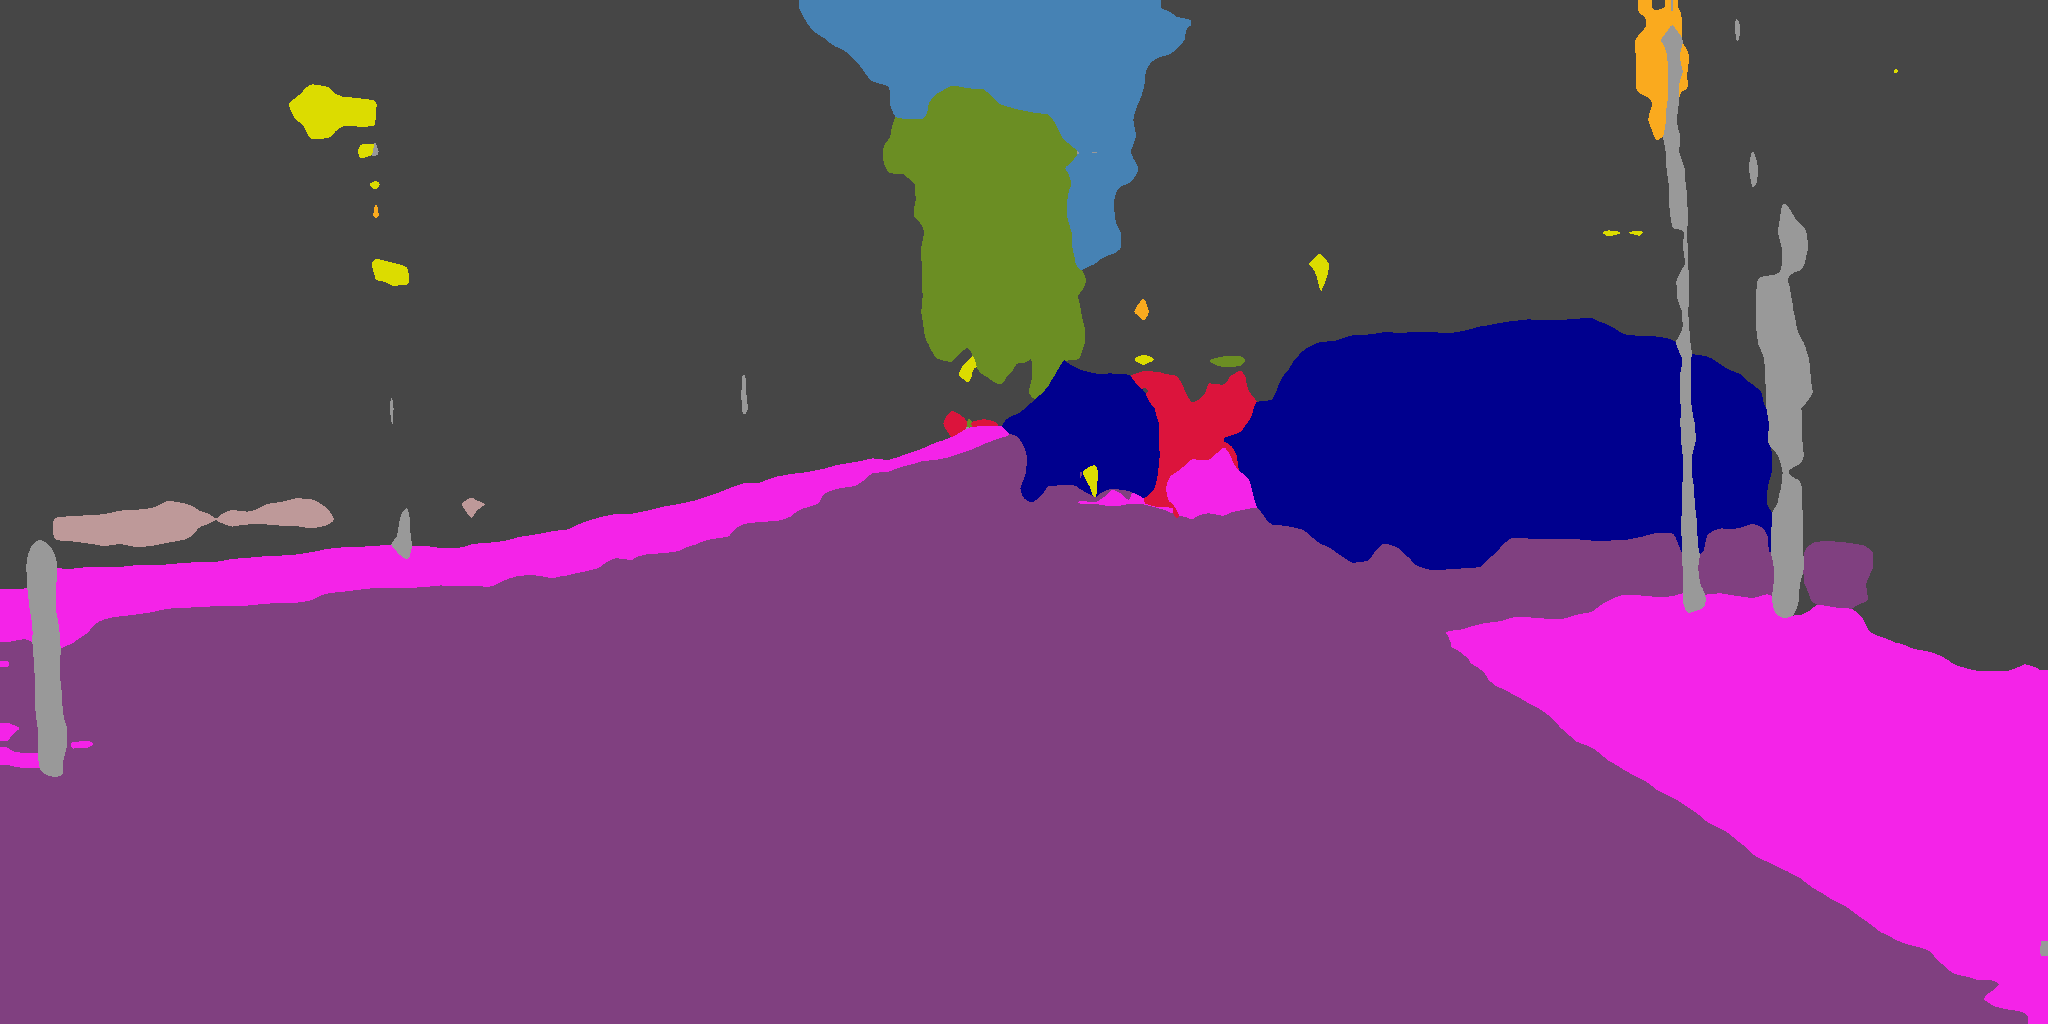
\includegraphics[width=.2\linewidth]{res/pseudo-teacher-qualitative/topformer-base-oracle.png} \\
                Topformer-Tiny & Pseudo-Teacher    & 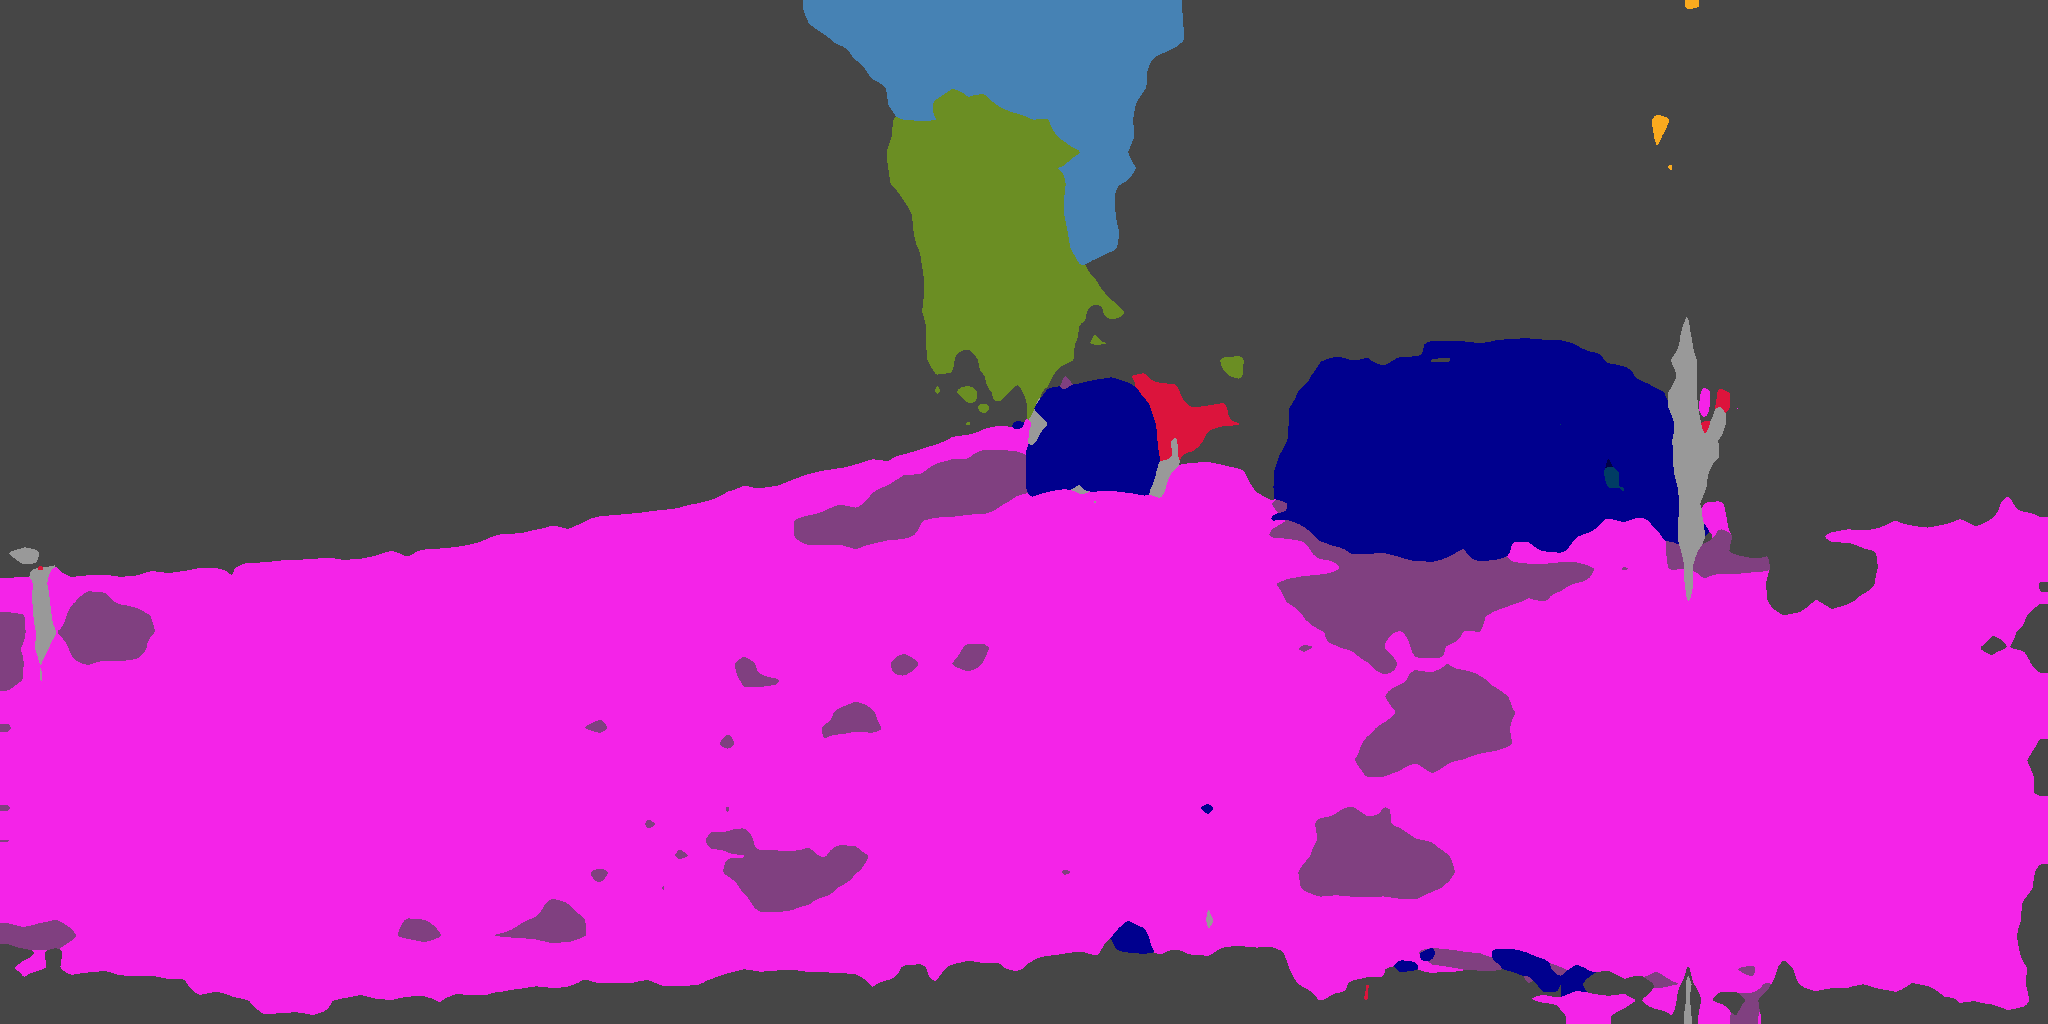
\includegraphics[width=.2\linewidth]{res/pseudo-teacher-qualitative/topformer-tiny-sourceonly.png} & 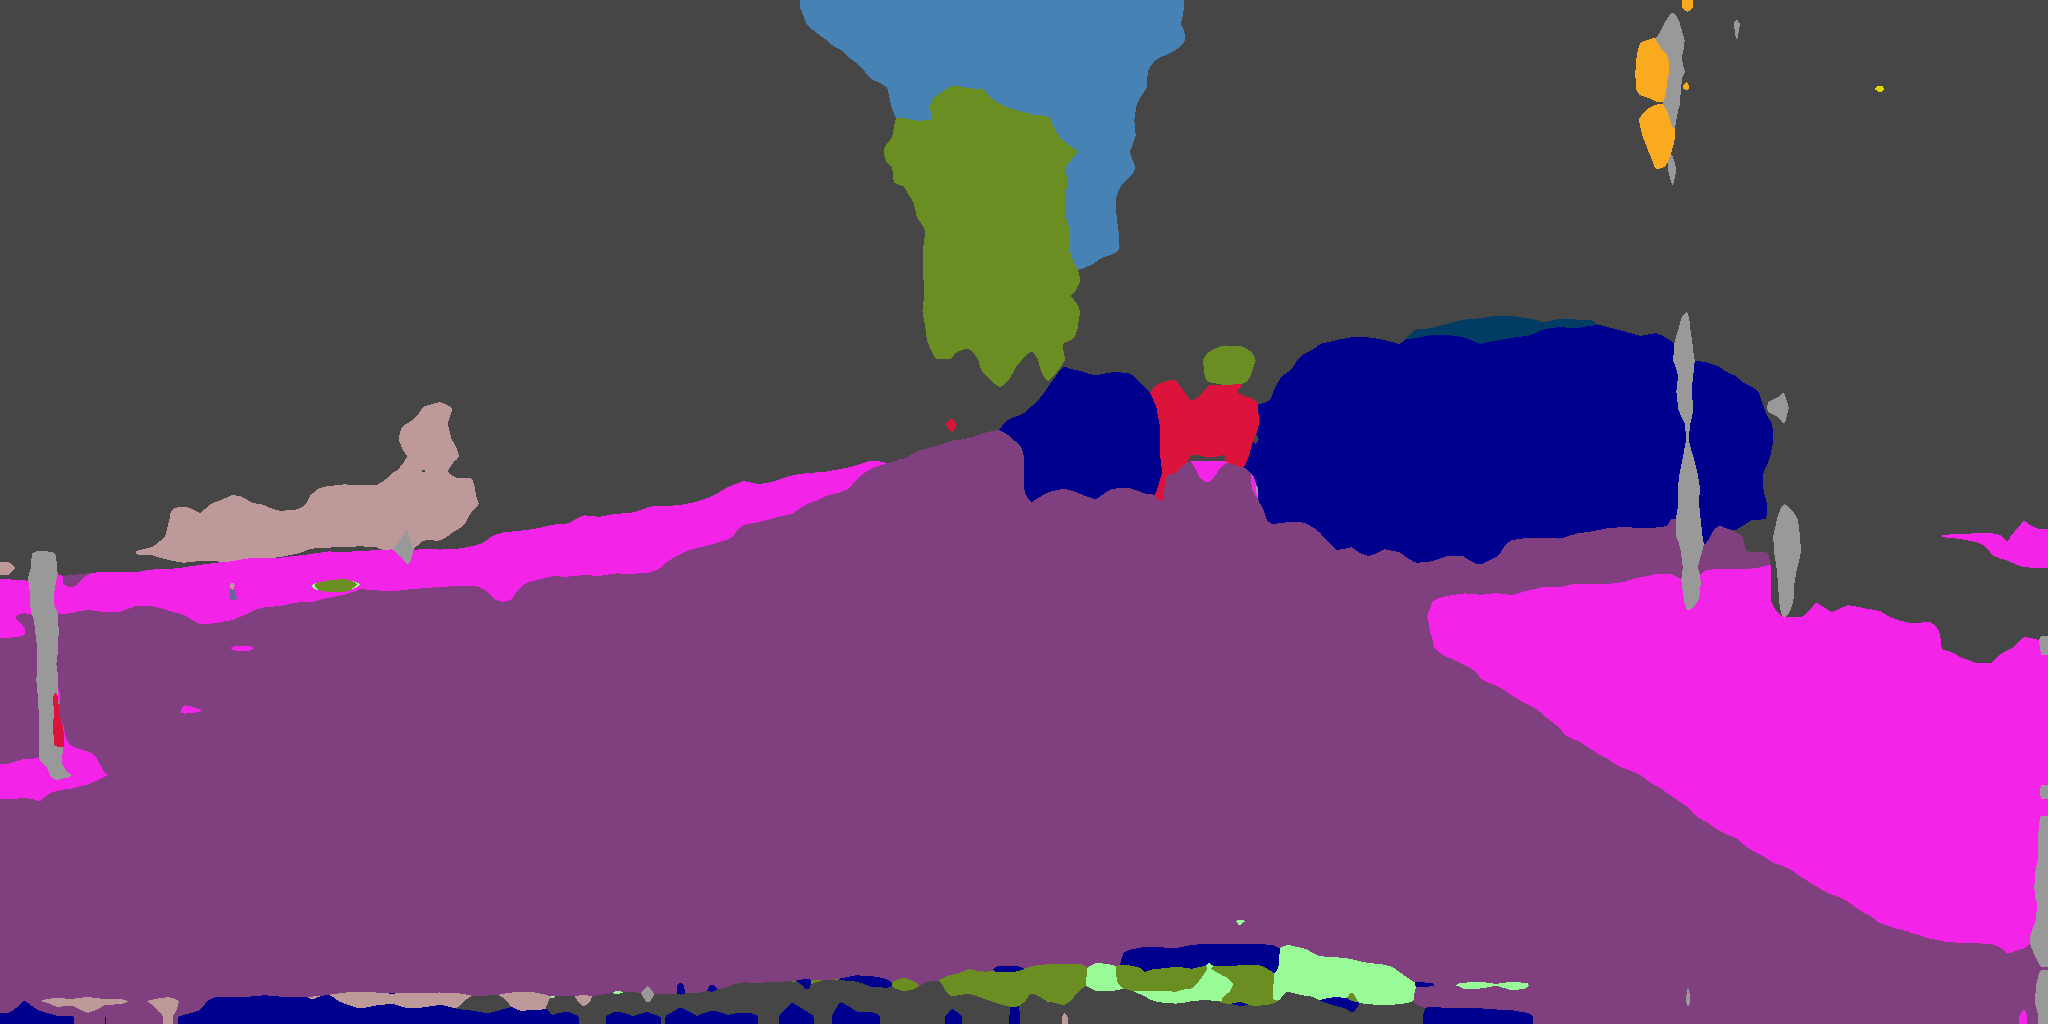
\includegraphics[width=.2\linewidth]{res/pseudo-teacher-qualitative/topformer-tiny-pseudo-teacher.png} & 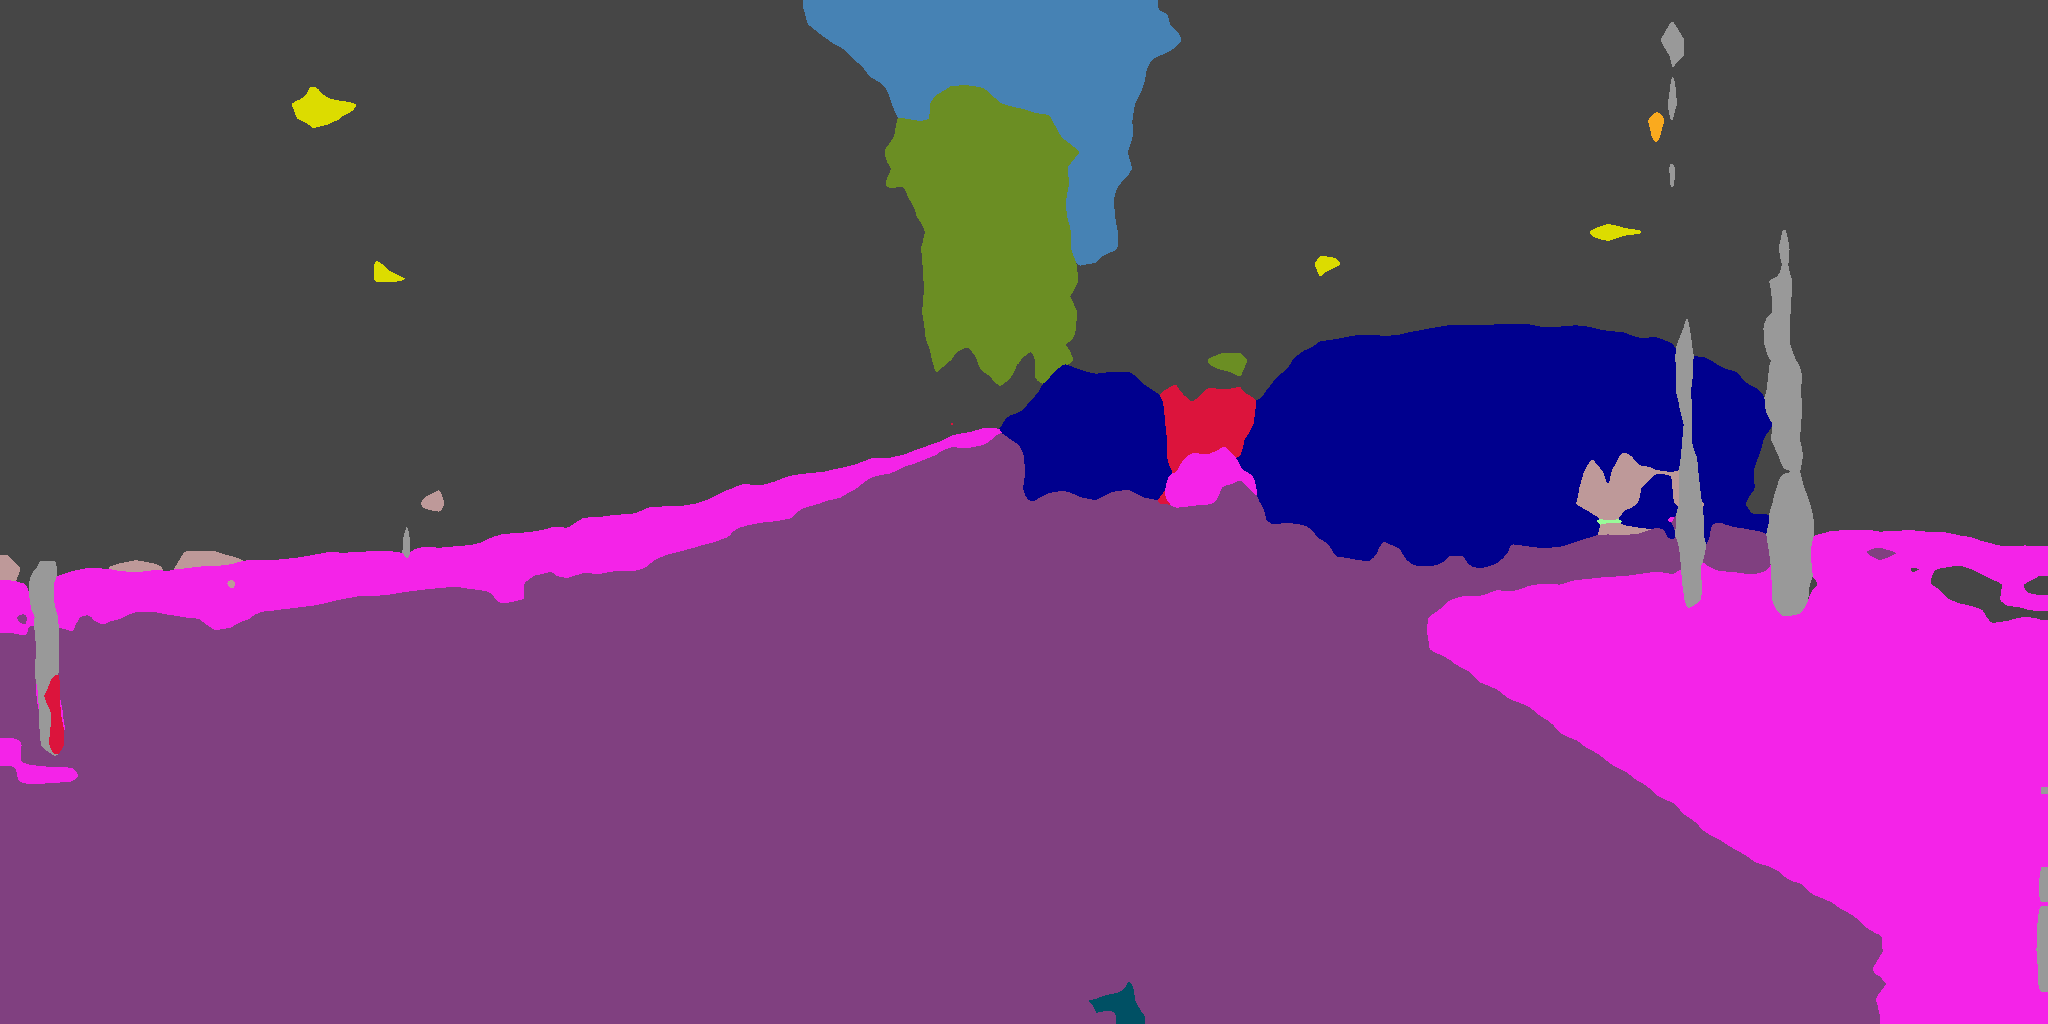
\includegraphics[width=.2\linewidth]{res/pseudo-teacher-qualitative/topformer-tiny-oracle.png} \\
                DAFormer       & Pseudo-Teacher    & 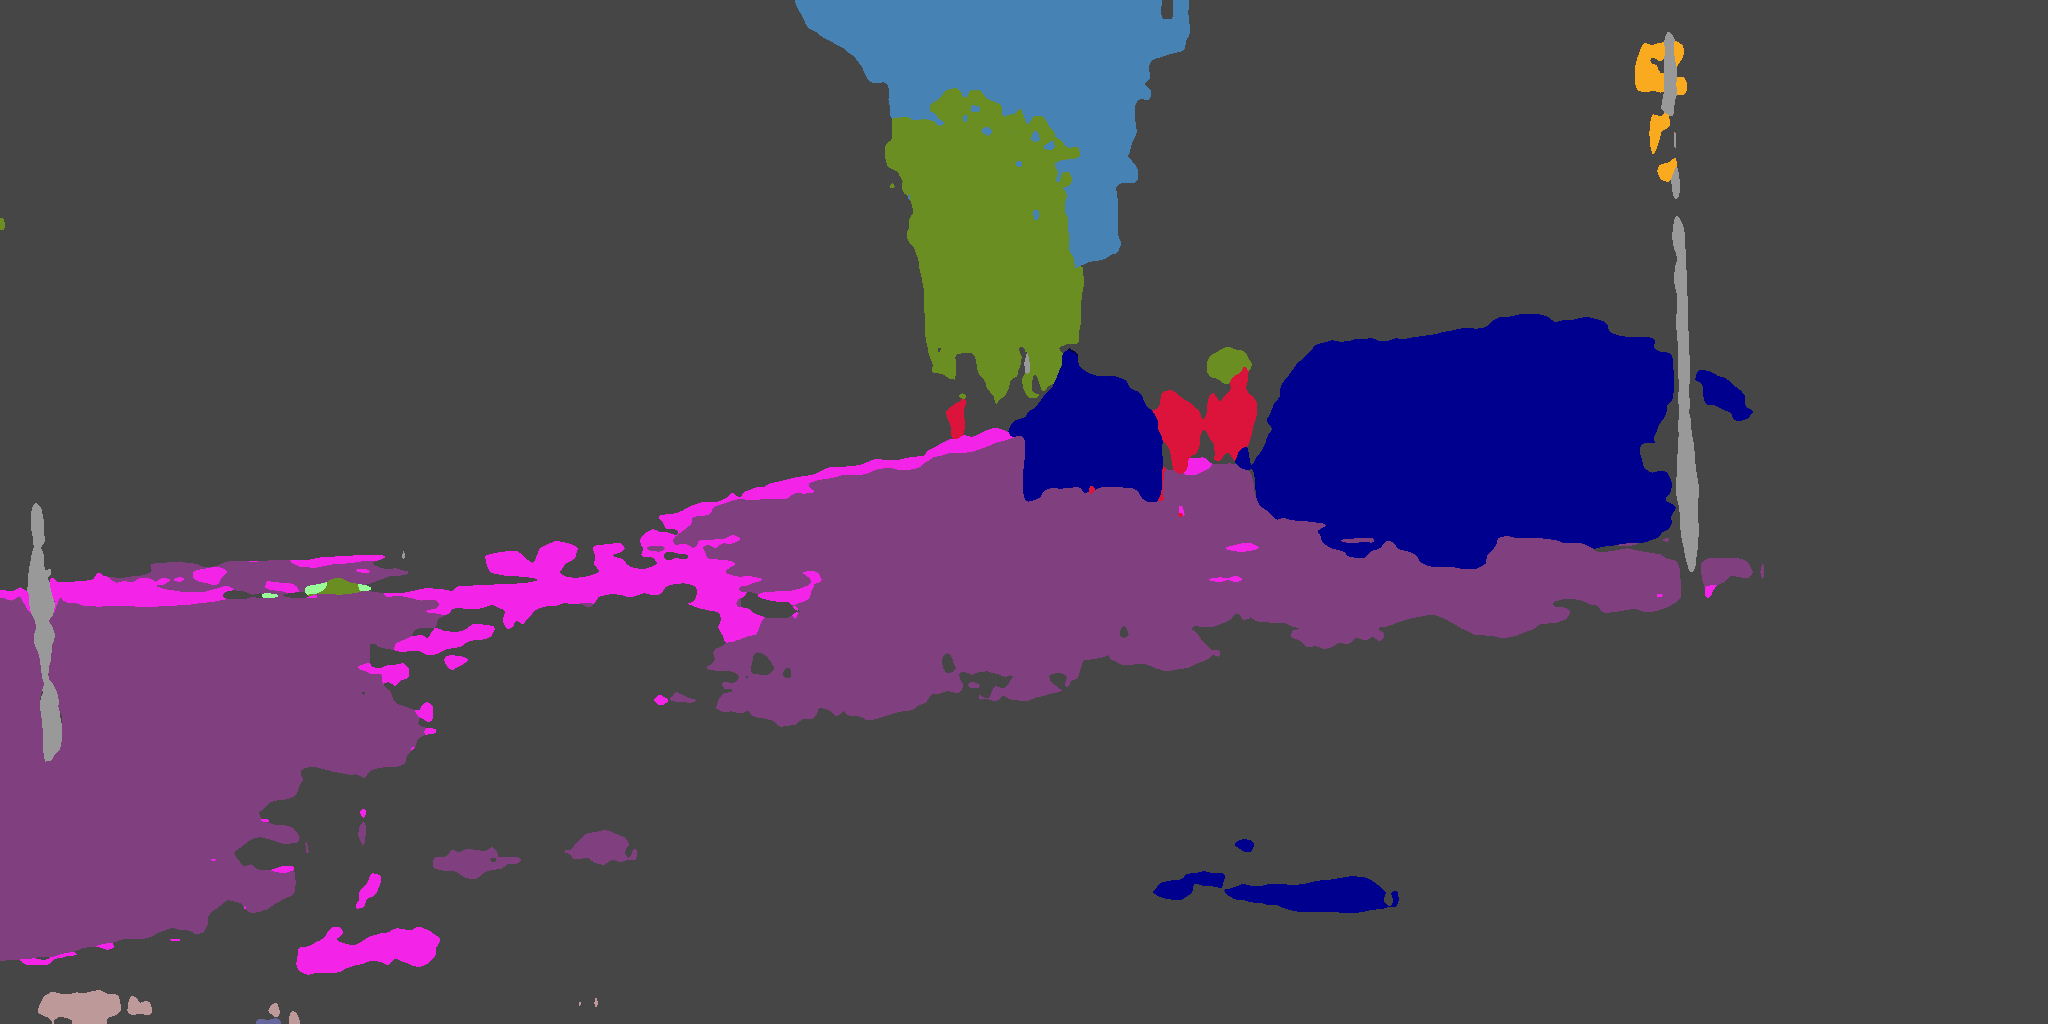
\includegraphics[width=.2\linewidth]{res/pseudo-teacher-qualitative/daformer-sourceonly.png}       & 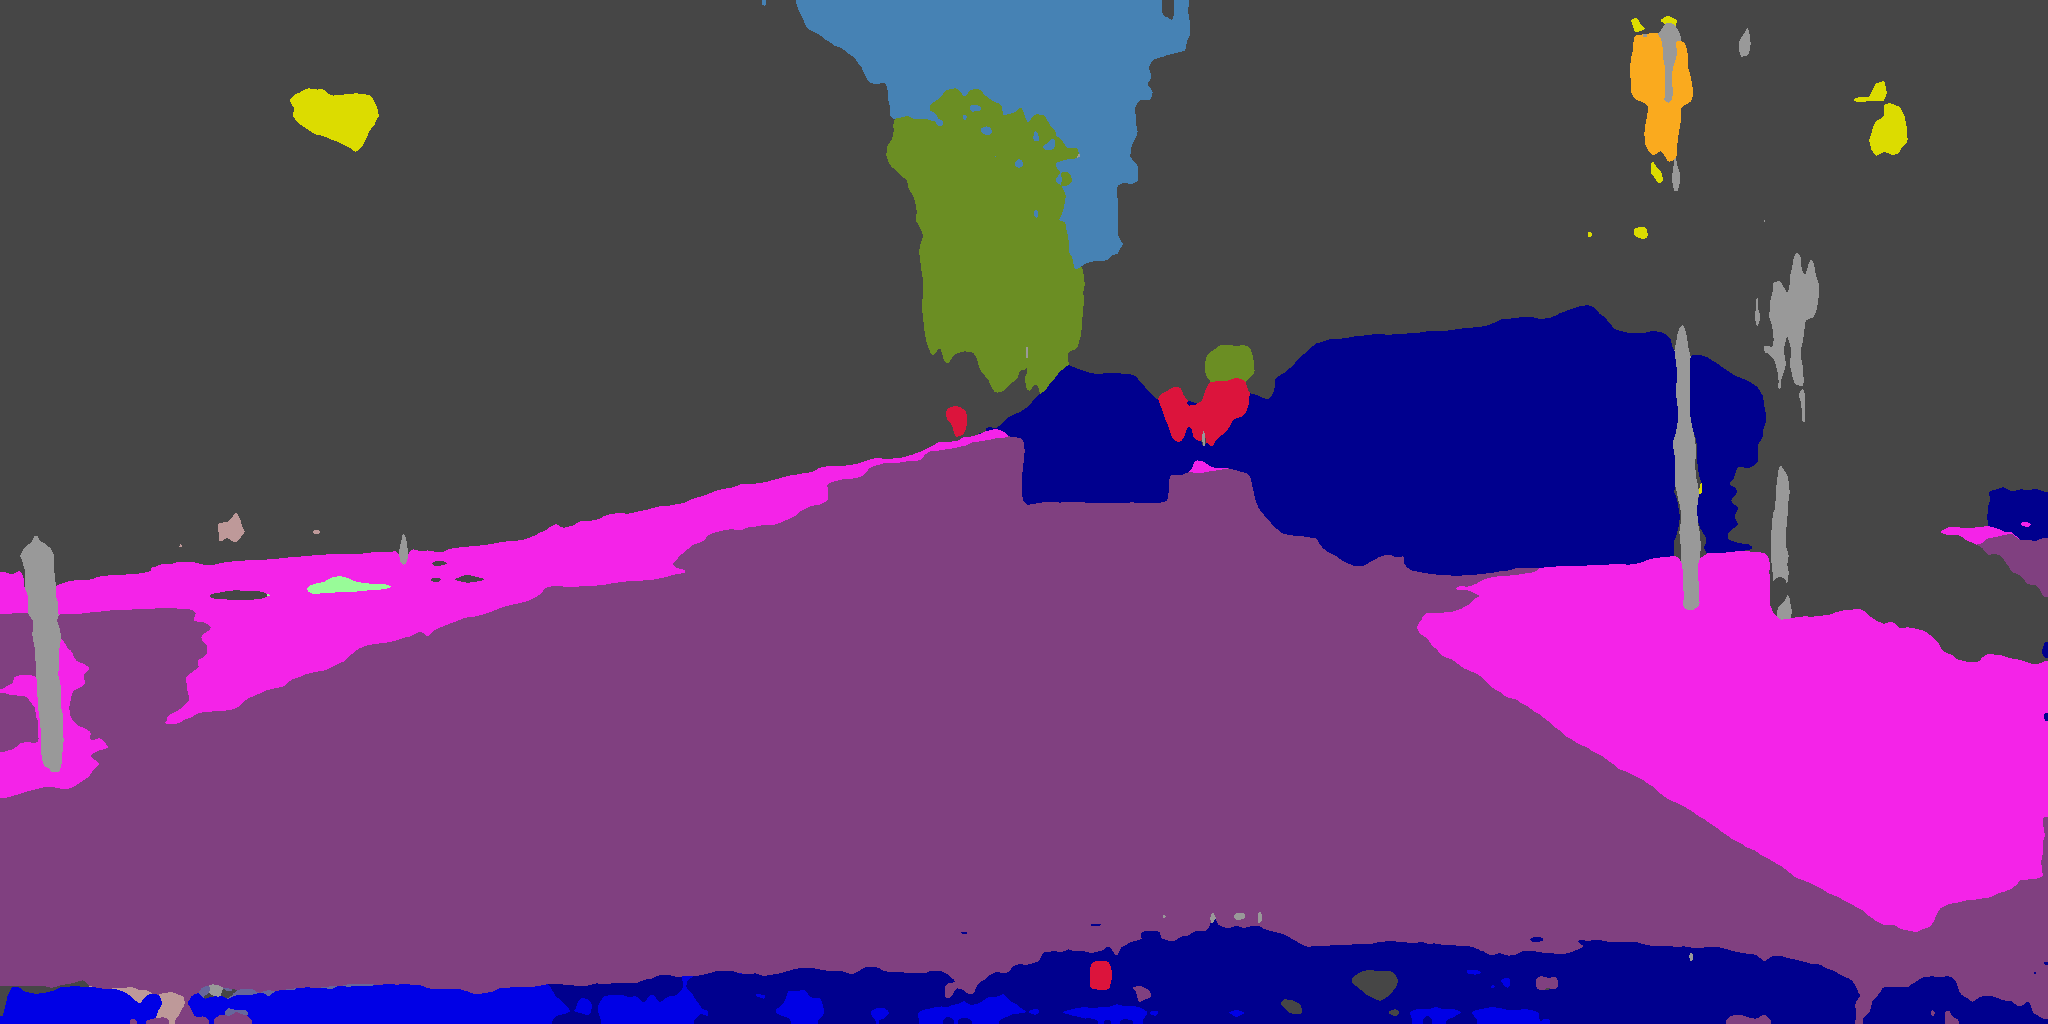
\includegraphics[width=.2\linewidth]{res/pseudo-teacher-qualitative/daformer-uda.png}                  & 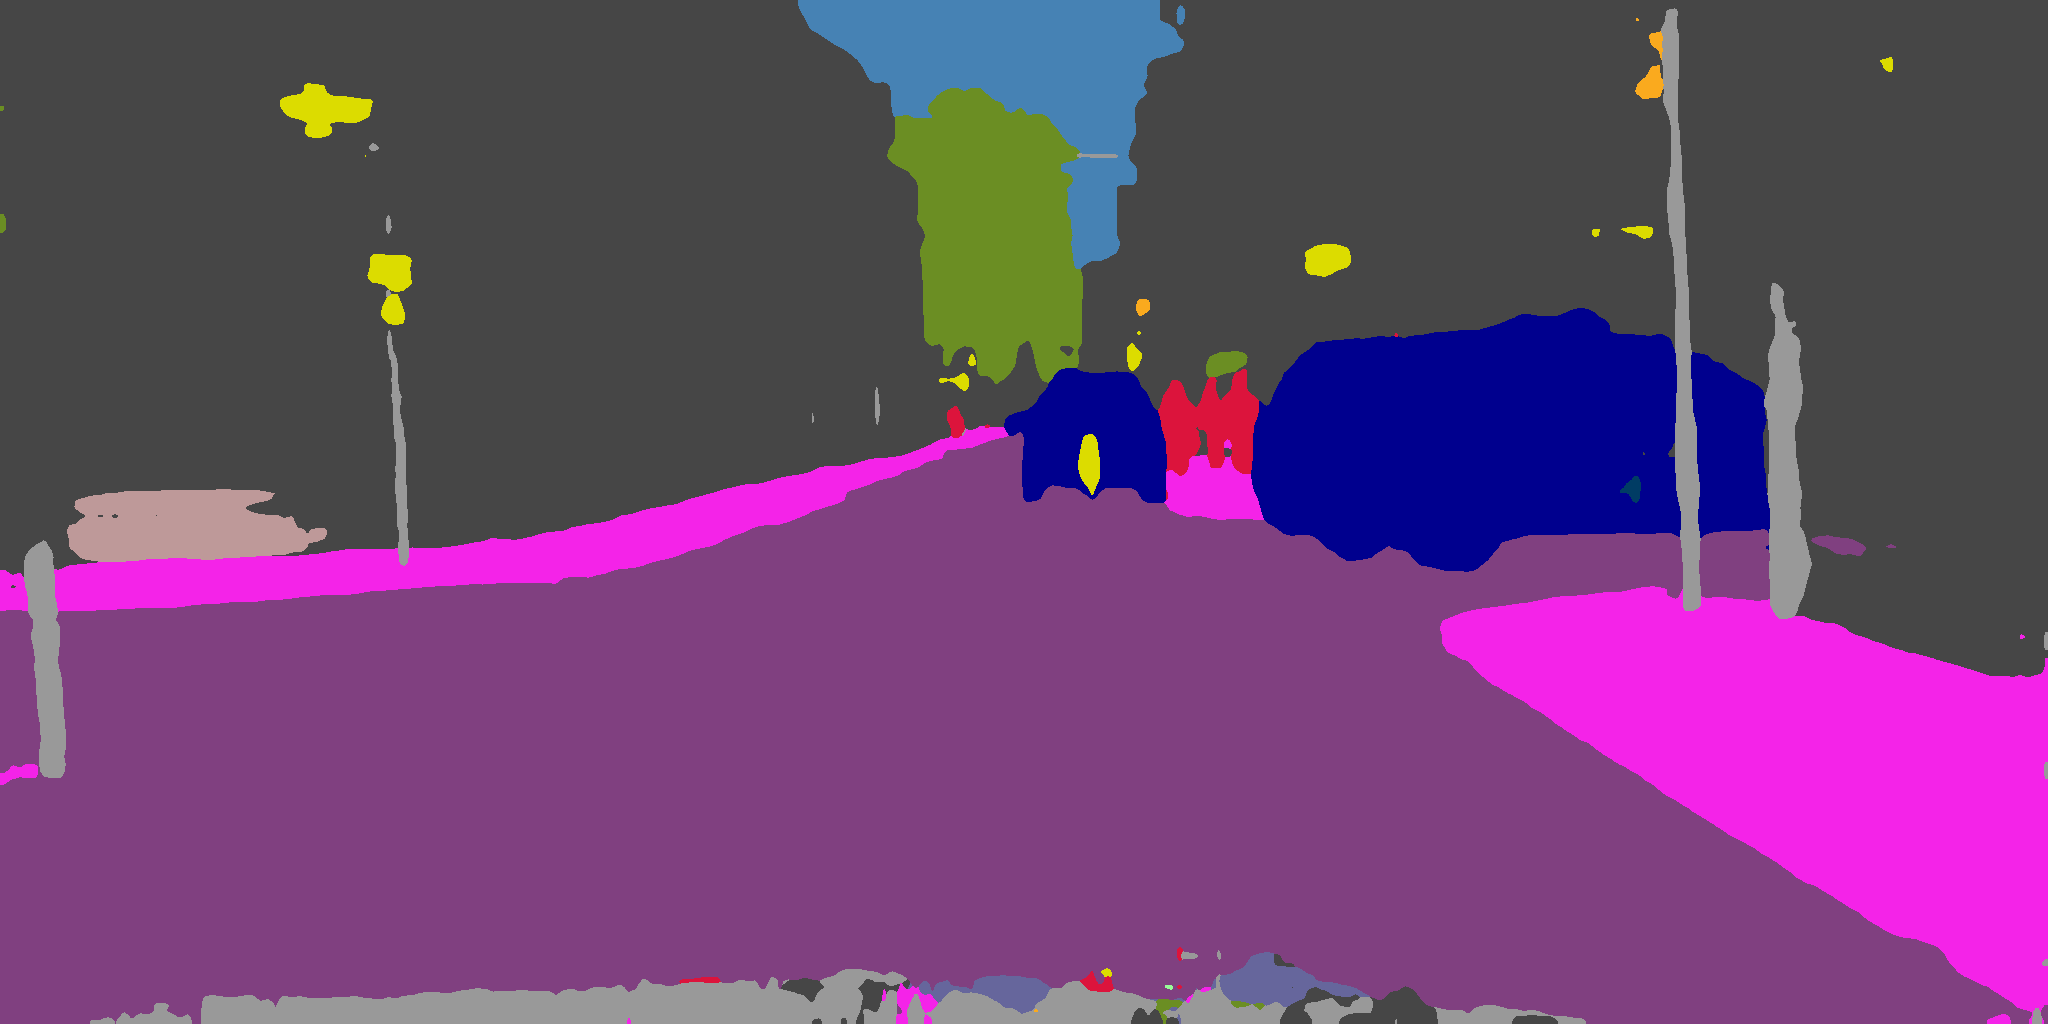
\includegraphics[width=.2\linewidth]{res/pseudo-teacher-qualitative/daformer-oracle.png}       \\
            \end{tabular}
        }
        \caption{Qualitative results of Pseudo-Teacher approach on Cityscapes dataset.}
        \label{fig:pseudo-teacher-qualitative}
    \end{table}
\end{frame}

\section{Conclusion}


% ---------------------------------------------------------------------------
%% ---------------------------------------------------------------------

%% ---------------------------------------------------------------------------
% Reference frames
% \begin{frame}[t,allowframebreaks]
%     \frametitle{References}
%     \printbibliography
% \end{frame}

%% ---------------------------------------------------------------------------
% Final frame
\begin{frame}{}
    \centering
    \huge{\textbf{\example{Thank you!}}}

    \vspace{1cm}

    \Large{\textbf{Contact:}}
    \newline
    \vspace*{0.5cm}
    \large{\email{moritz.bergemann@gmail.com}}
\end{frame}

\end{document}